\RequirePackage[table]{xcolor}
\documentclass[12pt,lot,lol,lof]{puthesis_undergraduate}
\usepackage{amsfonts}
\usepackage{amssymb}
\usepackage{amsmath}
\usepackage{amsthm}
\usepackage{latexsym}
\usepackage{graphicx}
\usepackage{setspace}
\usepackage[round, longnamesfirst]{natbib} % for nice bibliography
\usepackage{url}
\usepackage{algorithm2e}
\usepackage{listings}
\usepackage{color}
\usepackage{multirow}
\usepackage{bm}
\RestyleAlgo{boxruled}
\usepackage{courier}


\definecolor{mygreen}{rgb}{0,0.6,0}
\definecolor{mygray}{rgb}{0.5,0.5,0.5}
\definecolor{mymauve}{rgb}{0.58,0,0.82}
\lstset{ %
  backgroundcolor=\color{white},   % choose the background color
  basicstyle=\footnotesize\ttfamily,        % size of fonts used for the code
  breaklines=true,                 % automatic line breaking only at whitespace,
  postbreak=\mbox{\textcolor{red}{$\hookrightarrow$}\space},
  commentstyle=\color{mygreen},    % comment style
  escapeinside={\%*}{*)},          % if you want to add LaTeX within your code
  keywordstyle=\color{blue},       % keyword style
  stringstyle=\color{mymauve},     % string literal style
}
\newcommand{\subf}[2]{%
  {\small\begin{tabular}[t]{@{}c@{}}
  #1\\#2
  \end{tabular}}%
}

%Do not un-comment the next two lines
%Included for Gather Purpose only in WinEdt (ignore for other editors):
%input "./Bibliography/refs.bib"

\title{Using Simulated Limit Order Book Data To Evaluate Trade Execution Strategies}
\submitted{April 16, 2019}
\author{Andrew Wang}
\advisor{Professor Mykhaylo Shkolnikov}


\abstract{
The electronic nature of markets today allows traders to infer information from limit order book (LOB) data and execute trades based on this information. Agents such as hedge funds are often interested in solving what is known as the optimal trade execution problem, where they attempt to minimize cost and market impact when buying or selling a large amount of inventory. In this thesis, historical LOB data is used to simulate a market environment in which trade execution strategies can be tested. First, high-frequency LOB data from the Coinbase Pro cryptocurrency exchange is used to create a modified version of the queue-reactive model developed by Huang et al. (2013). A market simulator is built based on this model where market dynamics update in real-time in response to the agent's actions. The performance of common trade execution strategies are then evaluated in the simulated market environment. The findings from this paper are relevant for institutions who are interested in using a simulated market environment to test trading strategies before executing them.
}

\acknowledgements{
I would like to thank the many people who were instrumental to the writing of this thesis and to those who made my years at Princeton such a good time.
\newline

Thank you to Professor Mykhaylo Shkolnikov for all the help you provided throughout the year. Your expertise was essential for guiding me through the challenges I faced when writing this thesis.
\newline

Thank you to Jason and Steven for taking the time to edit my thesis. I hope you make the most of your senior year.
\newline

Thank you to Chris, Pat, Shamay, and Dora for making Dod 403 the best room on campus. Your presence made it an amazing place to live each day.
\newline

Thank you to the boys and girls of Clockwork for all the good times. Clockwork makes me so happy.
\newline

Thank you to Cap for welcoming me into your home. I'm fortunate to have been part of such an Illustrious community.
\newline

Thank you to TB for sticking with me through thick and thin. Even though we're going different places, I hope our paths cross again after graduation.
\newline

Finally, thank you to my family --- Heather, Rebecca, Tiffany, Mom, and Dad --- for supporting me my whole life. I wouldn't have made it here without you.




}

\dedication{Hammis Aequus Durando}

\begin{document}

\chapter{Introduction}\label{ch:intro}
\section{Problem Description} \label{ch:problemdescription}

This thesis analyzes a problem in quantitative finance known as the optimal trade execution problem. In essence, when trading a large volume of a security in a short amount of time, I seek to minimize “slippage”, which is the difference between the expected price of a security and the price at which the trade is actually executed. More formally, given a volume $V$ of a security to buy and a time limit $T$, I seek to limit the amount of money spent to acquire these shares. Similarly, we could be given an amount $V$ to sell and a time limit $T$, and seek to maximize the revenue received from selling the security. 

This problem is most relevant to a large institutional investor, such as a hedge fund, who may want to buy (respectively, sell) a large volume of a security because they believe that the price of the security will rise (fall), but find that there is not enough supply (demand) at the desired price level to satisfy the full order. If the full trade could be executed at the desired price, the hedge fund would want to execute the trade immediately in order to capture as much of the expected change in price as possible. However, the hedge fund would have to execute part of the trade at more unfavorable prices. They can instead choose to split the order over a longer time period to minimize slippage. In general, there is a trade-off between how quickly the desired position is achieved and the price impact of the trade.


\section{Background} \label{ch:background}
This problem can be illustrated more clearly by discussing the centralized limit order book (LOB). The LOB is the trading mechanism used by most exchanges around the world. The LOB for a security consists of the prices and volumes at which customers are willing to buy and sell the security (bids and asks respectively). For example, part of the LOB for Coca-Cola (KO) on the NYSE may look like Table~\ref{tab:coke1}, in which the 5 best bids and asks are listed:

\begin{table}[htbp]
\caption{Coca-Cola Limit Order Book} \label{tab:coke1}
\begin{center}
\begin{tabular}{ll|ll}
\hline \hline
\multicolumn{2}{l|}{\textbf{Bids}} & \multicolumn{2}{l}{\textbf{Asks}} \\
\hline
Volume           & Price          & Price           & Volume          \\
\hline
1000             & 48.69          & 48.70           & 500             \\
2000             & 48.68          & 48.71           & 1500            \\
3000             & 48.67          & 48.72           & 3500            \\
6000             & 48.63          & 48.75           & 2400            \\
8000             & 48.58          & 48.80           & 10000          
\end{tabular}
\end{center}
\end{table}

The price of the stock could be considered \$48.695, which is the midpoint between the best bid and best ask price. 

Say, for example, that the hedge fund receives a signal to buy 7000 shares of Coca-Cola. It could do so by issuing a market order, in which the trade is executed immediately at the best market price(s). If there is not enough supply at the best ask price, the order will progressively move up the order book until it is satisfied. In this case, it would buy 500 shares at \$48.70, 1500 shares at \$48.71, 3500 shares at \$48.72, and the remaining 1500 shares at \$48.75. It could also place a limit order, which is only executed at the specified price or better. For example, it could place a limit order for 7000 shares at \$48.67. This order would be appear in the bid side of the order book until it is matched with a market order from the ask side. The updated LOB is shown in Table~\ref{tab:coke2}.

\begin{table}[htbp]
\caption{Coca-Cola Updated Limit Order Book} \label{tab:coke2}
\begin{center}
\begin{tabular}{ll|ll}
\hline \hline
\multicolumn{2}{l|}{\textbf{Bids}} & \multicolumn{2}{l}{\textbf{Asks}} \\
\hline
Volume           & Price          & Price           & Volume          \\
\hline
1000             & 48.69          & 48.70           & 500             \\
2000             & 48.68          & 48.71           & 1500            \\
\underline{10000}             & \underline{48.67}          & 48.72           & 3500            \\
6000             & 48.63          & 48.75           & 2400            \\
8000             & 48.58          & 48.80           & 10000          
\end{tabular}
\end{center}
\end{table}

Exchanges typically institute a time priority policy, which means that orders submitted at the same price are executed in the order at which they arrived. Although the limit order has a maximum price at execution, it is not guaranteed to execute unlike the market order. 

Of course, it could also place multiple market or limit orders over time to achieve the desired position while minimizing market impact. Given a time horizon T and the state of the order book at each time step, we seek to find the optimal placement of market and limit orders to achieve the desired position. I will use the common industry benchmark of Volume Weighted Average Price (VWAP) to measure performance of our trading strategy:

$$ \frac{\sum{\text{Volume} * \text{Price}}}{\sum{\text{Volume}}}$$

In the case of market order example, the VWAP would be (500*48.70 + 1500*48.71 + 3500*48.72 + 1500*48.75)/7000 = \$48.723/share.



\chapter{Literature Review}\label{ch:litreview}
\section{Past Approaches to Analyzing Optimal Trade Execution}
Various approaches have been taken in the past to tackle the optimal trading execution problem. Several studies solve the optimal trade execution problem under different mathematical models of the asset price movement. \cite{A1} formulate a theoretical solution for optimal trade execution that is based on trading off execution cost mean and variance. They develop a closed form solution that maximizes expected utility of the trade at a given level of risk aversion. \cite{A1a} and \cite{A1b} expand upon this work by solving optimal trade execution under the assumption that the asset price follows a geometric Brownian motion. 

Studies have also been conducted using historical LOB data. Several studies use machine learning techniques on high-frequency data from exchanges to develop optimal trade execution methods. \cite{A5} use genetic algorithms to develop an optimal trading strategy using Australian Stock Exchange data. \cite{A4} apply reinforcement learning to optimize market making actions using equities data from across various stock market exchanges. \cite{A3} use reinforcement learning to solve the problem for several stocks listed on the NASDAQ. The studies back-test the strategies on historical data, but assume that the agent's actions do not affect the future dynamics of the LOB.

This thesis seeks to evaluate trading strategies in a realistic market environment with the impact of the agent’s actions taken into account. In order to accomplish this, an LOB must be simulated that reflects realistic market behavior. \cite{A10a} and \cite{A10b} perform statistical analysis on the empirical studies of LOBs across major exchanges. It is difficult to reflect all the properties of empirical LOBs, but studies have modelled important aspects of LOB dynamics. \cite{A11} use a supply and demand framework of LOB behavior to formulate optimal trade execution strategies involving both discrete and continuous trades. \cite{A2} expand upon this work, allowing for general LOB shapes specified density functions.

\section{LOB Queuing Model} \label{modelLOB}
Queuing models have shown promise in providing a simple model for LOB dynamics that reflect empirical properties. \cite{A6a} provides a model of the LOB where orders follow a Poisson arrival process. allowing for statistical predictions on market behaviors. \cite{A6b} model the LOB as a Markovian queuing system and estimate parameters based on data from the Tokyo stock exchange. They then use Laplace transform methods to estimate the conditional probabilities of market events based on the shape of the LOB, finding that the model provides insights on LOB behavior in the short-term. Studies have also used models similar to the queuing model where arrivals follow Poisson processes. For example, \cite{A9} modelled price jumps of an asset using a bi-dimensional Hawkes process. This model reflects several desirable properties of modern electronic markets such as its endogenous nature, where orders are correlated and made in response to each other. \cite{A6} develop a model where the LOB is a multi-dimensional queuing system centered around the mid-price of the asset. This model lends itself to easily estimating parameters from market data and accurately reproducing market behavior. This thesis uses a modified version of the model, which is described below:

The LOB is modelled as a $2K$-dimensional vector $Q$, where $K$ is number of prices on each side of the Markovian queuing system. Let $p_{ref}$ be the reference price of the of the stock. Then, $[Q_k: k = -1 \ldots -K]$ represents the number of orders on the bid side $k - 0.5$ ticks to the left of $p_{ref}$ and $[Q_k: k =1 \ldots K]$ represents the number of orders on the ask side $k - 0.5$ ticks to the right of $p_{ref}$. Then, $$Q(t) = (q_{-K}(t), … q_{-1}(t), q_1(t), … , q_K(t))$$ is a continuous-time Markov jump process with a jump size equal to one.

An event at position $k$ occurs any time that the number of shares offered at position $k$ changes. It increases when a trader places a limit order at the price of position $k$ and decreases when it is either consumed by a market order from the other side or the trader cancels the limit order.

The simplest model assumes that $Q_k$ is independent for each $k$. Each jump when $Q_k$ increases by 1 and $Q = q$ follows a Poisson arrival with rate $\lambda^+_k(q)$ and each jump when $Q_k$ decreases by 1 and $Q = q$ follows a Poisson arrival with rate $\lambda^-_k(q)$. In order to model each $Q_k$ as a positive integer with changes equal to 1, we use $Q_k$ to represent the number of Average Event Sizes ($AES_k$) present at the LOB position. $AES$ is the average size of the absolute change in the number of shares at the queue position whenever a change occurs, where each $AES_k$ could differ. In this model, $Q_k = n$ would mean that there are $n*AES_k$ shares offered at position $k$.

We choose $p_{ref}$ to be a price in between 2 adjacent ticks, so that events at each position occur at actual tick prices. Let $p_{-1}$ be the best bid price and $p_1$ be the best ask price. If $p_{-1}$ and $p_1$ are an odd number of ticks apart, then we have 
$$p_{ref}=  (p_{-1}+p_1)/2$$
If $b$ and $a$ are an even number of ticks apart, then we could pick $p_{ref}$ to be $(p_{-1}+p_1)/2 + 0.5$ or $(p_{-1}+p_1)/2 - 0.5$. We choose the one that is closest to the previous reference price.

If an event occurs that changes the best bid or ask, then we update $p_{ref}$. It can be seen that under certain conditions, this LOB model follows an ergodic Markov process. We can then use historical LOB data to estimate $AES_k$, $\lambda^+_k(q)$, and $\lambda^-_k(q)$ for each $k$.

In simulating the LOB, this thesis examines the assumptions made in this model using market exchange data. Modifications of the model are made to more accurately reflect observations from the data set, as described in Section \ref{ch:queue_model}. A market simulator is then built based on this queuing model where trade execution strategies are tested.

\chapter{Data Source}\label{ch:data_source}
\section{Coinbase Exchange}

To simulate a real world security, high frequency LOB data of cryptocurrency securities is collected from Coinbase Pro. Coinbase Pro (formerly known as Global Digital Asset Exchange or GDAX) is the advanced trading platform of the Coinbase, which is an exchange founded in 2012 that brokers trades of many cryptocurrencies as well as fiat-currency to cryptocurrency exchanges. Major cryptocurrencies that are traded on Coinbase Pro include Bitcoin, Bitcoin Cash, Ethereum, Ethereum Classic, and Litecoin, while fiat-currencies are typically the USD or Euro. As of December 2018, Coinbase Pro has a total daily trading volume of about \$70 million (\cite{L1}). Coinbase Pro was chosen as the data source since it has readily accessible real-time LOB data that is freely available to developers from its API. It also features relatively liquid securities with large trading volumes. 

Although the LOB dynamics of the securities modelled in this paper may not entirely reflect those of securities from other exchanges such as stocks, futures, etc., the methodology in this paper is adaptable to the LOB data of any type of any relatively liquid security. The trading rules of Coinbase Pro are representative of most exchanges around the world. Coinbase Pro allows limit and market orders with time priority matching. It also allows stop orders, which is an order to place a limit or market order when the price of the security reaches a specified price. Coinbase Pro also differentiates between “maker” and “taker” orders. Taker orders are orders that fill immediately (such as market orders) and maker orders are orders that do not fill immediately and thus populate the LOB (such as limit orders). The fee structure, which is up to 0.3\% for taker orders depending on the volume and 0\% for maker orders encourages market making and therefore increases liquidity of the market. There are also rules to prevent self-trade, which is when the same trader acts as both the maker and taker for a trade. In addition, there are minimum and maximum orders for each security. Full trading rules for Coinbase Pro can be found on its website (\cite{L2}).

\section{Data Collection}
Data is collected through the Coinbase Pro API using a Python library called CoPrA, which is an asynchronous web socket client (\cite{L3}). Specifically, the ``level2" channel, which provides first provides a snapshot of the LOB. It also provides updates at every position of the LOB whenever an order happens. See listing \ref{data-collection-code} for the code written for data collection. Using these updates, an internal LOB is maintained for using during data analysis. Data was collected for several days in the months of December and January of all the updates on the ETC-USD LOB (Ethereum Classic for USD), which has around \$2 million volume of trades each day (\cite{L1}). The initial LOB is shown in Figure \ref{fig:12_30_18_LOB_pic}. The 10 best bids and asks are shown, which is where the vast majority of updates are made, but updates are also recorded for prices farther from the reference price.

\begin{figure}[t]
\begin{center}
\caption{LOB Sample}
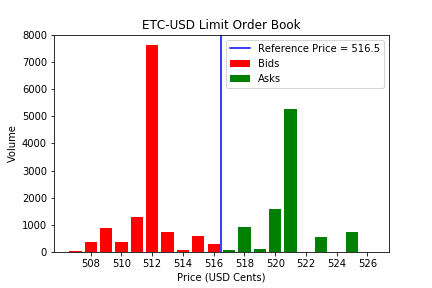
\includegraphics[width=0.8\textwidth]{Figures/12_30_18_LOB.png}
\label{fig:12_30_18_LOB_pic}
\end{center}
\end{figure}

This LOB is typical for ETC-USD, with most of the positions near the reference price filled. The bid and ask sides are relatively balanced, meaning that the reference price is stable. This is not always the case, as the bid or ask side could have significantly more volume when the price shifts. An sample of updates are shown in Figure \ref{fig:12_30_18_Updates}. Updates consist of the side, price, amount, and time. An update with an amount ``0" means that the volume at the price is completely consumed. As can be seen, the updates are given to the nearest millisecond and the majority of the updates occur near the reference price. The remainder of the thesis is based on the analysis of trading data from December 28-30, 2018 that includes almost all the trades of ETC-USD in that time period (with small gaps of a few minutes due to restarting data collection).

\begin{figure}[t]
\begin{center}
\caption{First 20 LOB Updates for December 30, 2018}
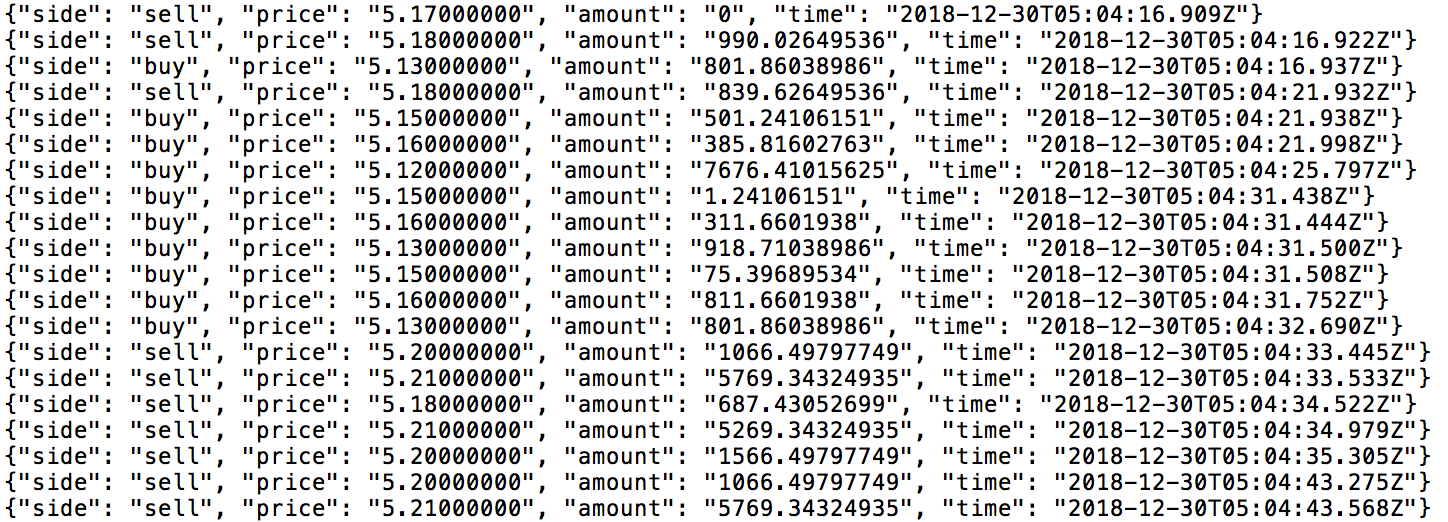
\includegraphics[width=0.8\textwidth]{Figures/12_30_18_Updates.png}
\label{fig:12_30_18_Updates}
\end{center}
\end{figure}




\chapter{Modelling the LOB}\label{ch:experiment}
\section{The Modified Queuing Model}\label{ch:queue_model}
Using the data collected, a model for simulating the LOB is created. It is based on the one developed by \cite{A6} but with several important modifications. The LOB is again represented as a $2K$-dimensional vector $$Q(t) = (Q_{-K}(t), \ldots Q_{-1}(t), Q_1(t), \ldots , Q_K(t))$$ centered around $p_0$. Events at each position $k$ cause either a positive or negative change in $Q_k(t)$. The magnitudes of the events are distributed exponentially with means $\mu^+_k$ and $\mu^-_k$ respectively. That is, if a positive event occurs at time $t$ with size $e$ at position $k$, set $q_k(t) \leftarrow q_k(t) + e$, and if a negative event occurs at time $t$ with size $e$ at position $k$, set $q_k(t) \leftarrow (q_k(t) - e)^+$ where $b^+ = 0$ if $b < 0$ and $b$ otherwise (in order to keep the queue size non-negative). An exception occurs when a negative event occurs at the best bid or ask price. It is assumed to be a market order that will consume liquidity from successive prices until it is filled. If the size of the event is larger than the volume at the best price, the leftover part of the order is filled with the next best price and so on. The arrivals of events are modelled as a multivariate Poisson process. With positive and negative arrivals at each of the $2K$ positions, there are $4K$ such processes. The marginal arrival process at each position is a Poisson process with positive and negative arrivals having mean rates $\lambda^+_k$ and $\lambda^-_k$ respectively. Arrivals are simulated in chunks of length $t$. Let $N^+_k(t)$ be the number of positive arrivals and $N^-_k(t)$ be the number of negative arrivals at position $k$ during a time period of length $t$. Then, the arrivals have a $4K\times4K$ correlation matrix $R$ where $R_{i+,j+} = corr(N^+_i(t), N^+_j(t))$, $R_{i+,j-} = corr(N^+_i(t), N^-_j(t))$, $R_{i-,j+} = corr(N^-_i(t), N^+_j(t))$, and $R_{i-,j-} = corr(N^-_i(t), N^-_j(t))$.

There are several differences between this model and the queue-reactive model developed by \cite{A6}. Modifications were made to better fit observations from the data set. First, the sizes of positive and negative events are not just the $AES$'s, but rather exponential random variables with means equal to the $AES$'s. This adjustment was made because the event sizes exhibit considerable variation. Section \ref{ch:event_sizes} shows that the exponential distribution reasonably fits the distributions of event sizes. Although it may not fit the data completely, it is the easiest part of the model to adjust.

Second, the rate of arrival of events at a given position does not vary as the size of the queue changes. In the data set, the queue sizes varied widely (sometimes several dozens multiplies of the $AES$'s) and no substantial changes in rates were observed when the queue sizes changed. It is possible that the rates differ in a predictable way as the queue sizes change, but there were not enough data points to observe reliable differences, especially in intermediate sizes where there was no data at all. This change also has the added benefit of simplifying the model greatly.

Third, arrival processes are modelled as a multivariate Poisson process instead of independent Poisson processes. In Section \ref{ch:poisson}, the claim that the arrival rates at each position reasonably follow individual Poisson processes is validated. However, Section \ref{ch:correlations} finds that these processes are significantly correlated. A multivariate Poisson process allows these correlations to be incorporated in the simulation.

\section{Building An Abbreviated Order Book}
To facilitate analysis, steps were taken to clean the raw data. Often in the data set, several updates that have the same magnitude, sign, and inter-arrival time occur in quick succession. These orders were likely made by a trader who split up a larger trade. As it should represent one event, orders that occur in quick succession (defined as occurring less than 0.01 seconds after the last) are combined if they have the same price and sign. 

Although the full order book is maintained after each update, the queuing model only contains the first $K$ prices on the bid and ask sides closest to $p_0$. Therefore, the parameters are only estimated for these positions. $p_0$ is maintained the same way as described in Section $\ref{modelLOB}$. If it changes, the data recording process is restarted. Analysis in the rest of the thesis is conducted for $K=10$, which is wide enough to include the vast majority of events. See Listing \ref{data-processing-code} for the code written to process the data and build the abbreviated order book.

\section{Event Size Estimates}\label{ch:event_sizes}
The sizes of the events at position $k$ are distributed exponentially with means $\mu^+_k$ and $\mu^-_k$. A reasonable choice for $\mu^+_k$ and $\mu^-_k$ is the $AES$ for positive and negative events at each $k$. This section examines whether the event sizes can reasonably fitted with exponential distributions with rates equal to the $AES$'s. 

\begin{figure}
\centering
\caption{Event Sizes Compared to Exponential Distribution (4 Positions Closest to $p_0$)}
\begin{tabular}{cc}
\hline
\subf{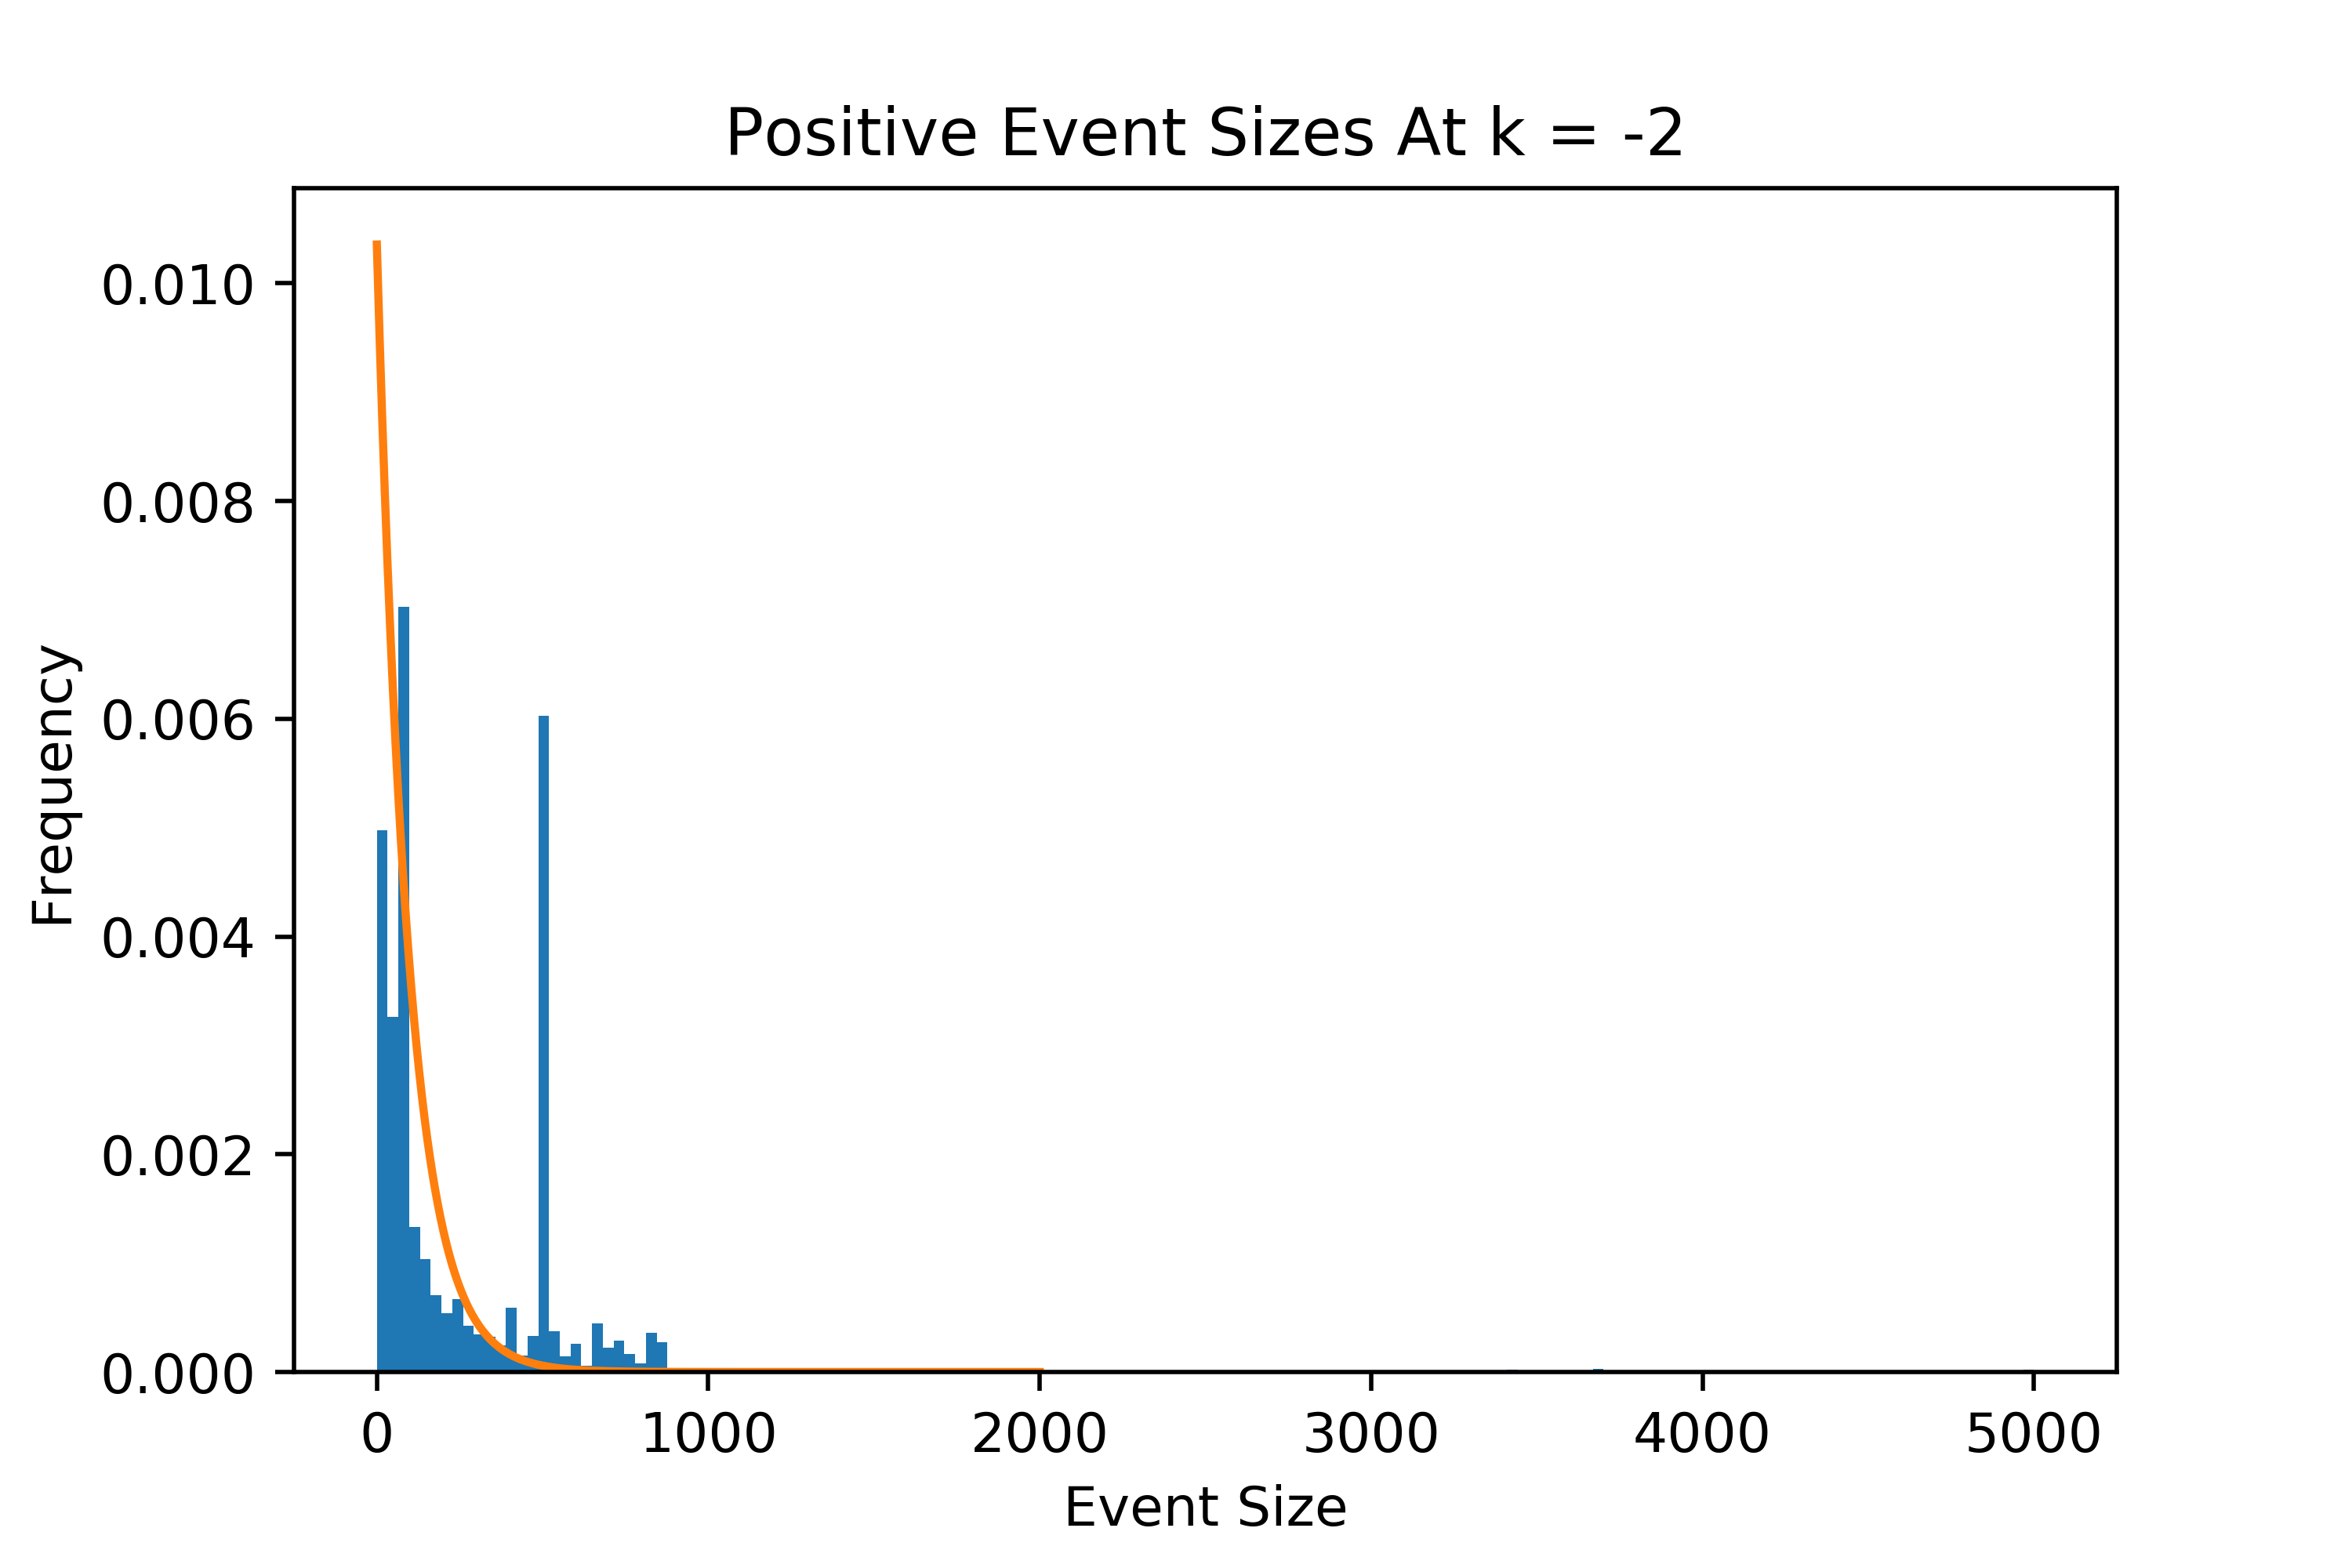
\includegraphics[width=60mm]{Figures/pos_-2.png}}
{}
&
\subf{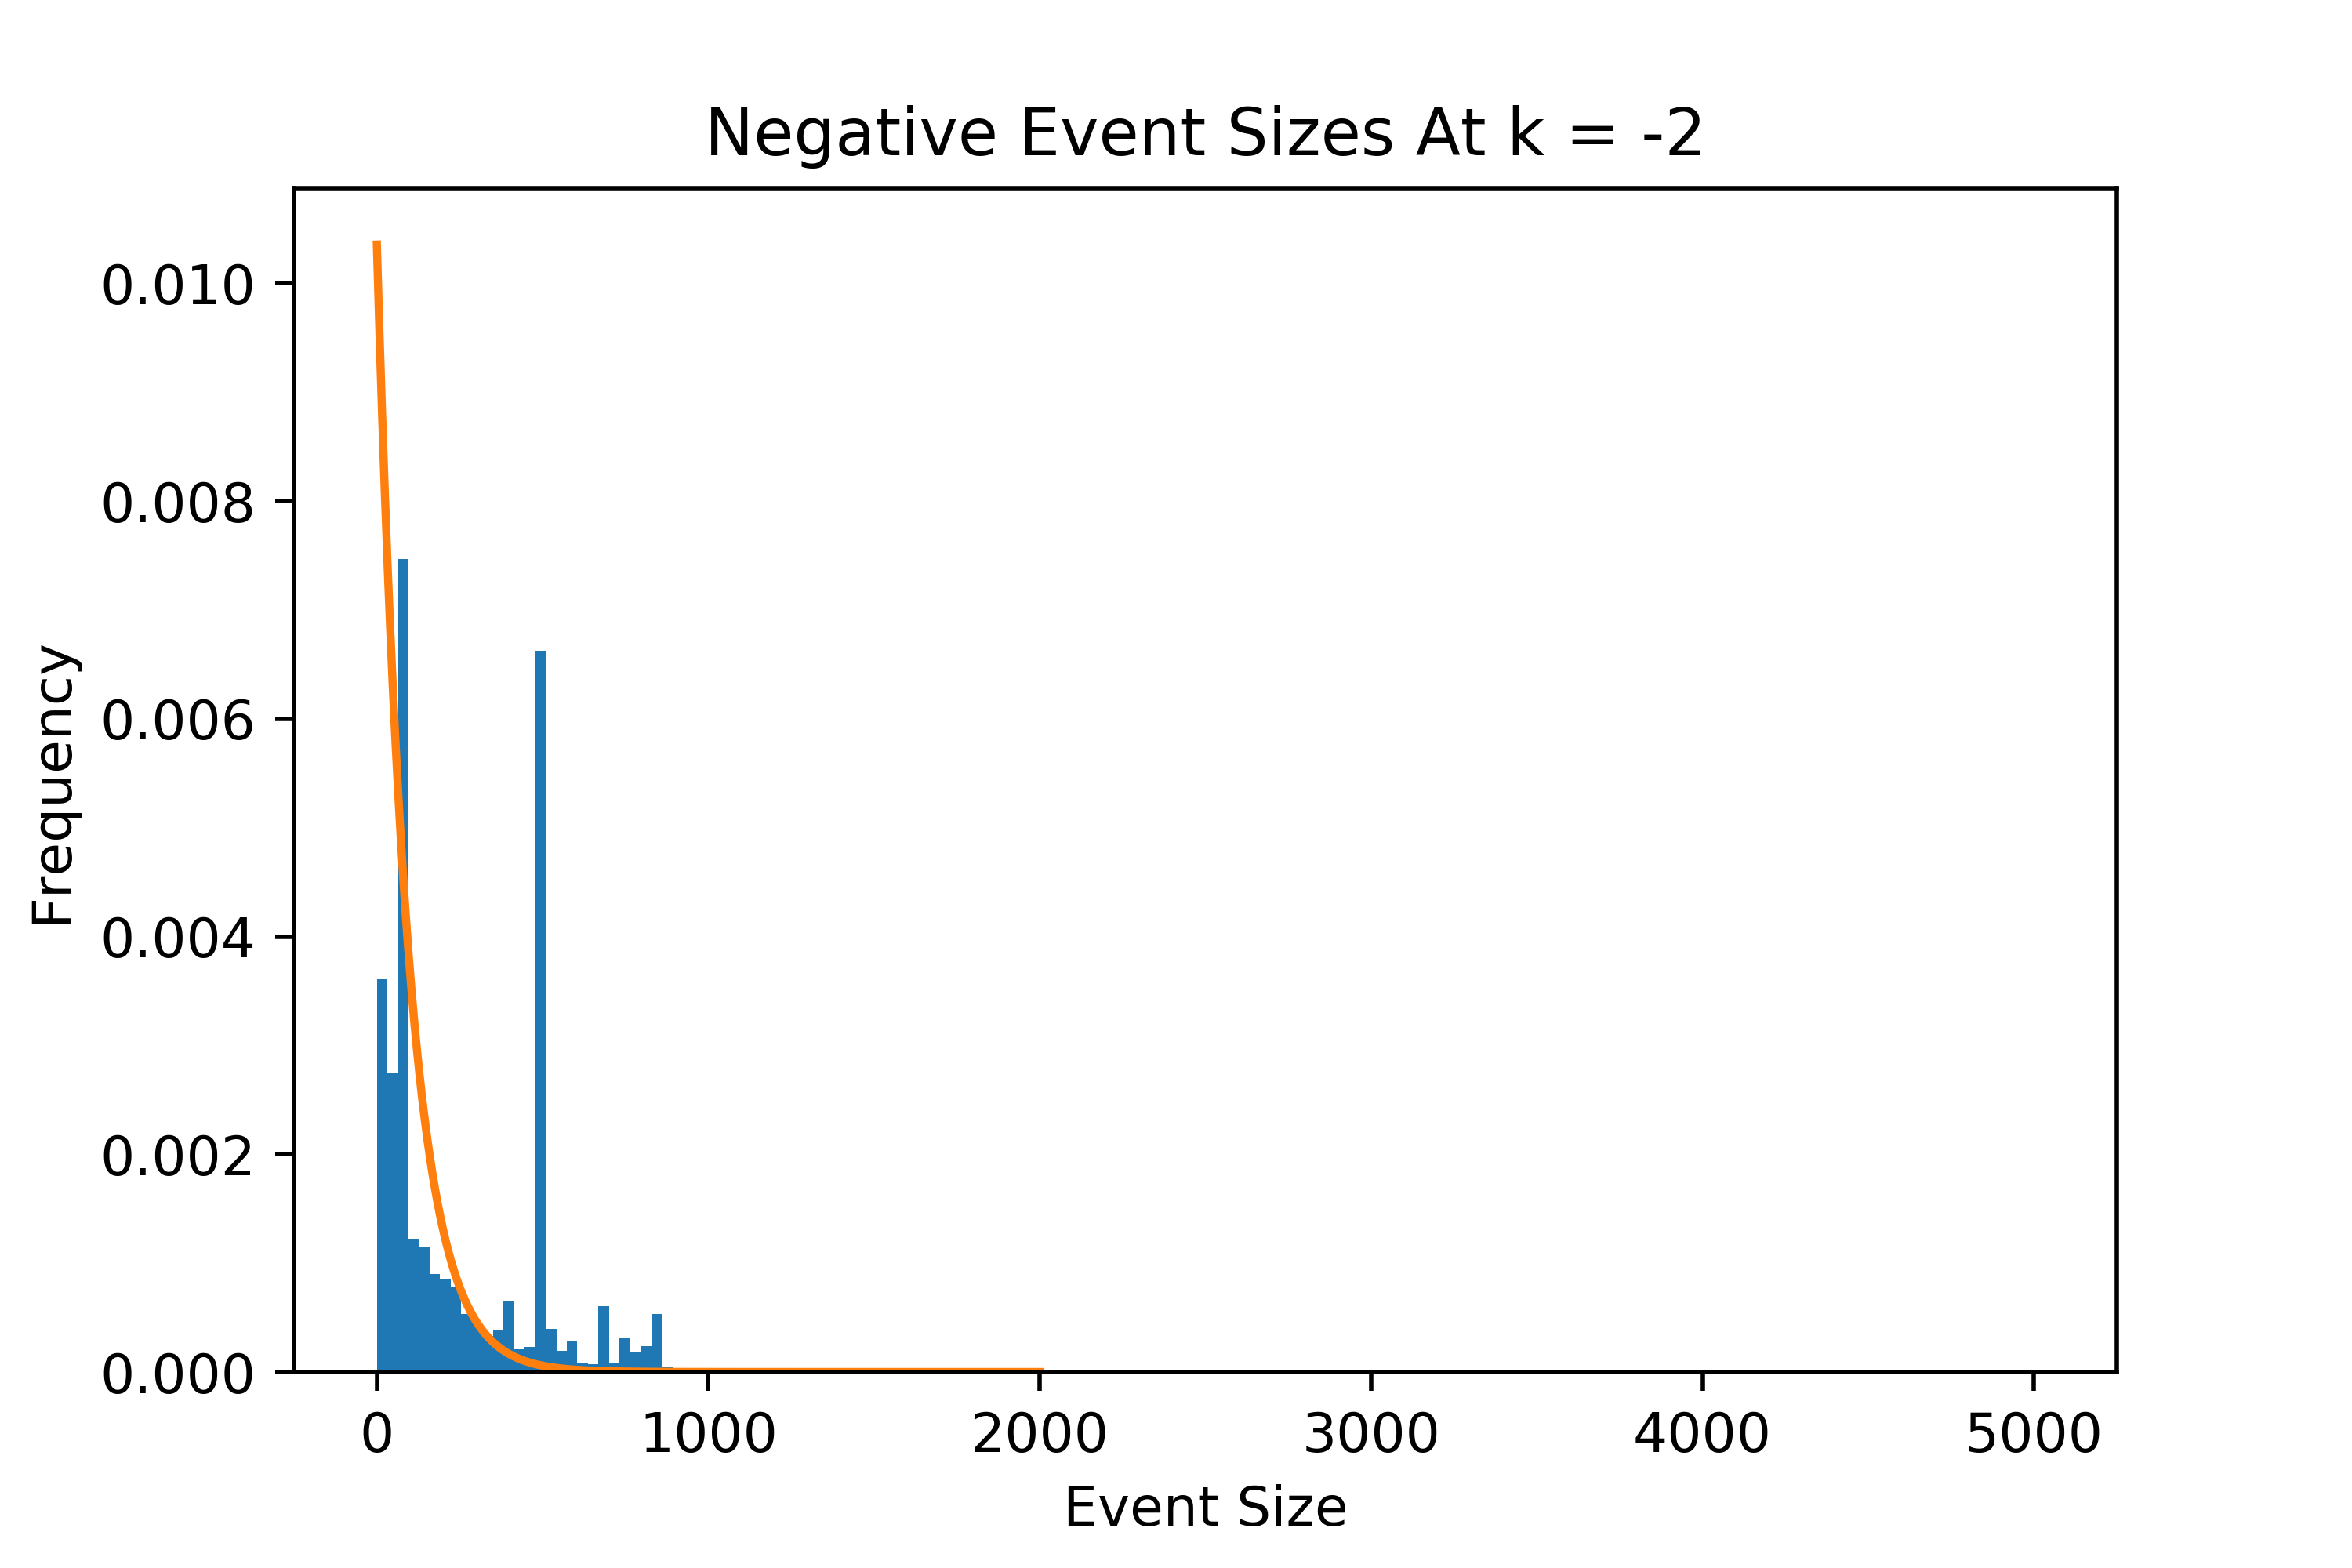
\includegraphics[width=60mm]{Figures/neg_-2.png}}
{}
\\
\subf{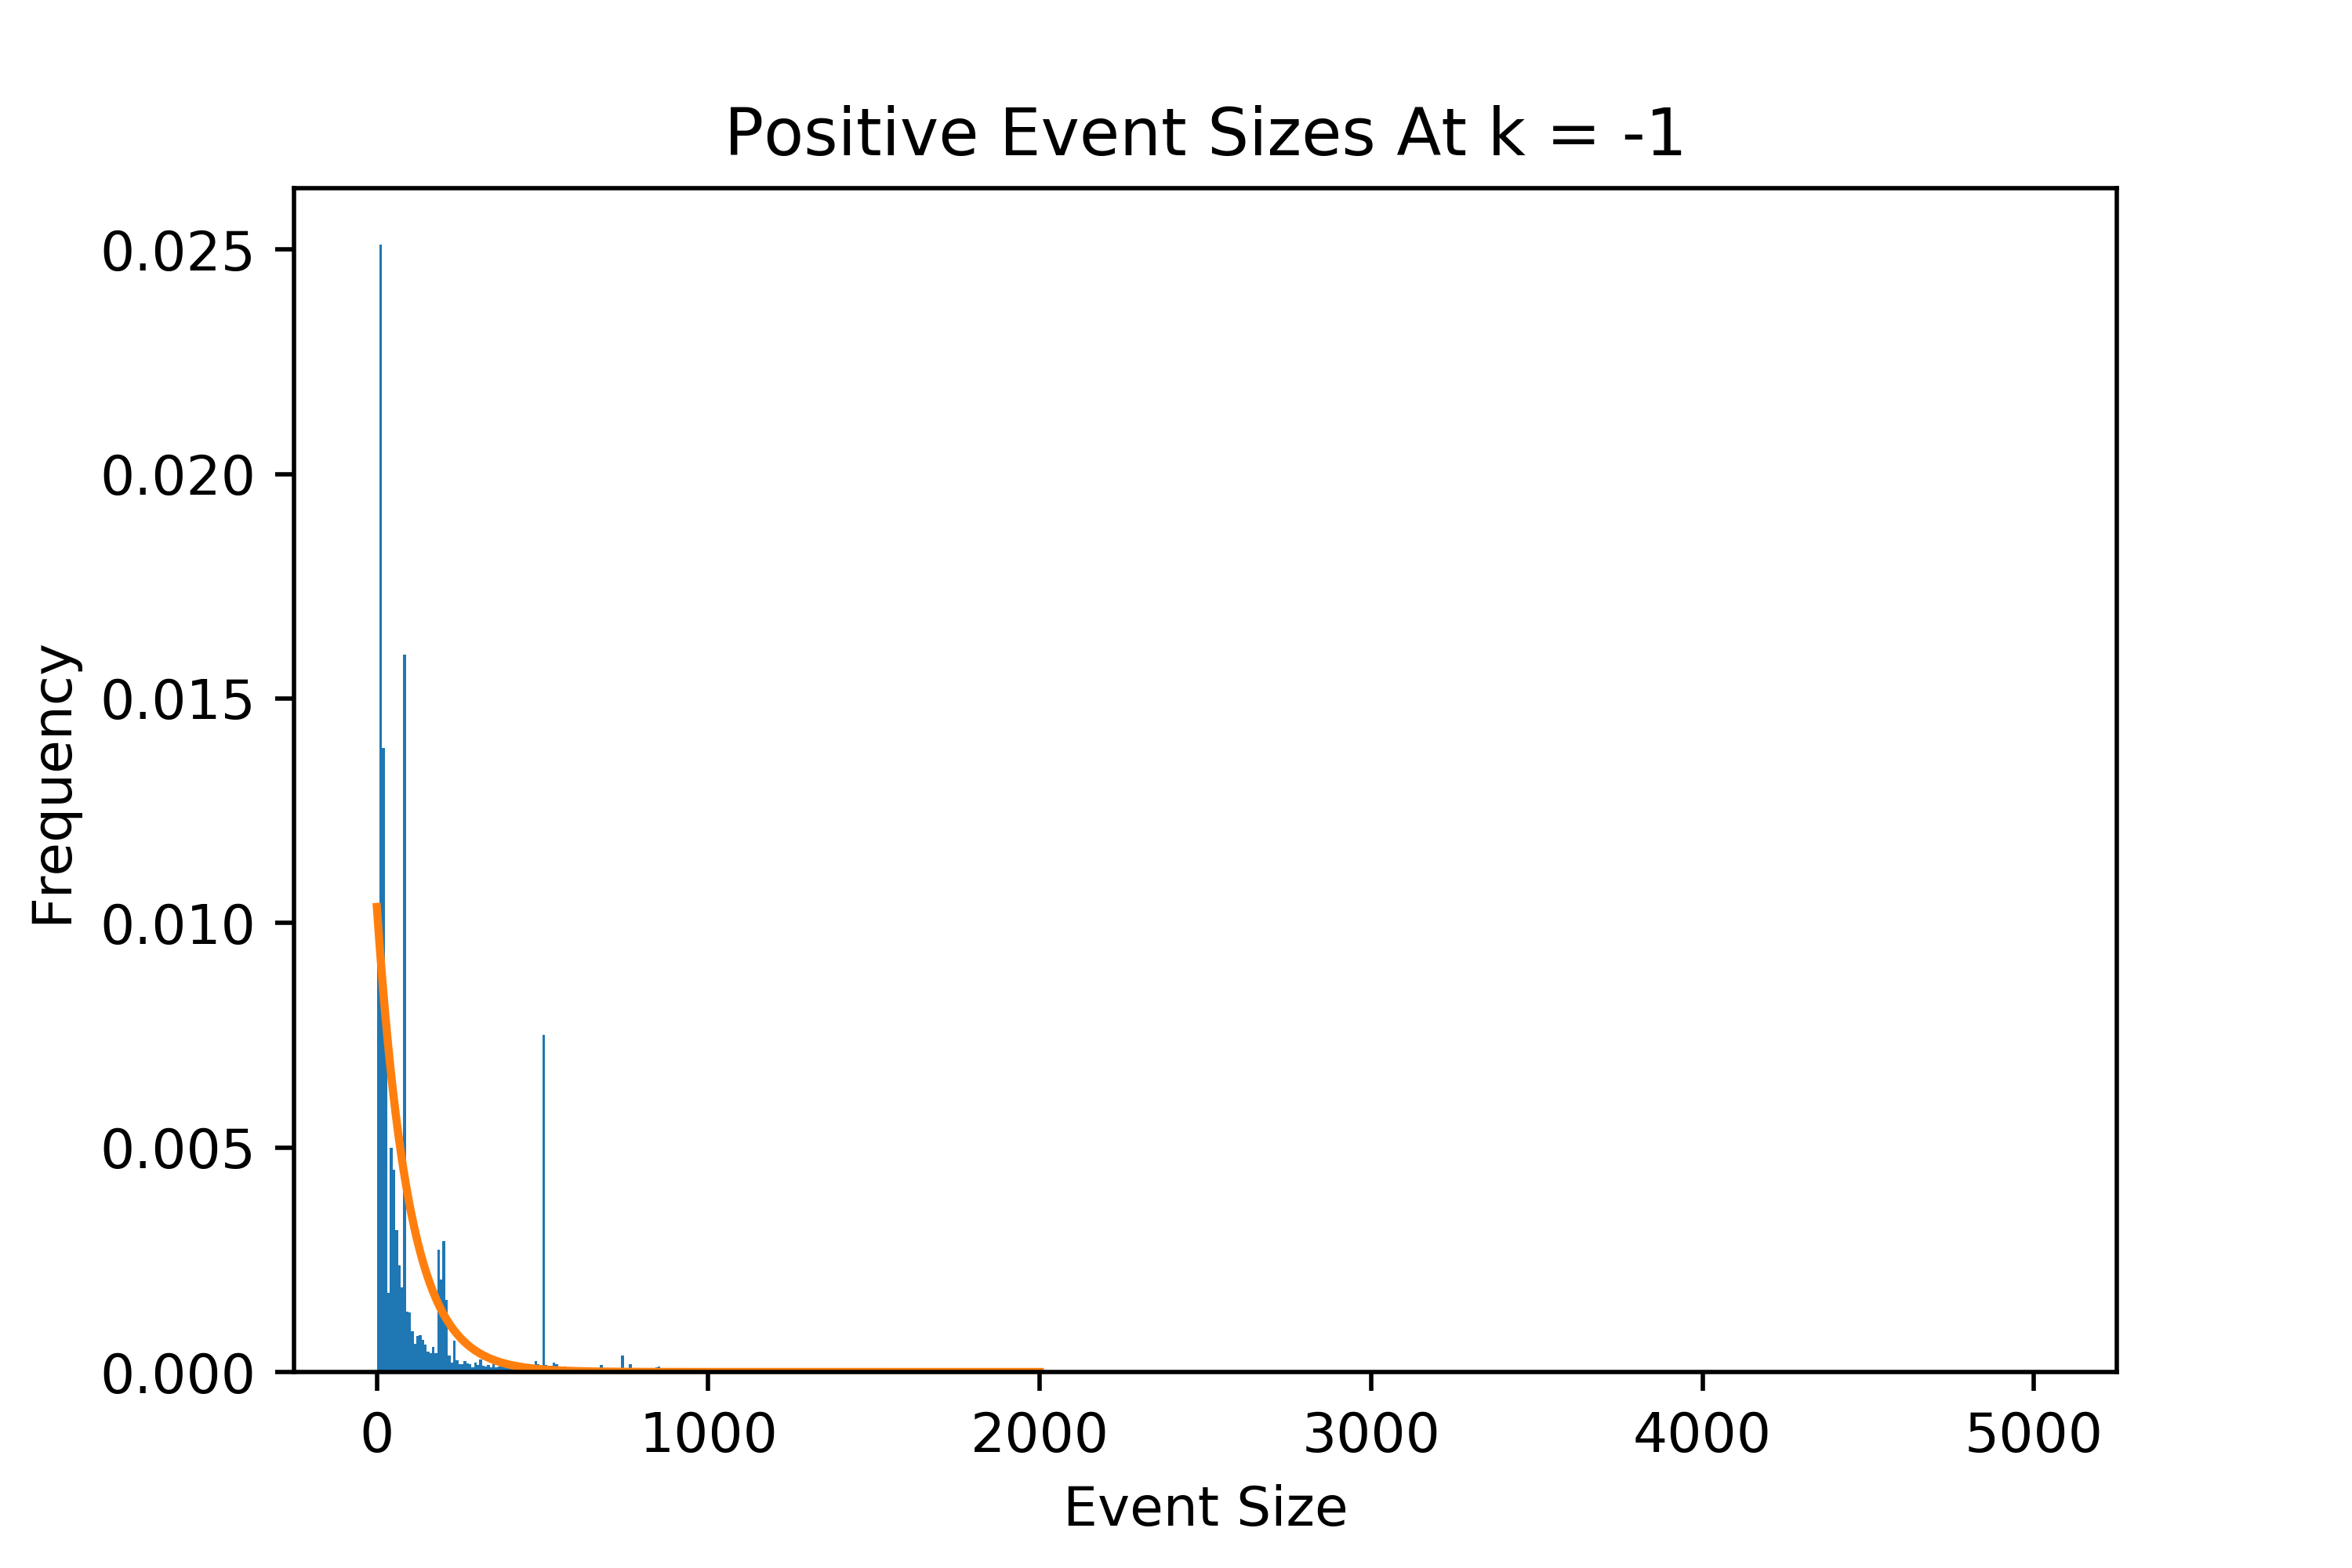
\includegraphics[width=60mm]{Figures/pos_-1.png}}
{}
&
\subf{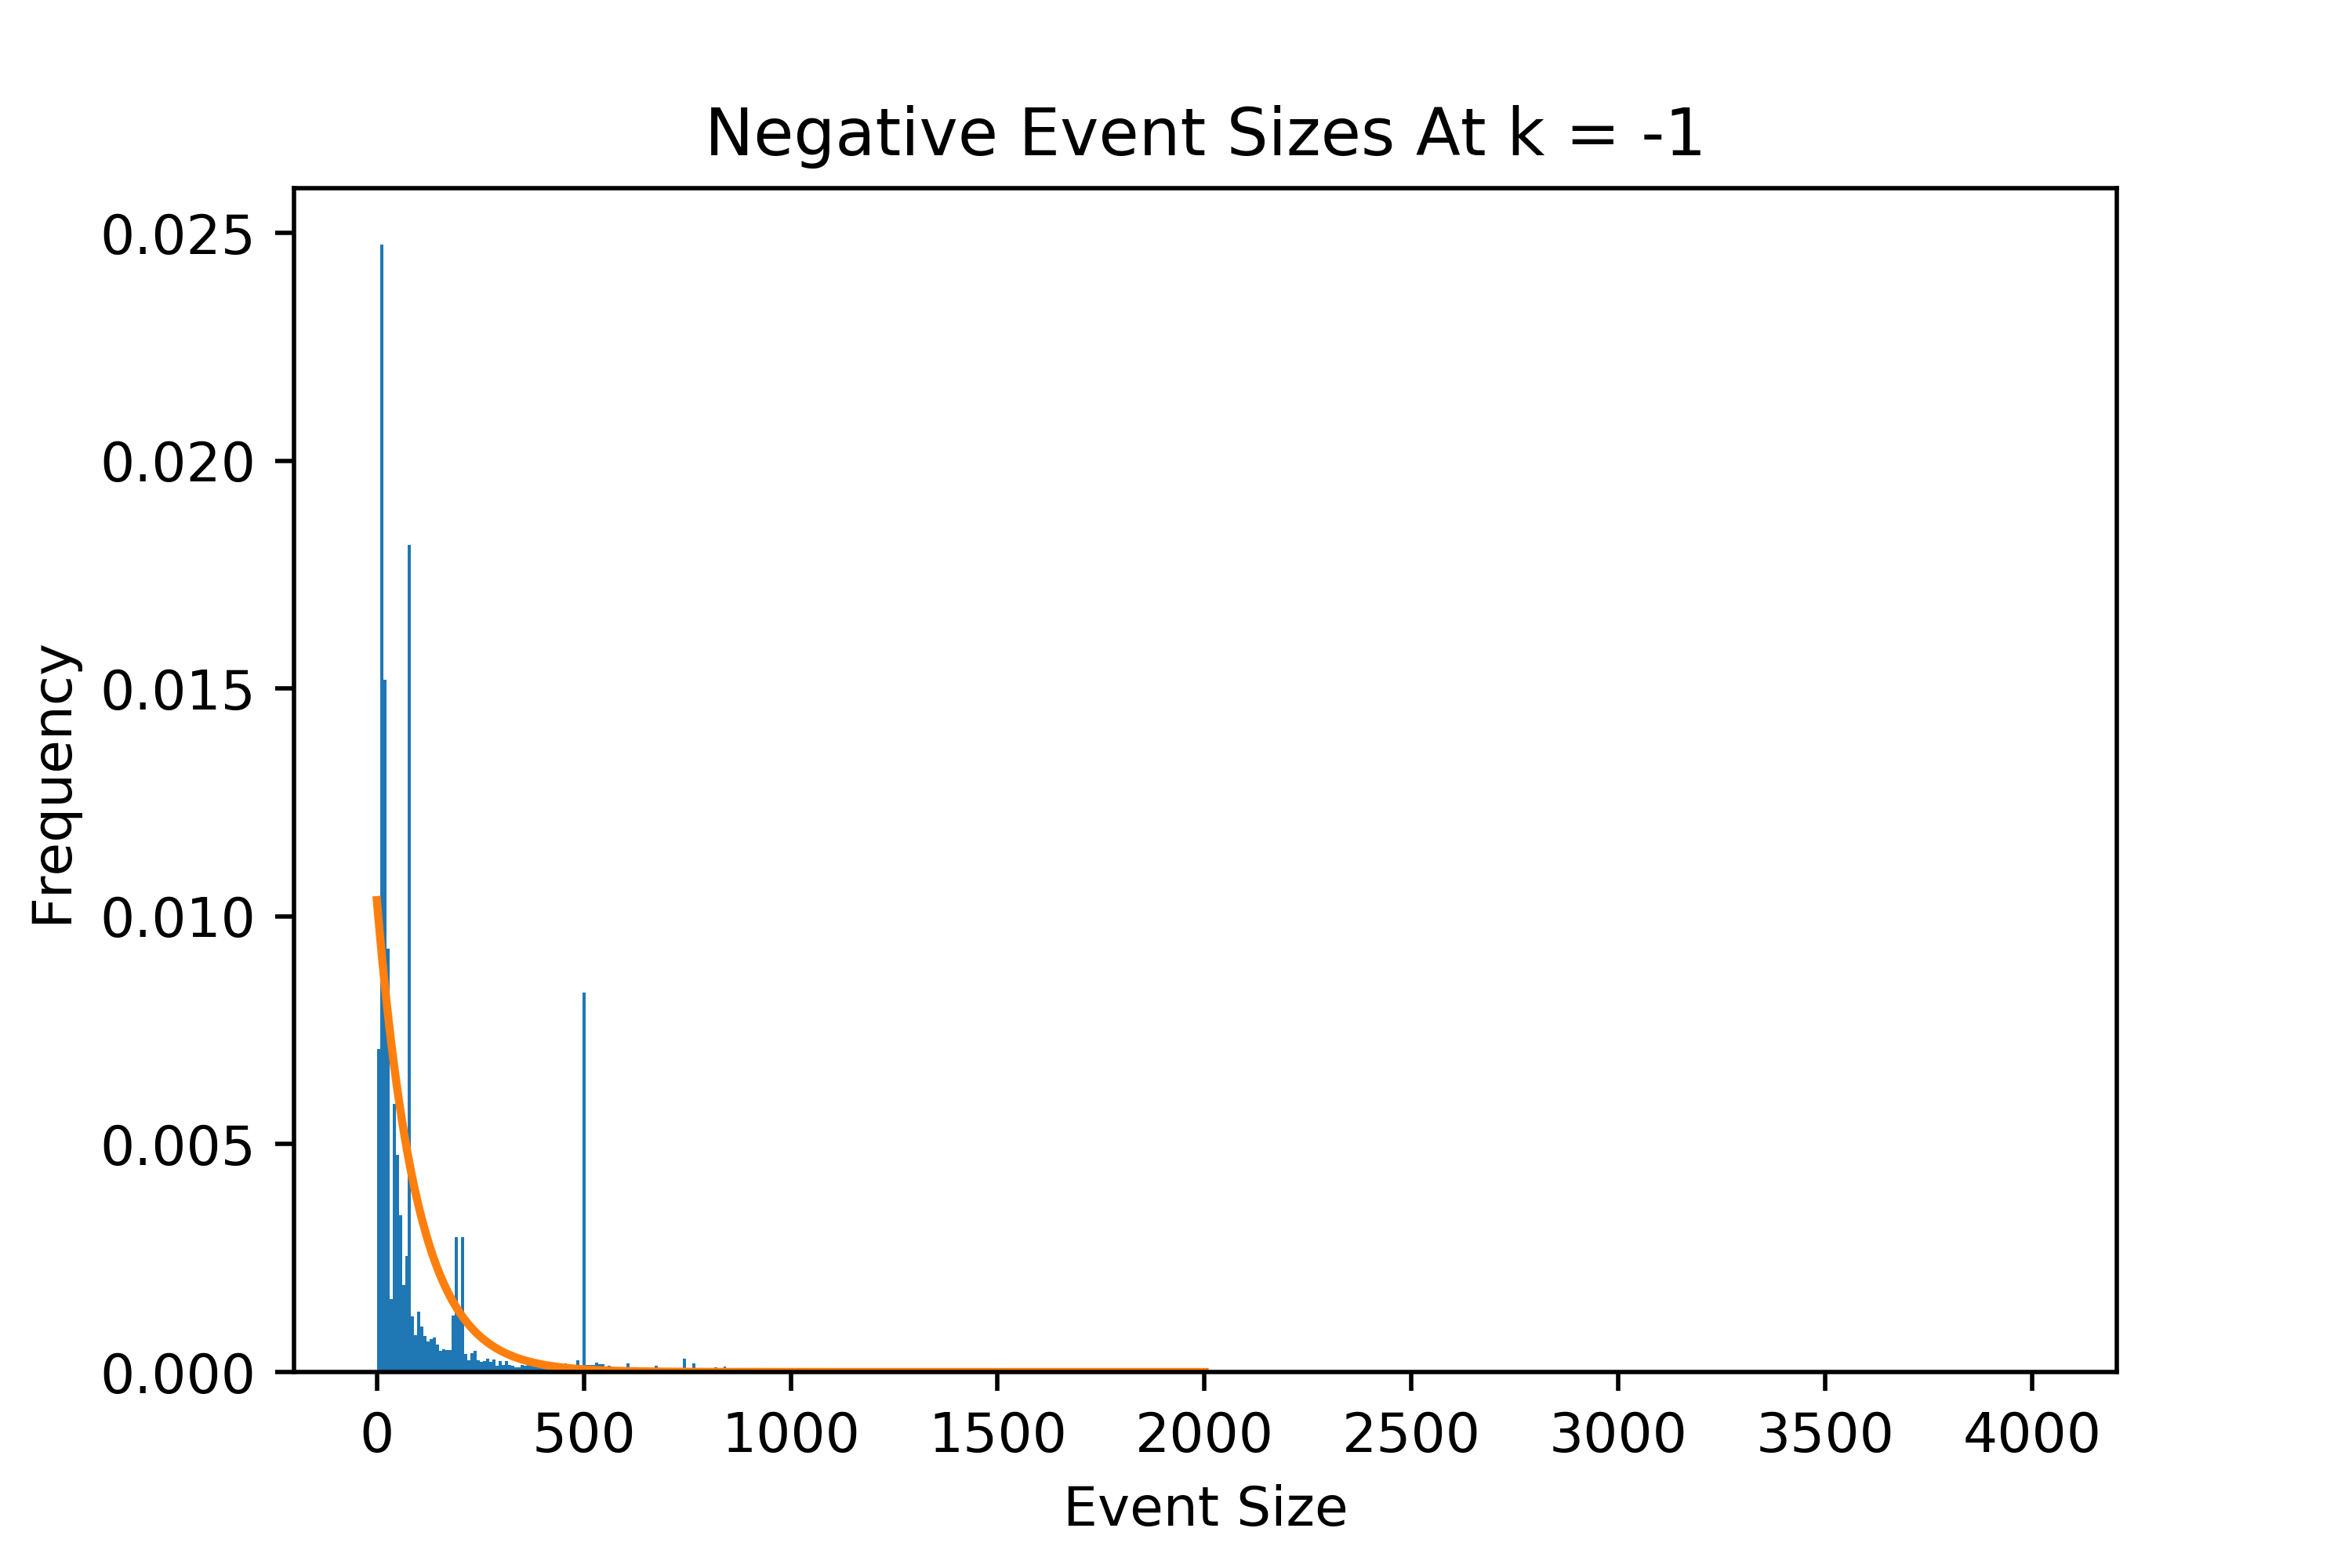
\includegraphics[width=60mm]{Figures/neg_-1.png}}
{}
\\
\subf{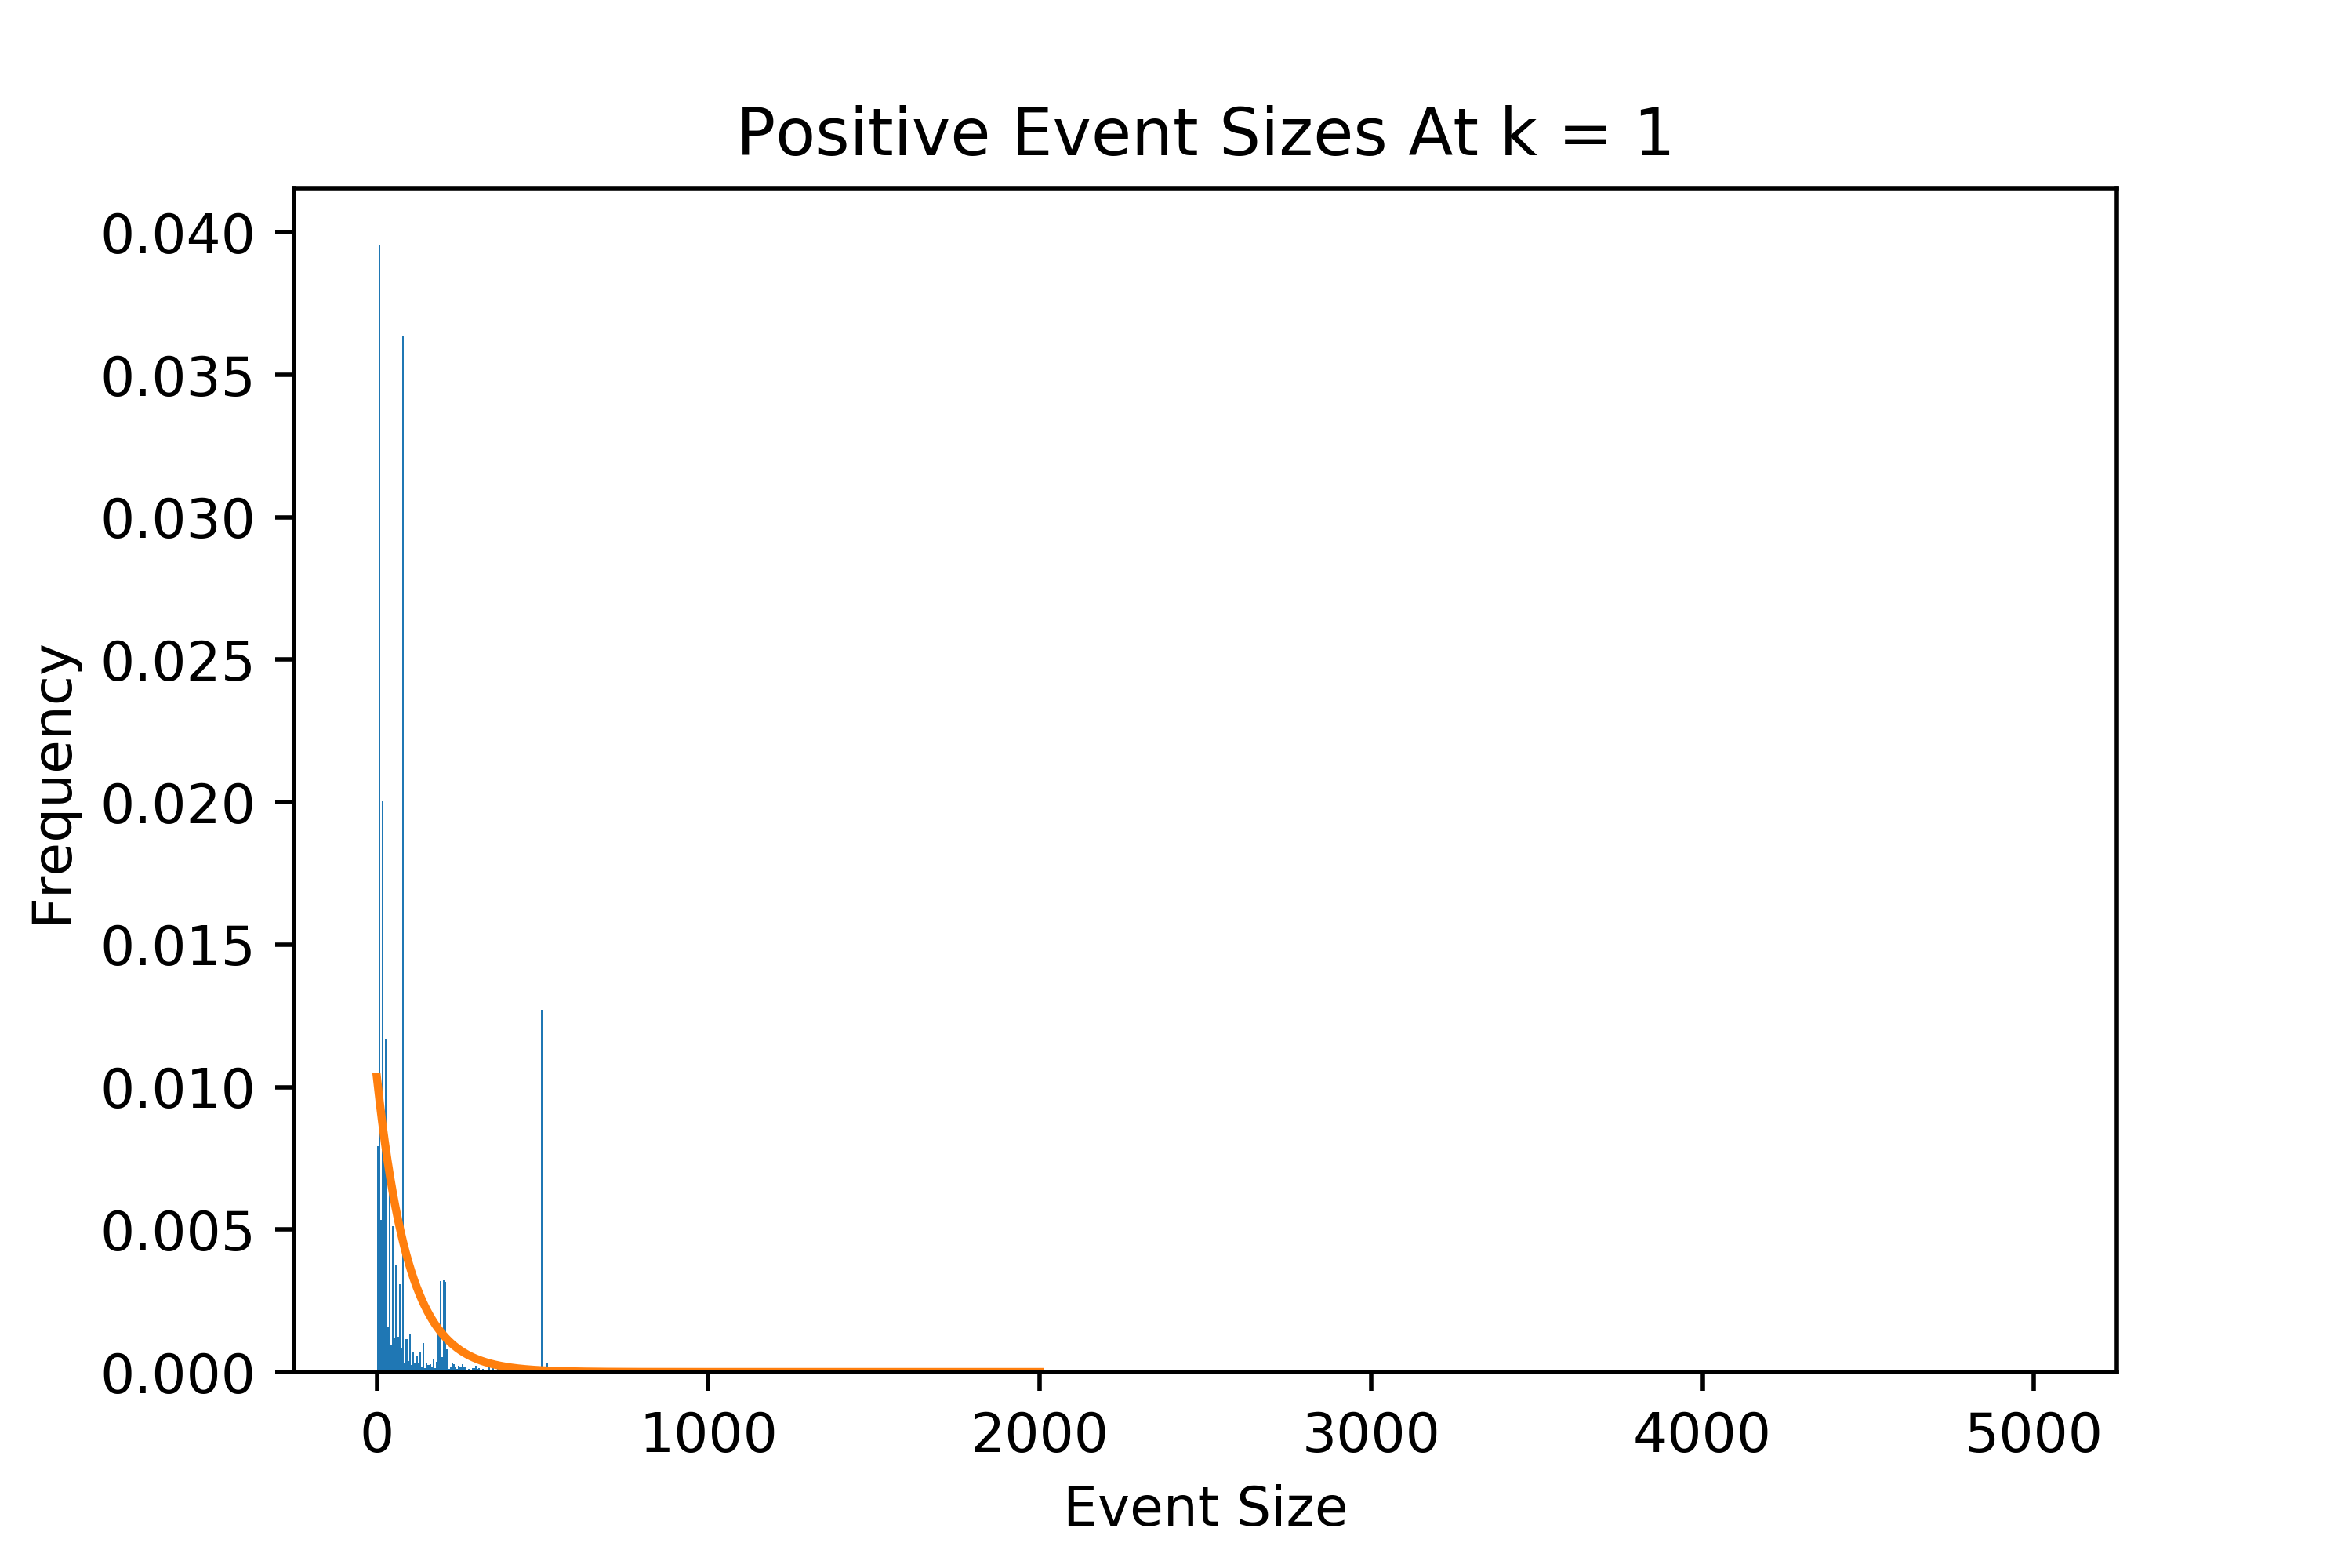
\includegraphics[width=60mm]{Figures/pos_1.png}}
{}
&
\subf{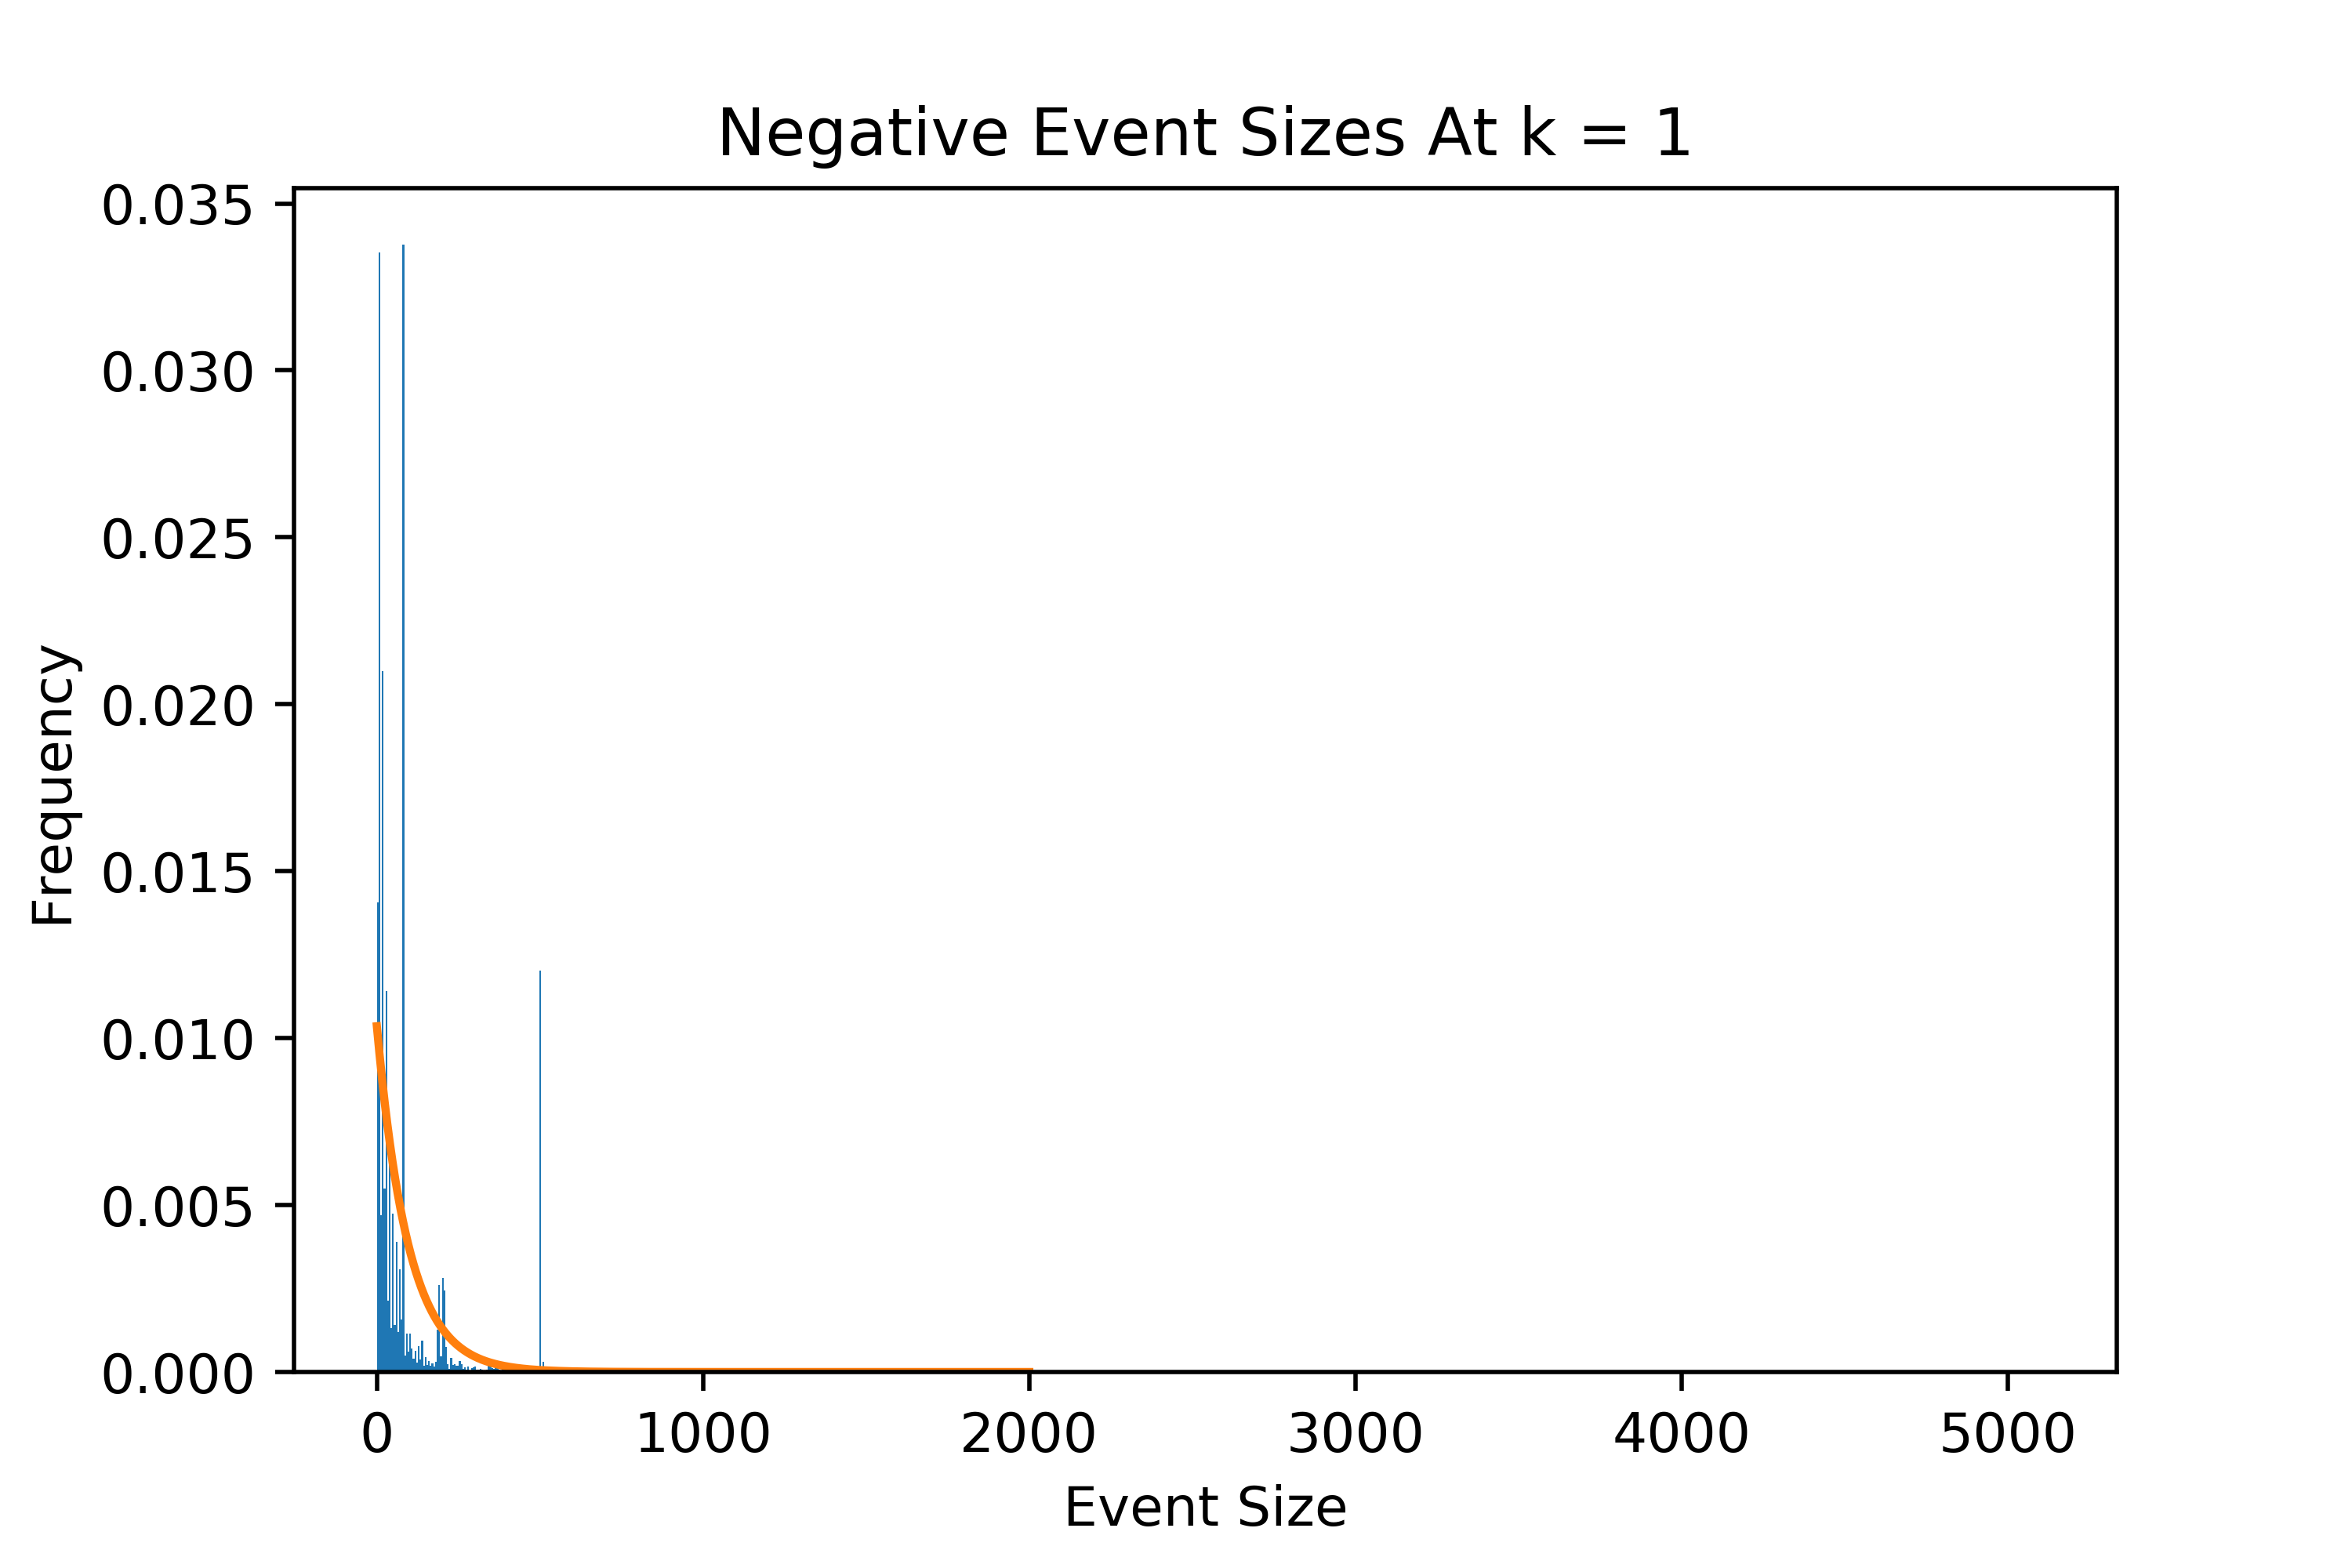
\includegraphics[width=60mm]{Figures/neg_1.png}}
{}
\\
\subf{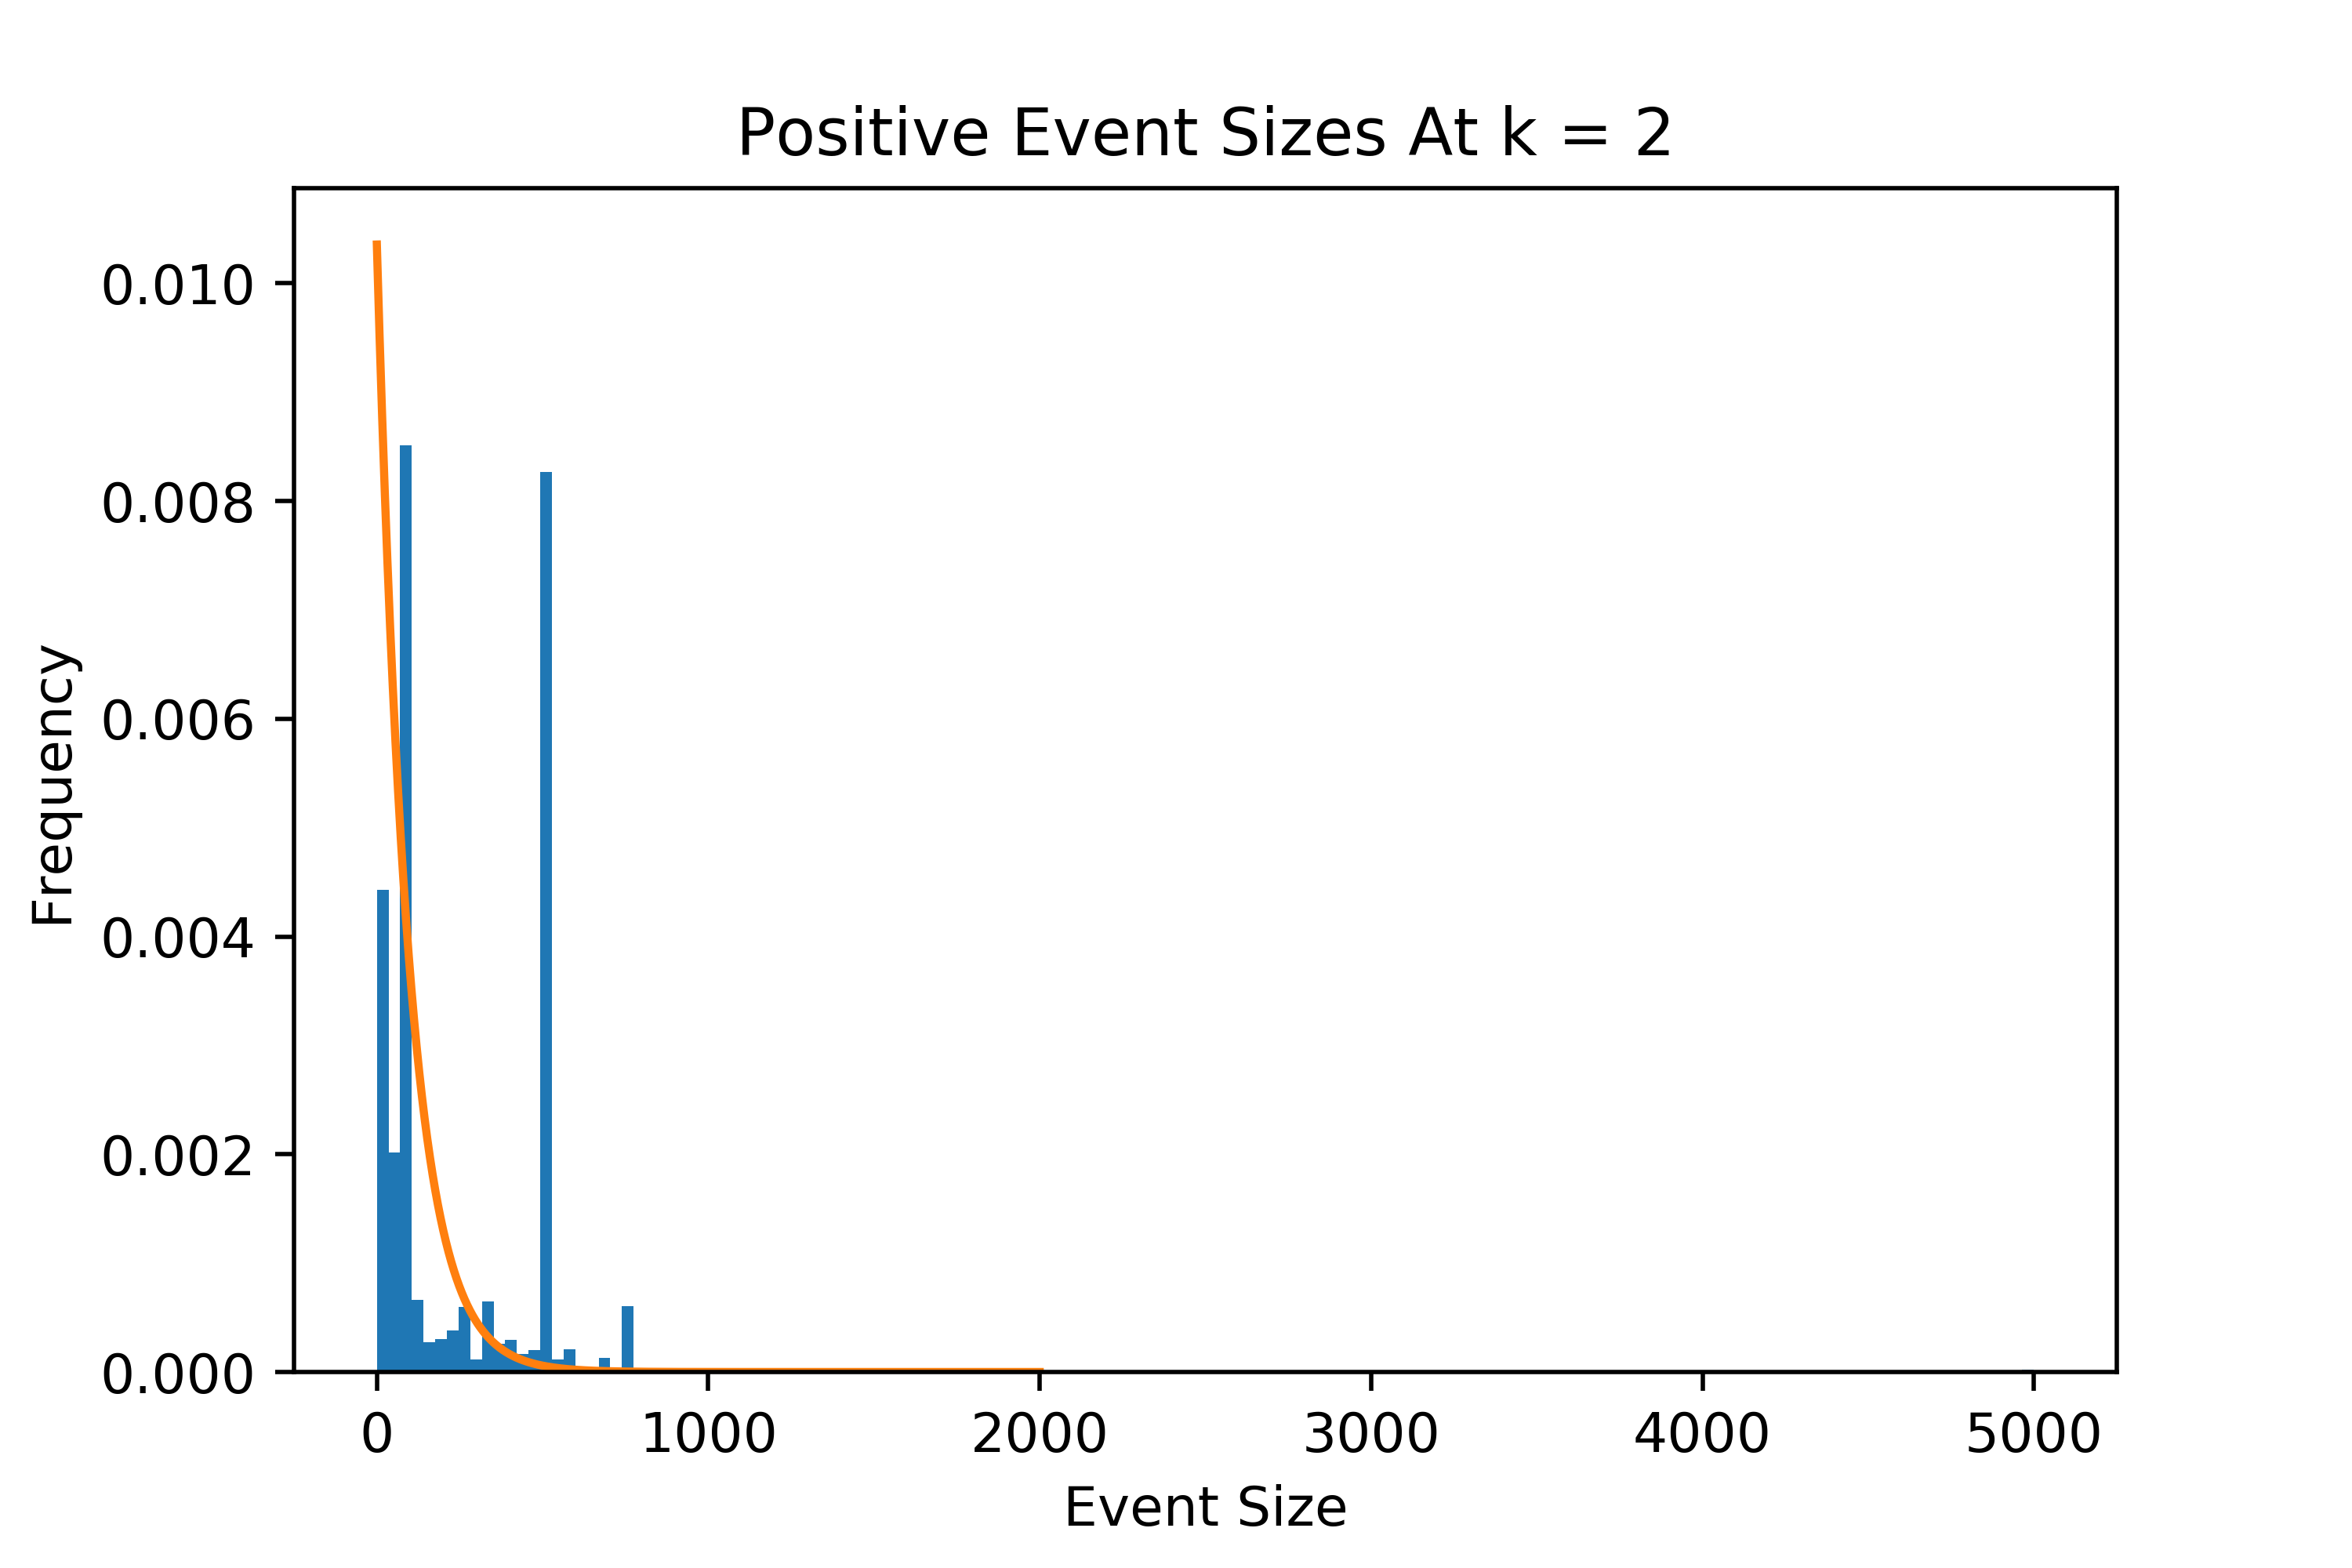
\includegraphics[width=60mm]{Figures/pos_2.png}}
{}
&
\subf{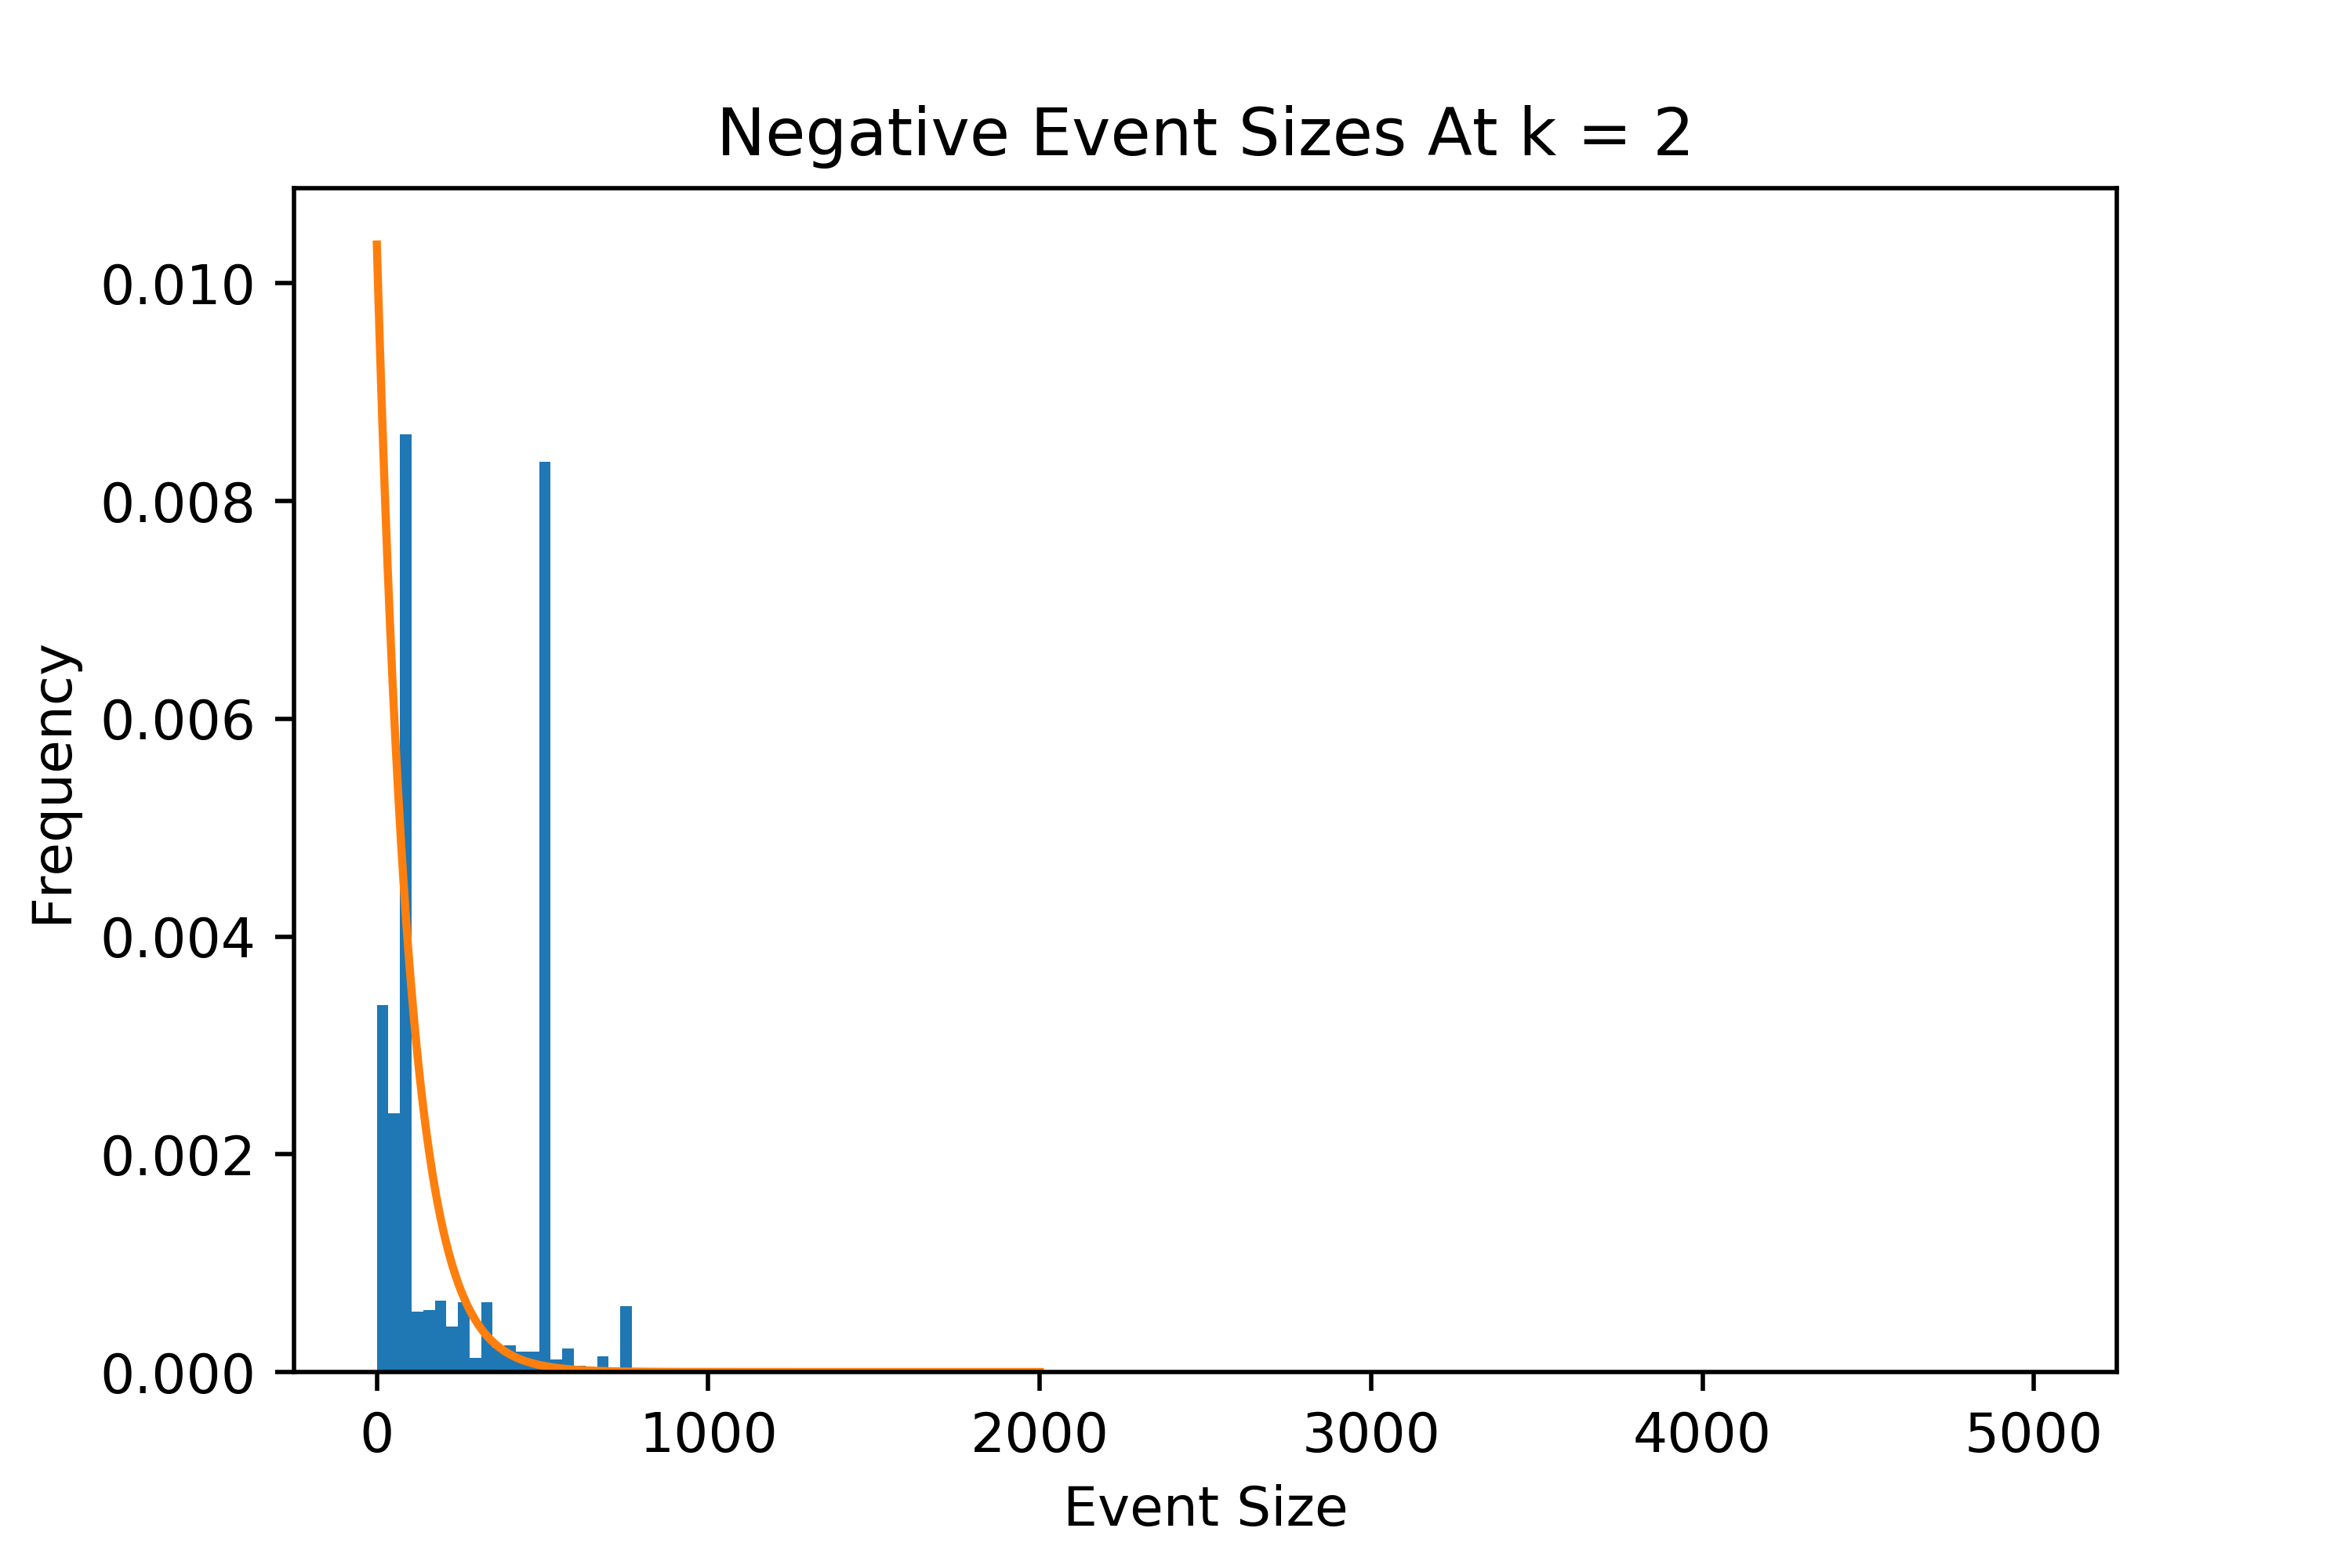
\includegraphics[width=60mm]{Figures/neg_2.png}}
{}
\\
\hline
\end{tabular}
\label{fig:sizes}
\end{figure}

Histograms of event sizes at each position are shown in Figure \ref{fig:sizes}. Exponential distributions with means equal to the $AES$'s are overlaid on top. As can be seen, the exponential distributions fit the histograms relatively well. However, there are some notable discrepancies. One is the high frequency of orders of size 500. A possible explanation for this observation is that 500 may be a common size used by traders to split up large orders. There are also a non-negligible number of orders near 5000, since that is the upper limit order size imposed by Coinbase. Although it may be possible to more accurately model the dynamics of the ETC-USD LOB with these characteristics taken into account, they are not included in the model so that it can be more broadly applicable to other securities. The $AES$'s are listed in Table \ref{tab:parameters} as $\mu^{\pm}_k$. See Listing \ref{AES_and_rate_code} for the code used to find the $AES$'s. It can be seen that in general, as the price gets closer to $p_0$, $\mu_k^{\pm}$ decreases, but the number of events across the time period, $n^{\pm}_k$, increases. This higher rate of activity near $p_0$ makes sense, since market orders are executed at the best available prices and market makers are incentivized by the fee structure to provide liquidity around $p_0$.

\begin{table}[htbp]
\caption{Event Size and Arrival Rate Parameter Estimates} \label{tab:parameters}
\begin{center}
\begin{tabular}{l|llll|llll}
\hline \hline
 & \multicolumn{4}{l|}{\textbf{Positive Events}} & \multicolumn{4}{l}{\textbf{Negative Events}} \\
\hline
$k$   & $n_k^+$ & $\mu^+_k$ & $\lambda^+_k$ & $\mu^+_k \cdot \lambda^+_k$ & $n_k^-$  & $\mu^-_k$  & $\lambda^-_k$ & $\mu^-_k \cdot \lambda^-_k$  \\
\hline
-10 & 406   & 601.41 & 0.0016 & 0.94      & 493   & 597.76 & 0.0019 & 1.14       \\
-9  & 699   & 479.69 & 0.0027 & 1.29      & 739   & 446.6  & 0.0029 & 1.27       \\
-8  & 1554  & 584.57 & 0.006  & 3.5       & 1602  & 552.68 & 0.0062 & 3.42       \\
-7  & 5633  & 530.34 & 0.0217 & 11.53     & 5417  & 534.07 & 0.0209 & 11.16      \\
-6  & 13115 & 520.95 & 0.0506 & 26.36     & 12852 & 531.86 & 0.0496 & 26.37      \\
-5  & 21824 & 487.88 & 0.0842 & 41.08     & 21850 & 494.66 & 0.0843 & 41.7       \\
-4  & 27620 & 427.19 & 0.1066 & 45.52     & 27578 & 433.09 & 0.1064 & 46.08      \\
-3  & 33187 & 368.47 & 0.128  & 47.18     & 33214 & 367.8  & 0.1281 & 47.13      \\
-2  & 47229 & 232.15 & 0.1822 & 42.3      & 45189 & 247.63 & 0.1743 & 43.17      \\
-1  & 54254 & 104.11 & 0.2093 & 21.79     & 49177 & 104.8  & 0.1897 & 19.88      \\
1   & 48246 & 93.79  & 0.1861 & 17.46     & 46787 & 89.82  & 0.1805 & 16.21      \\
2   & 37702 & 226.64 & 0.1455 & 32.96     & 38310 & 229.59 & 0.1478 & 33.93      \\
3   & 41409 & 305.04 & 0.1598 & 48.73     & 41912 & 302.37 & 0.1617 & 48.89      \\
4   & 44948 & 328.57 & 0.1734 & 56.98     & 44616 & 333.46 & 0.1721 & 57.4       \\
5   & 37880 & 318.37 & 0.1461 & 46.53     & 37105 & 325.12 & 0.1431 & 46.54      \\
6   & 16320 & 360.54 & 0.063  & 22.7      & 15669 & 375.32 & 0.0604 & 22.69      \\
7   & 3818  & 577.4  & 0.0147 & 8.5       & 3672  & 587.94 & 0.0142 & 8.33       \\
8   & 1271  & 599.09 & 0.0049 & 2.94      & 1280  & 516.85 & 0.0049 & 2.55       \\
9   & 602   & 428.87 & 0.0023 & 1         & 543   & 484.68 & 0.0021 & 1.02       \\
10  & 548   & 366.15 & 0.0021 & 0.77      & 529   & 370.48 & 0.002  & 0.76      
\end{tabular}
\end{center}
\end{table}

\section{Arrival Rate Estimates}\label{ch:poisson}
The event arrivals are modelled as a multivariate Poisson process, where the marginal processes at each position $k$ have average arrival rates $\lambda^{\pm}_k$. First, the claim that individual event arrivals at each position follow Poisson processes is examined. To do so, inter-arrival times of the events are tested to see if they are exponentially distributed. Figures \ref{fig:interarrivals_pos} and \ref{fig:interarrivals_neg} show QQ-plots and histograms of the inter-arrival times compared to exponential distributions. From the QQ-plots, it can be seen that the inter-arrival times have heavy right tails compared to the exponential distribution. From the histograms, it can be seen that the exponential distribution fits the data well for the majority of the data points except for a small number of points on the right that comprise the heavy tails. Because the exponential distribution reasonably fits the inter-arrival times as a whole, the arrivals are modelled as a multivariate Poisson process for its desirable properties in simulation. We estimate $\lambda^{\pm}_k$ by taking the number of arrivals of the specified event ($N^{\pm}_k$) divided by the total time period. The code used to find the rates is found in Listing \ref{AES_and_rate_code}. The average rates are reported in Table \ref{tab:parameters}.

\begin{figure}
\centering
\caption{Inter-Arrival Times for Positive Events Compared to Exponential Distribution (4 Positions Closest to $p_0$)}
\begin{tabular}{cc}
\hline
\subf{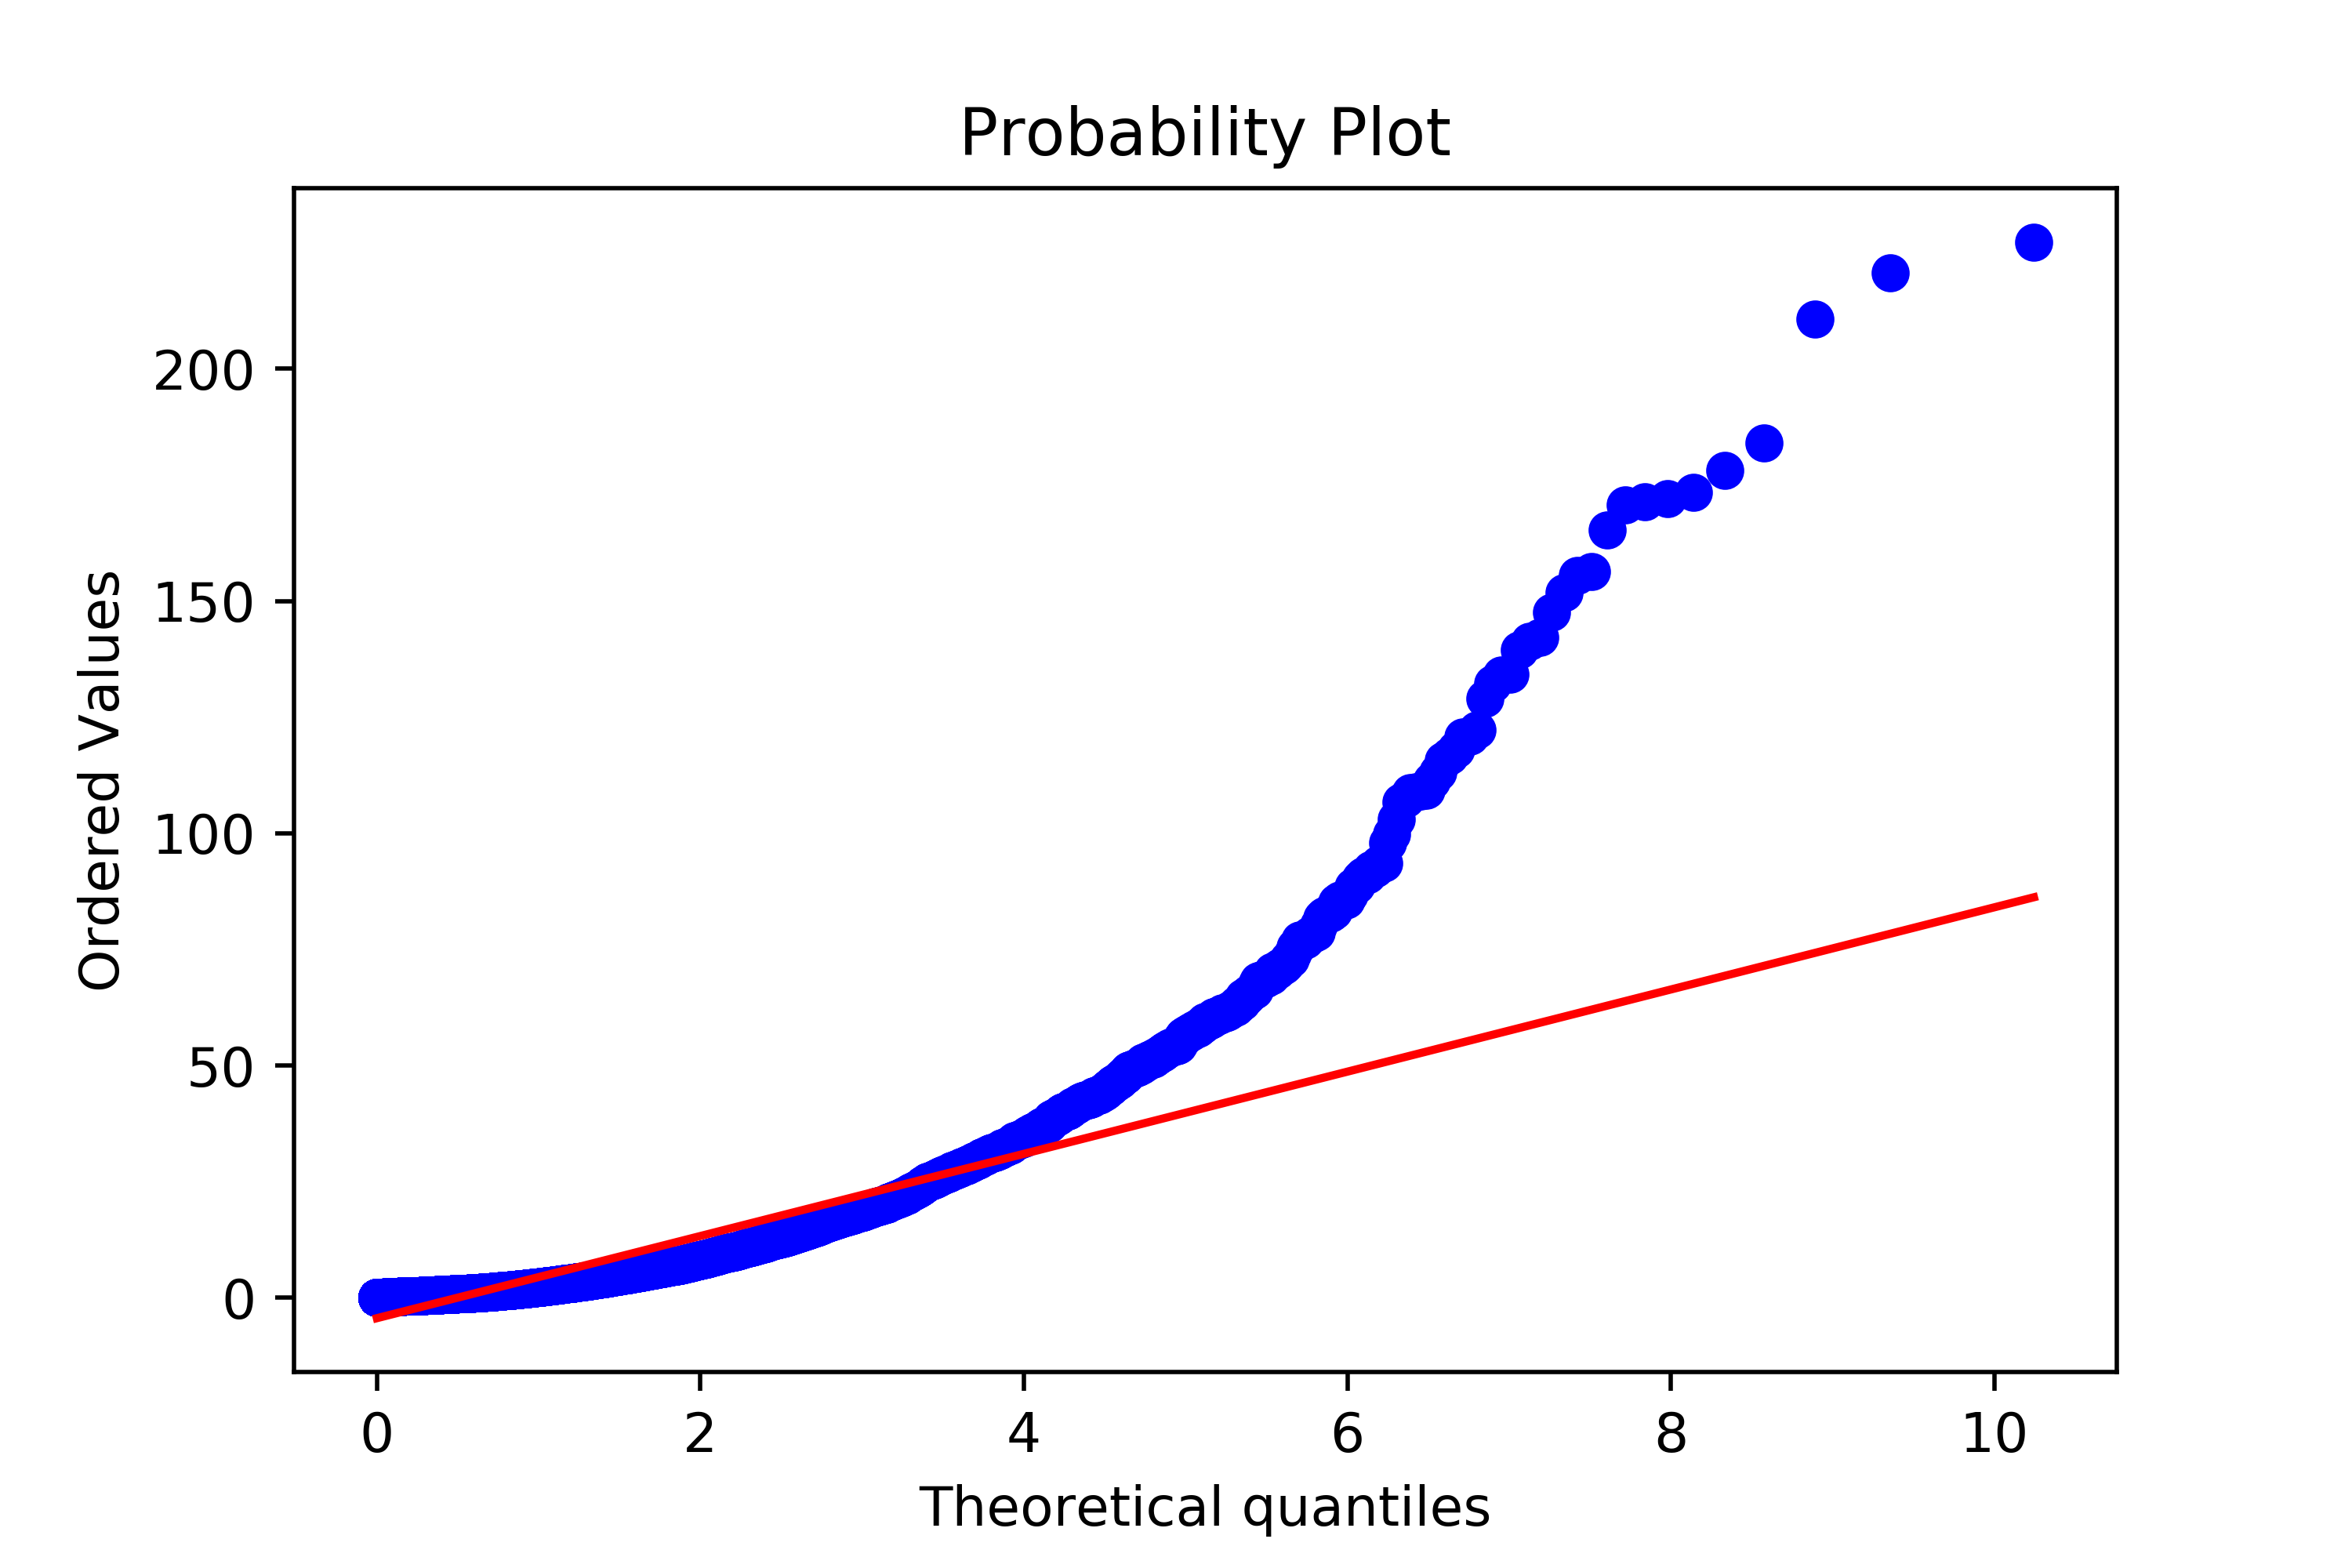
\includegraphics[width=60mm]{Figures/QQ_pos_k-2.png}}
{}
&
\subf{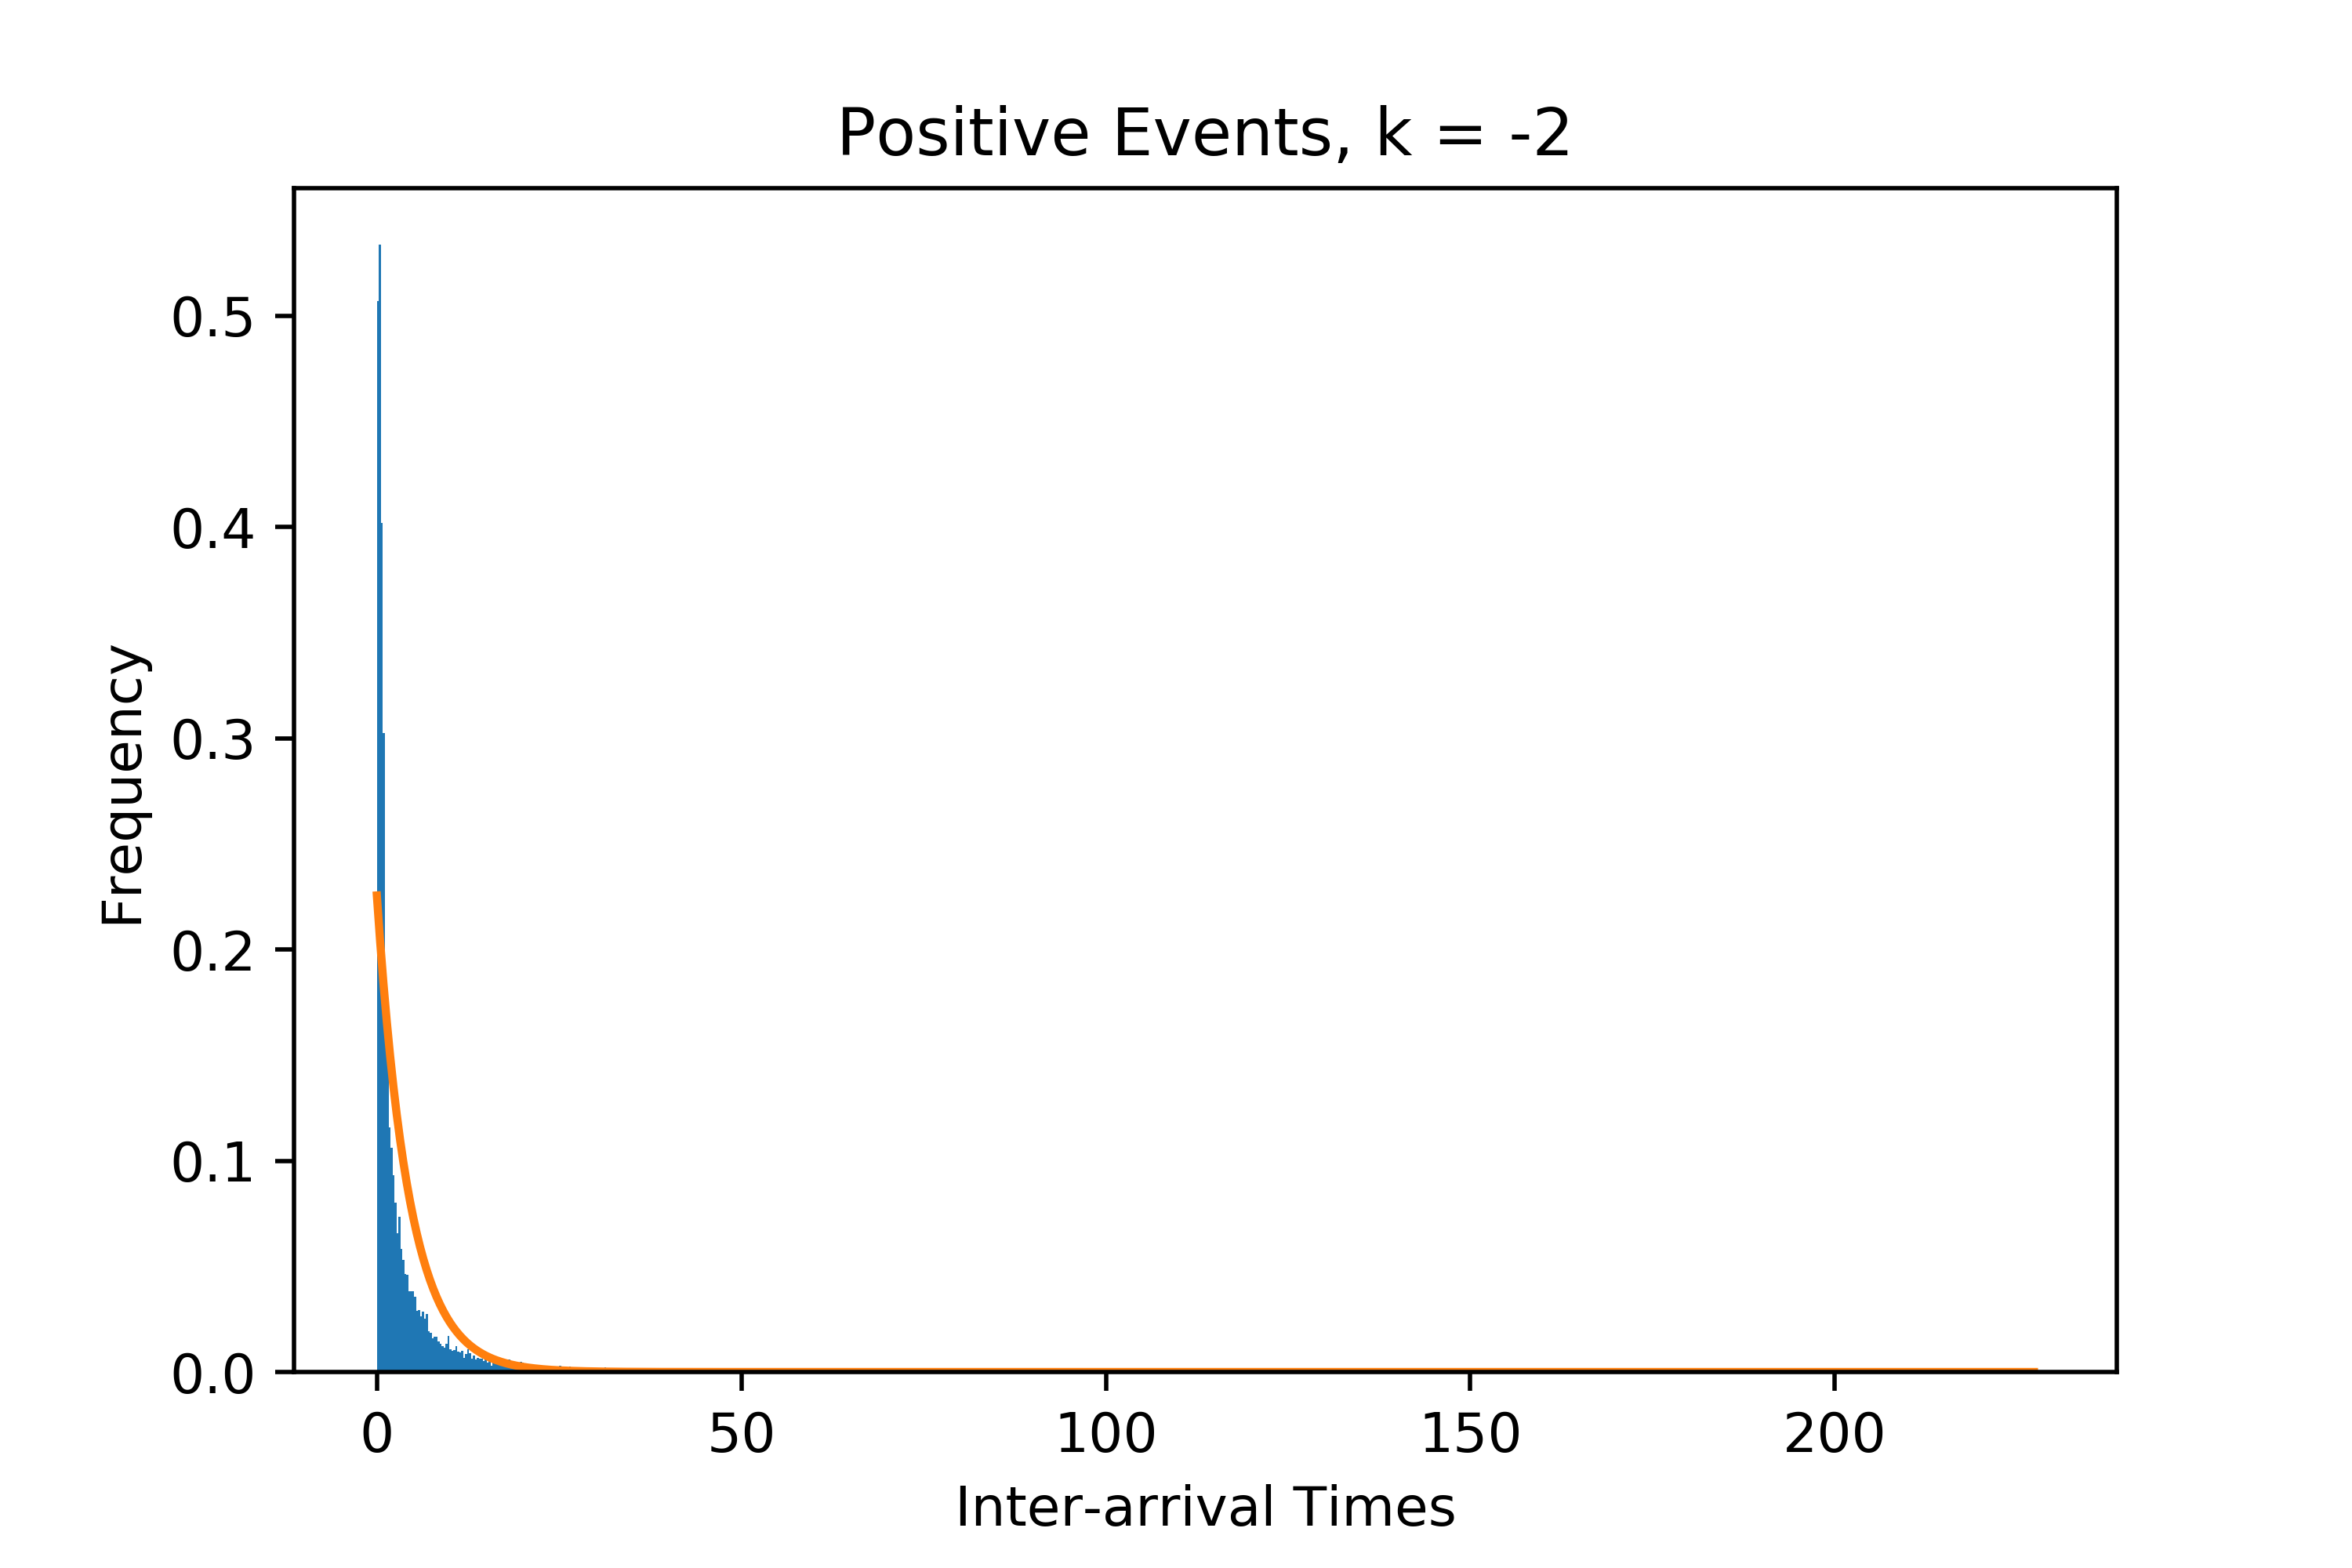
\includegraphics[width=60mm]{Figures/hist_pos_k-2.png}}
{}
\\
\subf{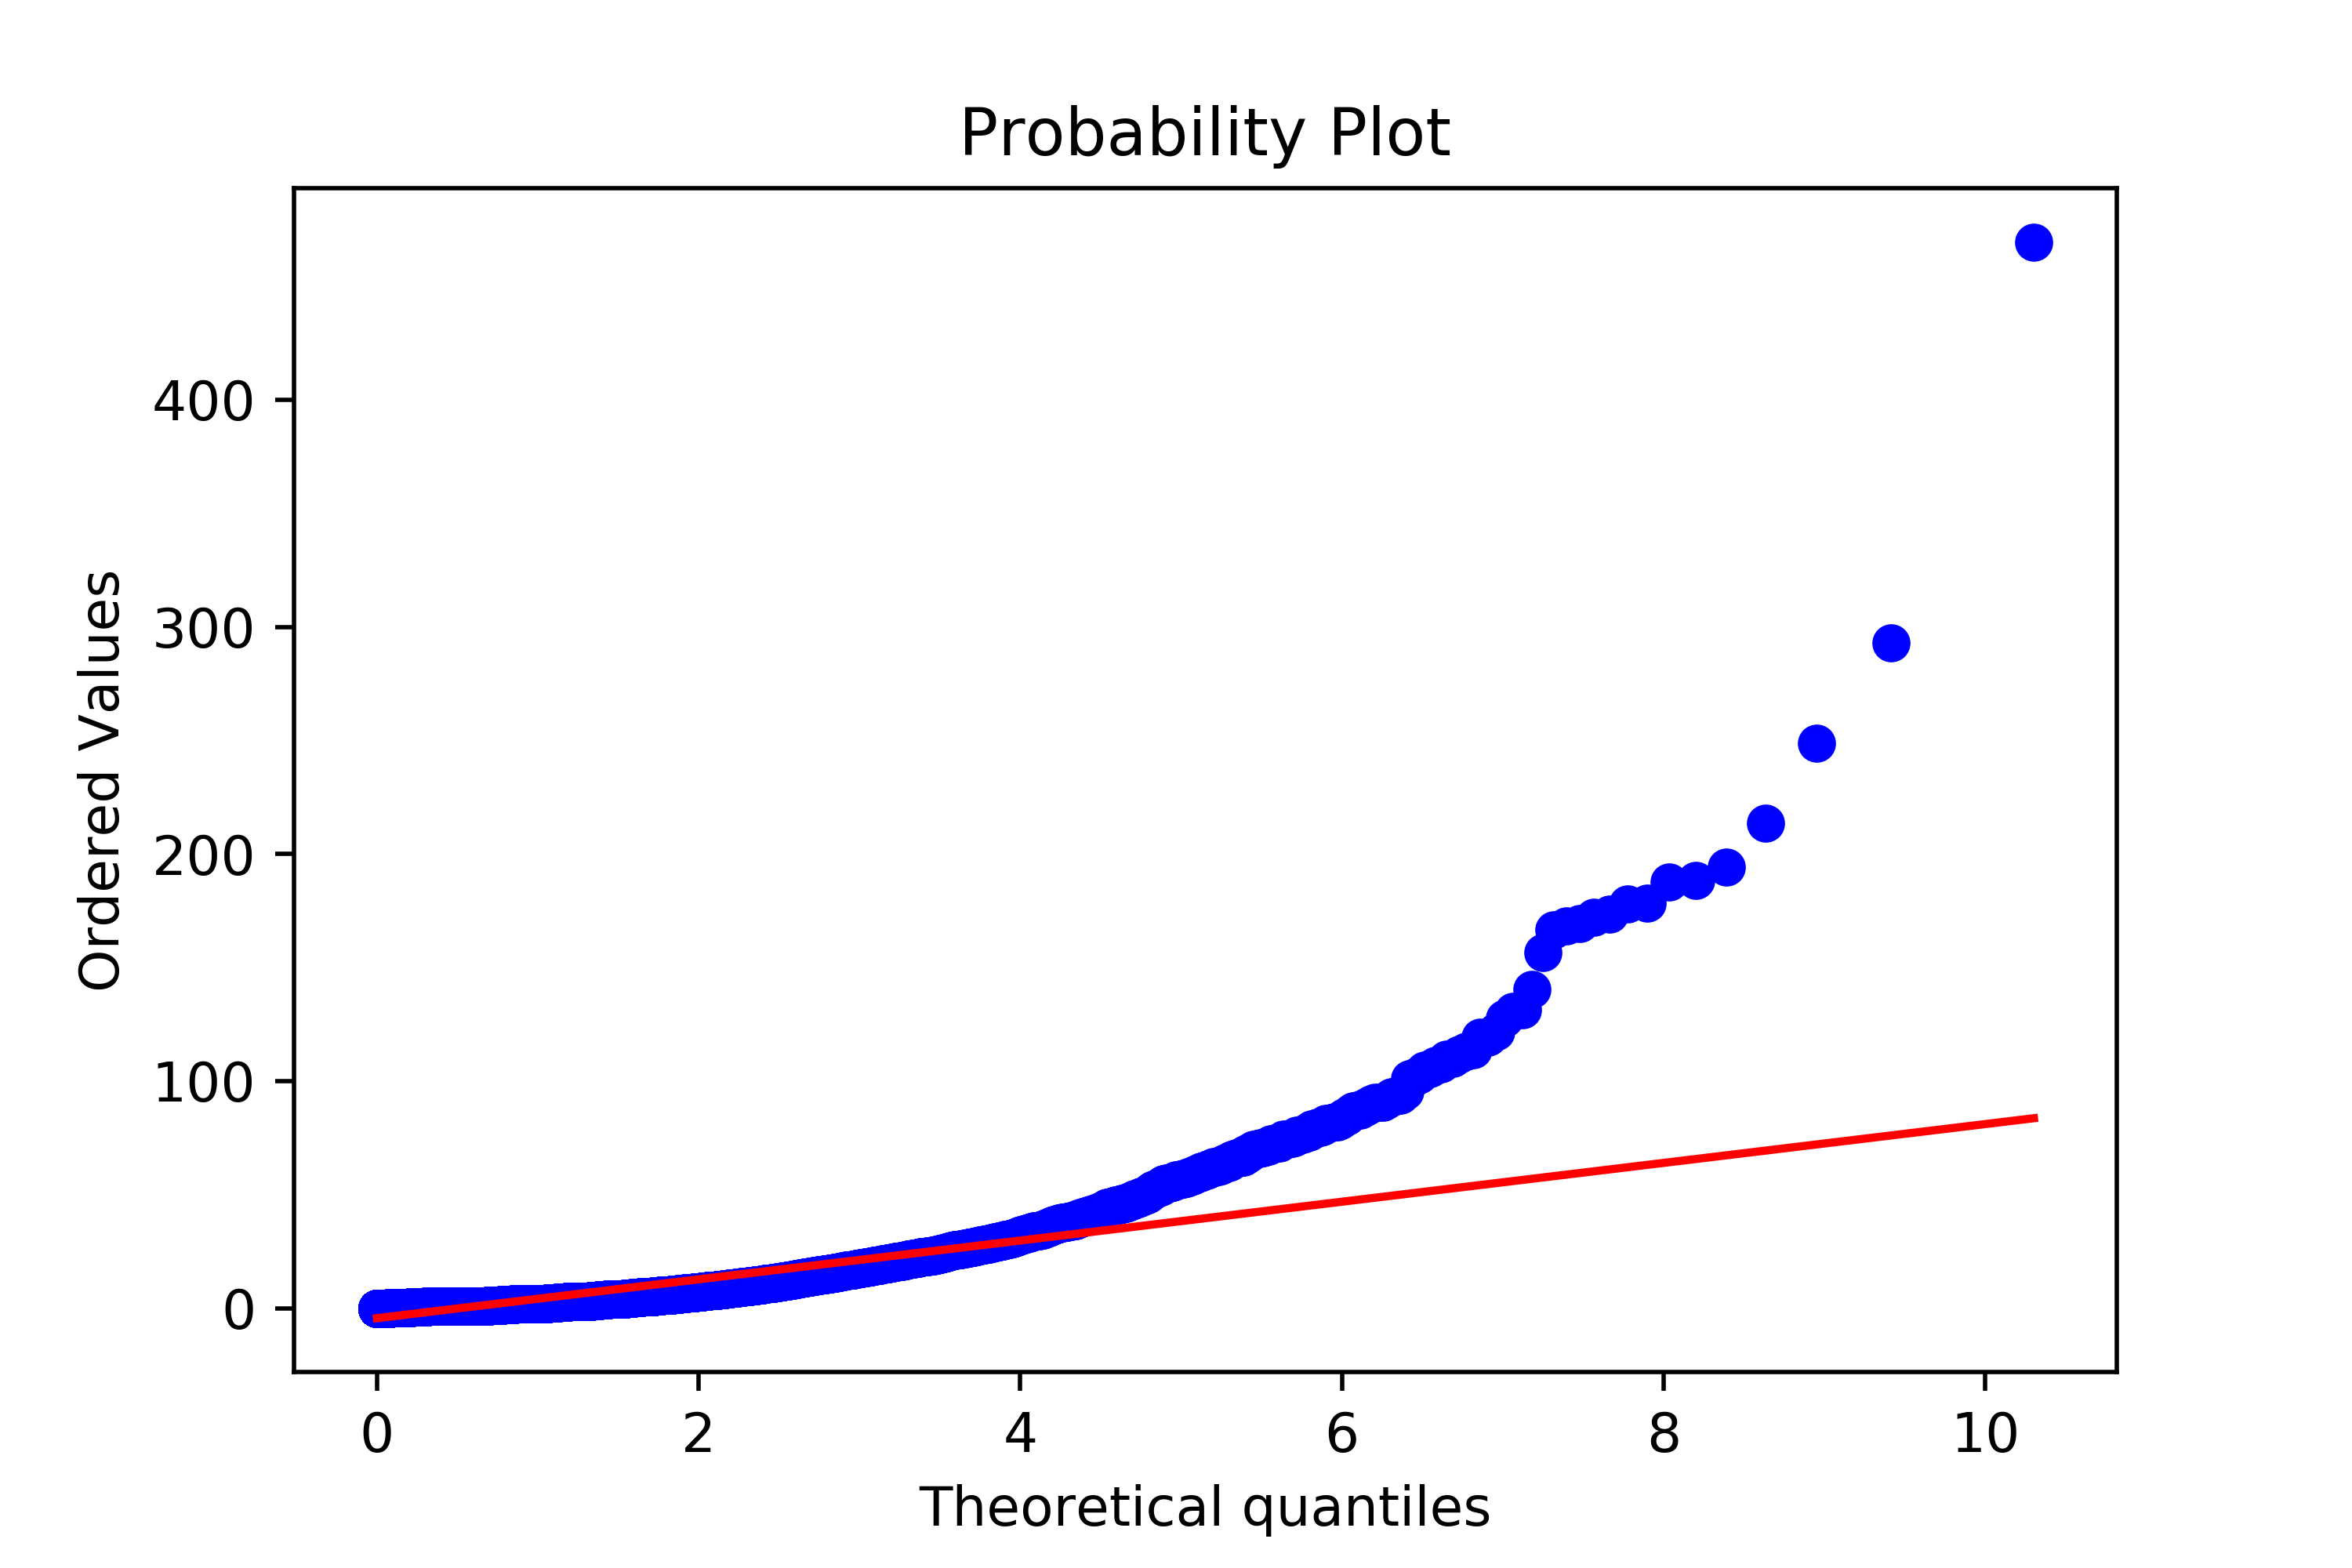
\includegraphics[width=60mm]{Figures/QQ_pos_k-1.png}}
{}
&
\subf{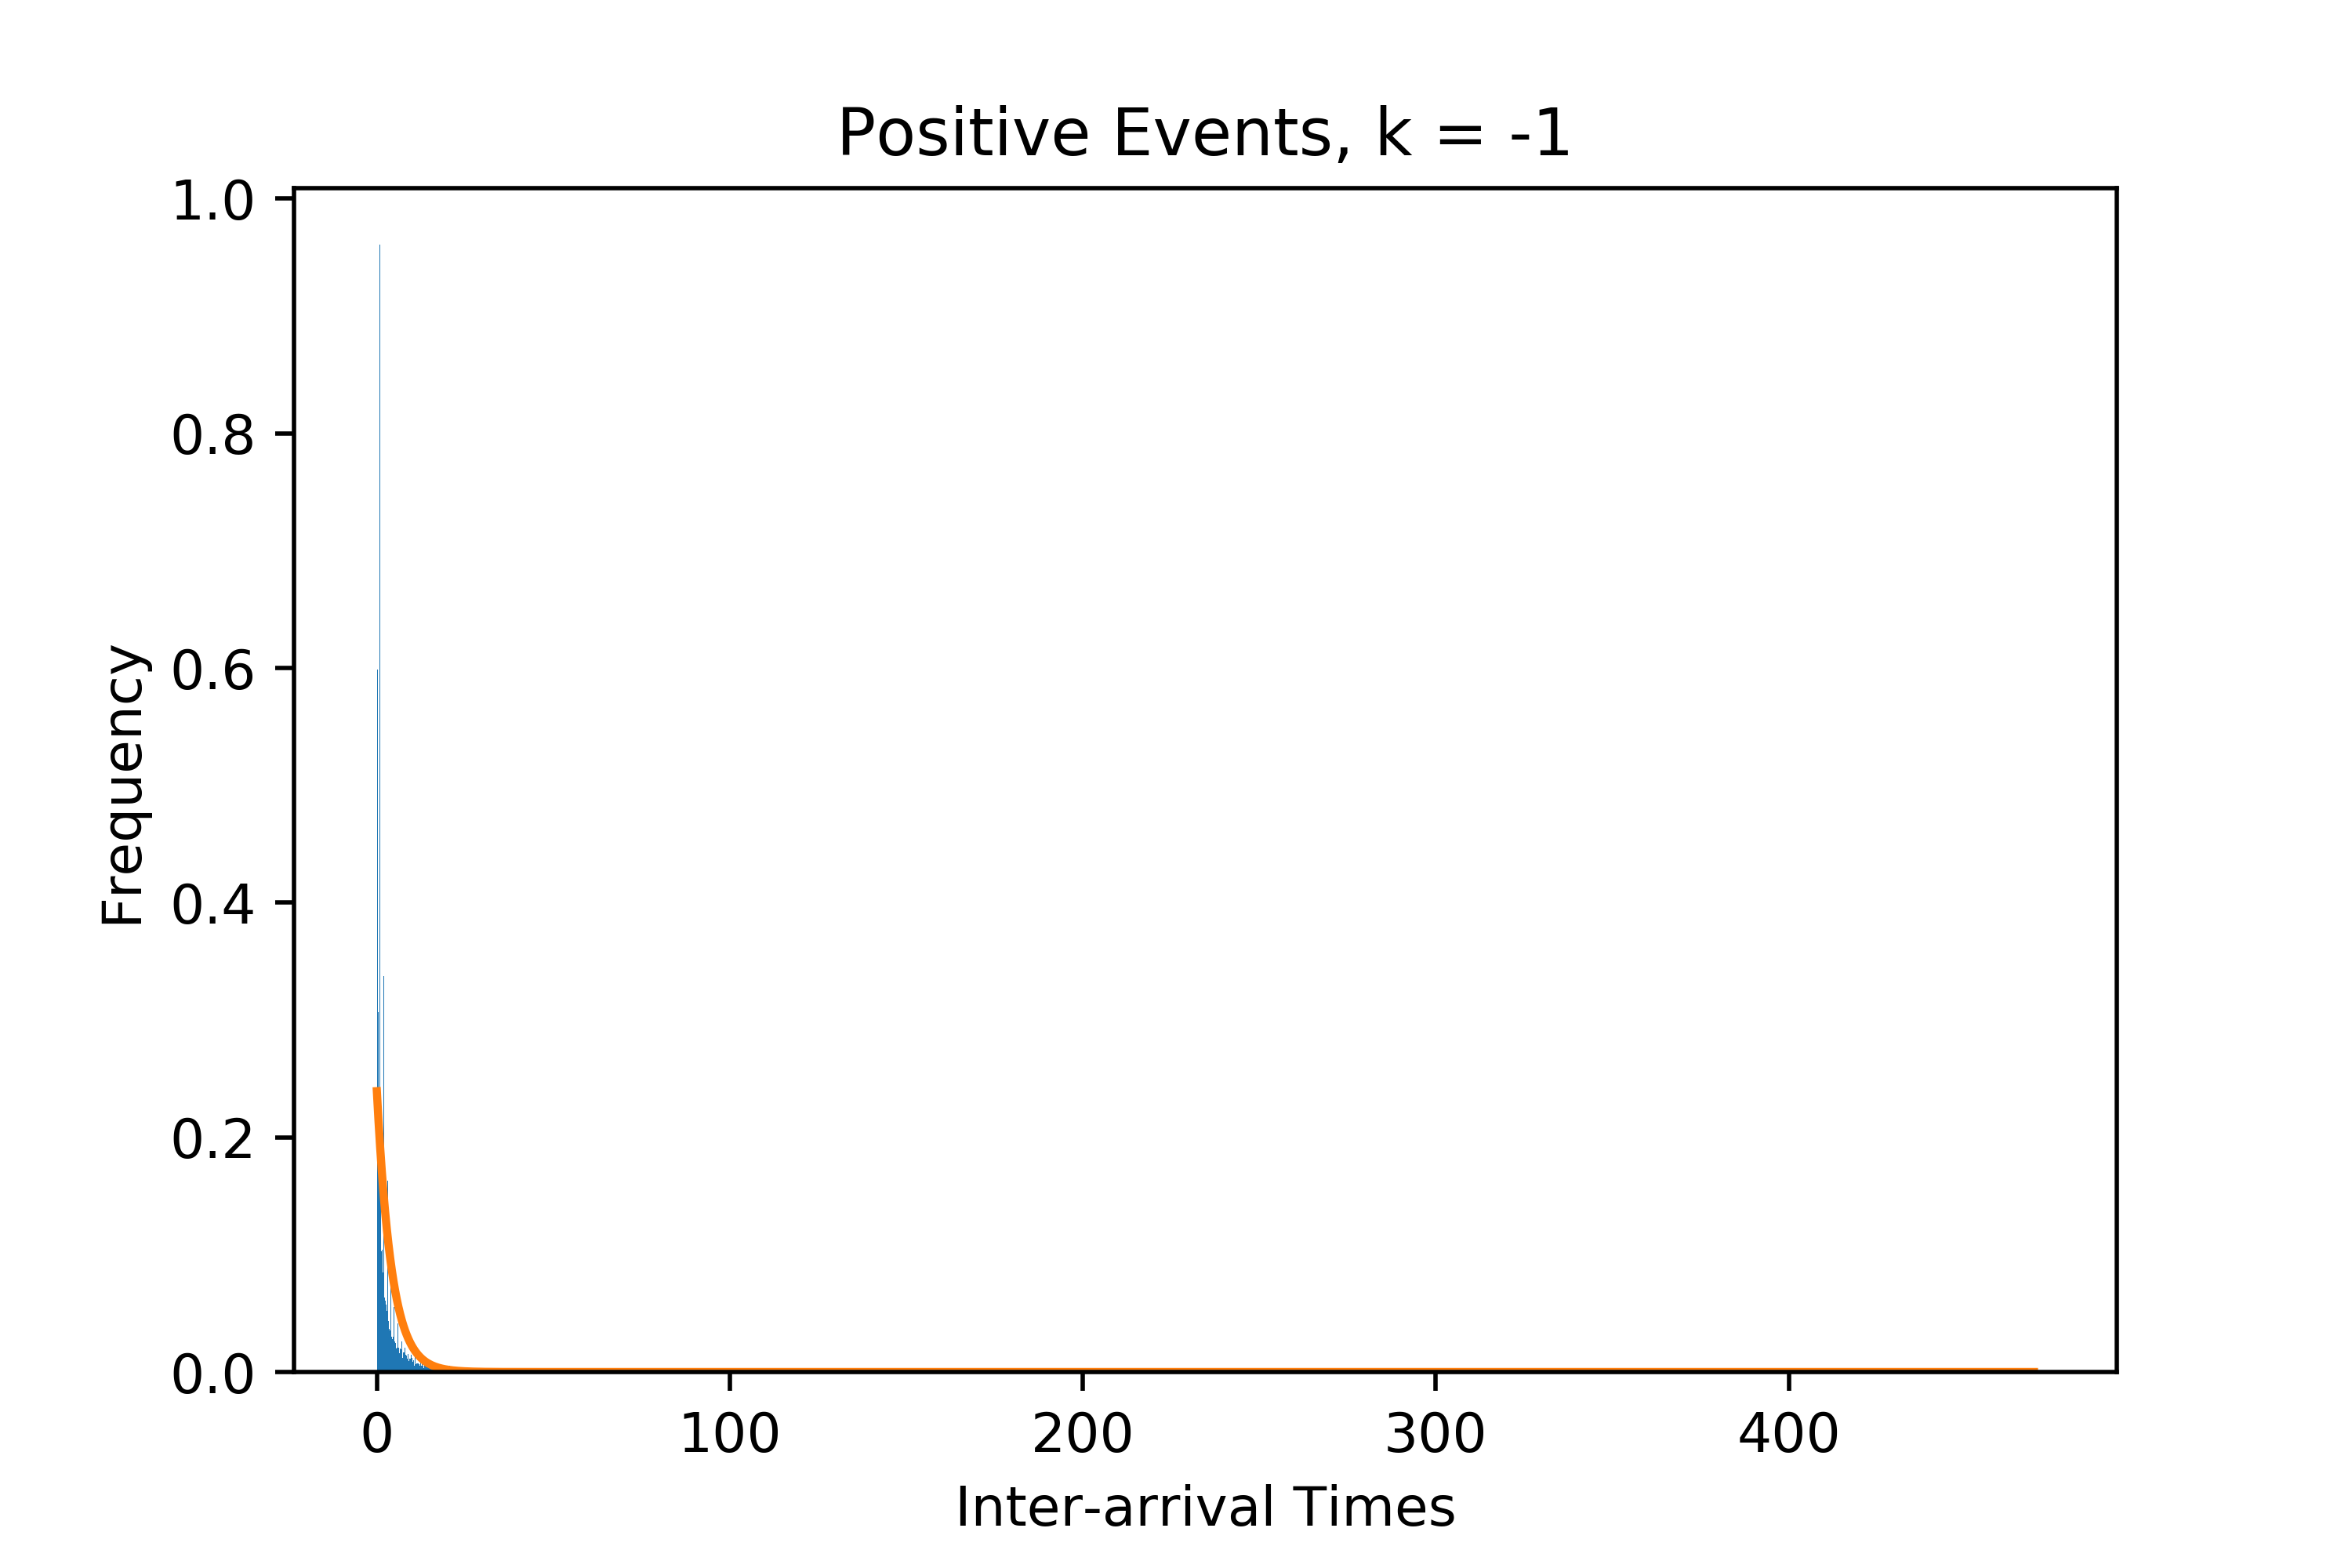
\includegraphics[width=60mm]{Figures/hist_pos_k-1.png}}
{}
\\
\subf{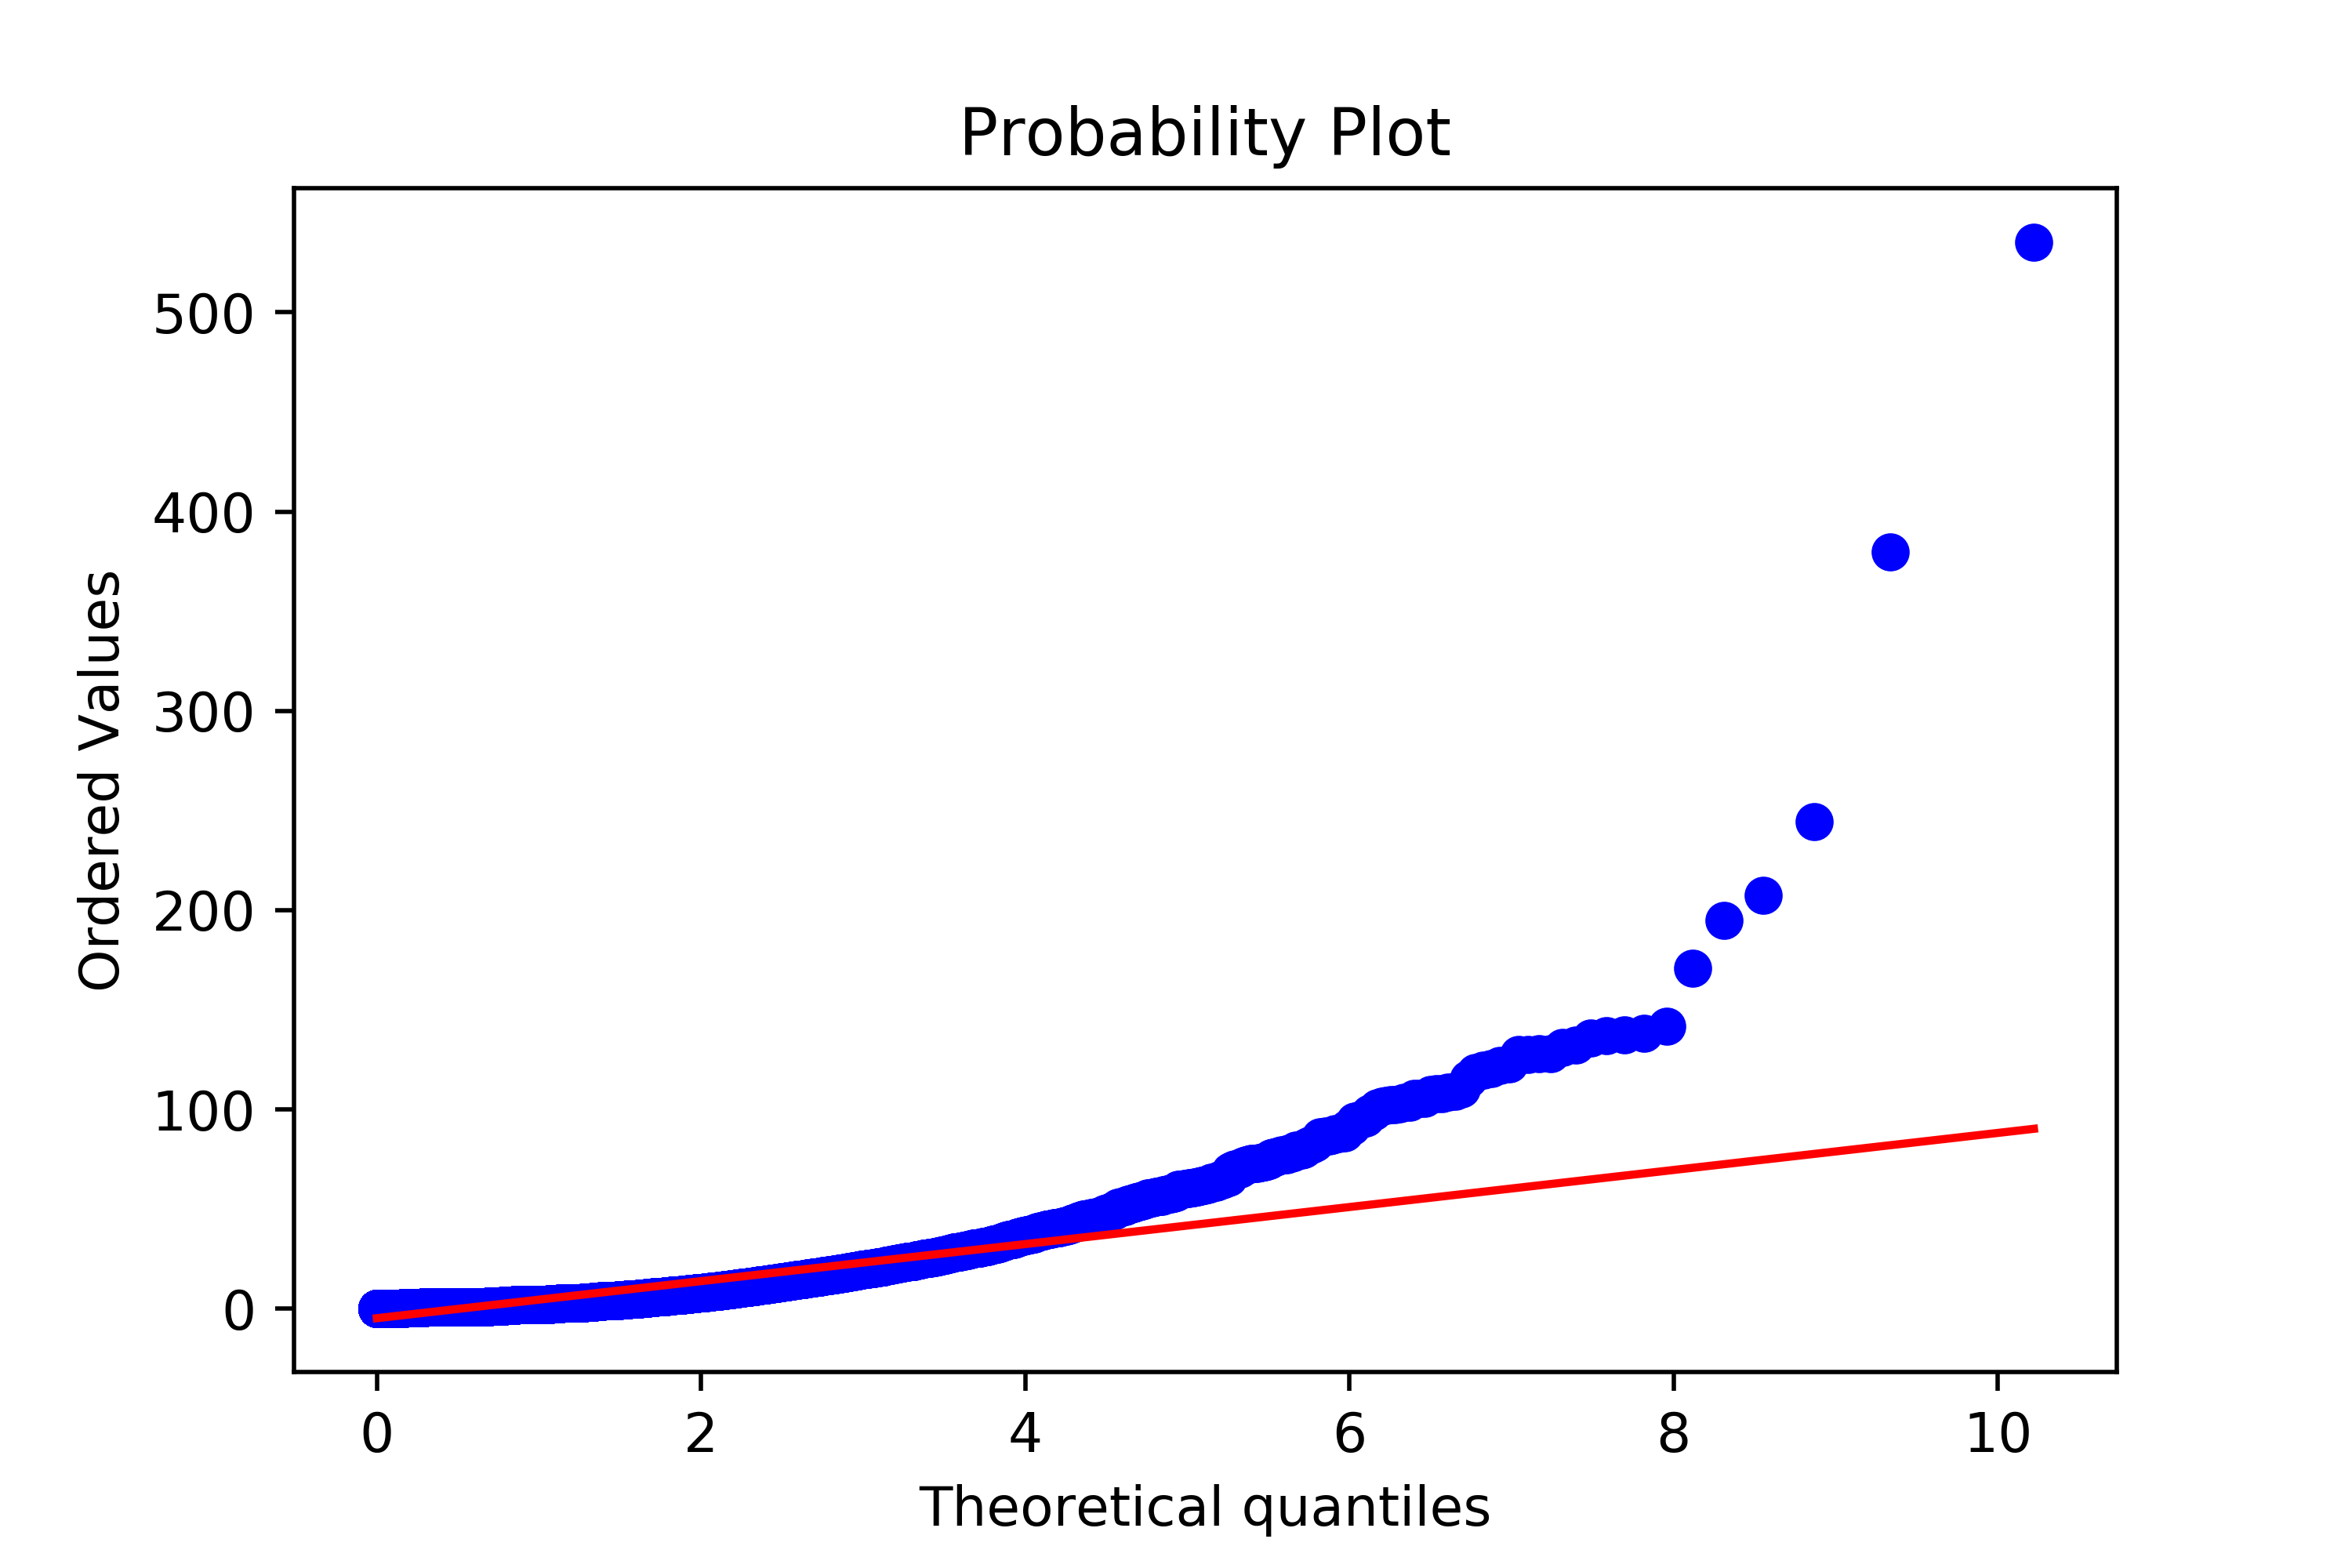
\includegraphics[width=60mm]{Figures/QQ_pos_k1.png}}
{}
&
\subf{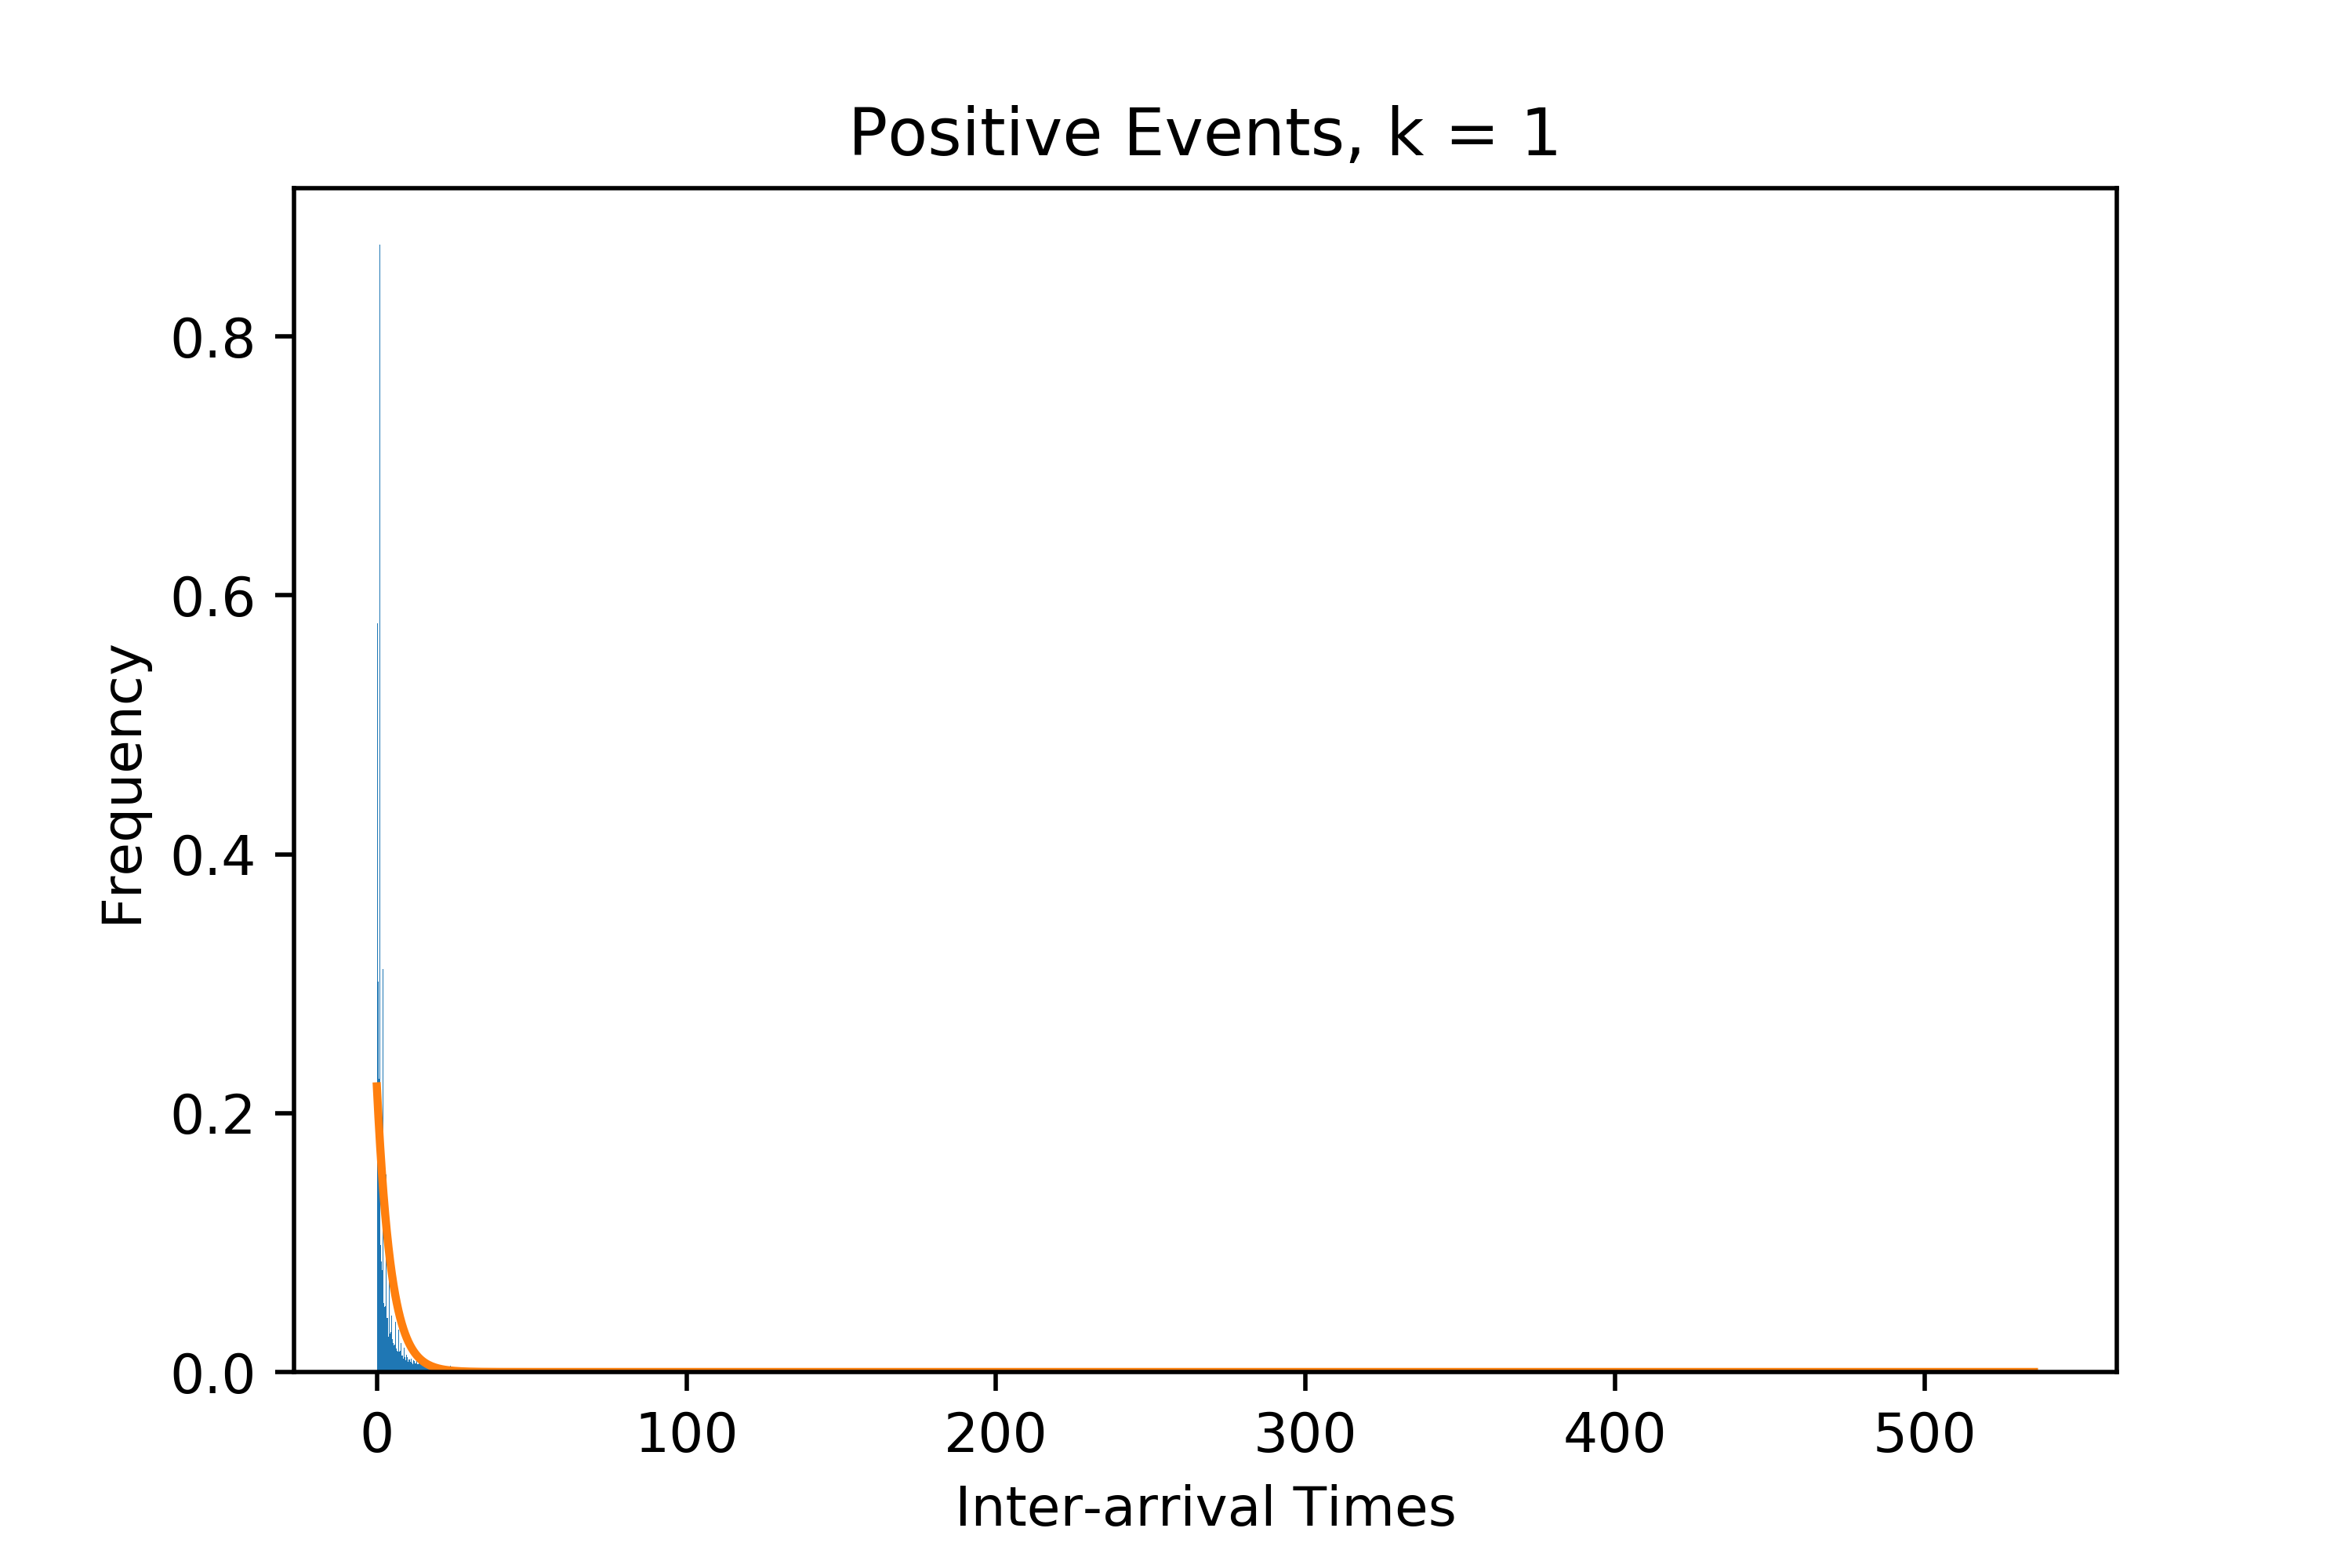
\includegraphics[width=60mm]{Figures/hist_pos_k1.png}}
{}
\\
\subf{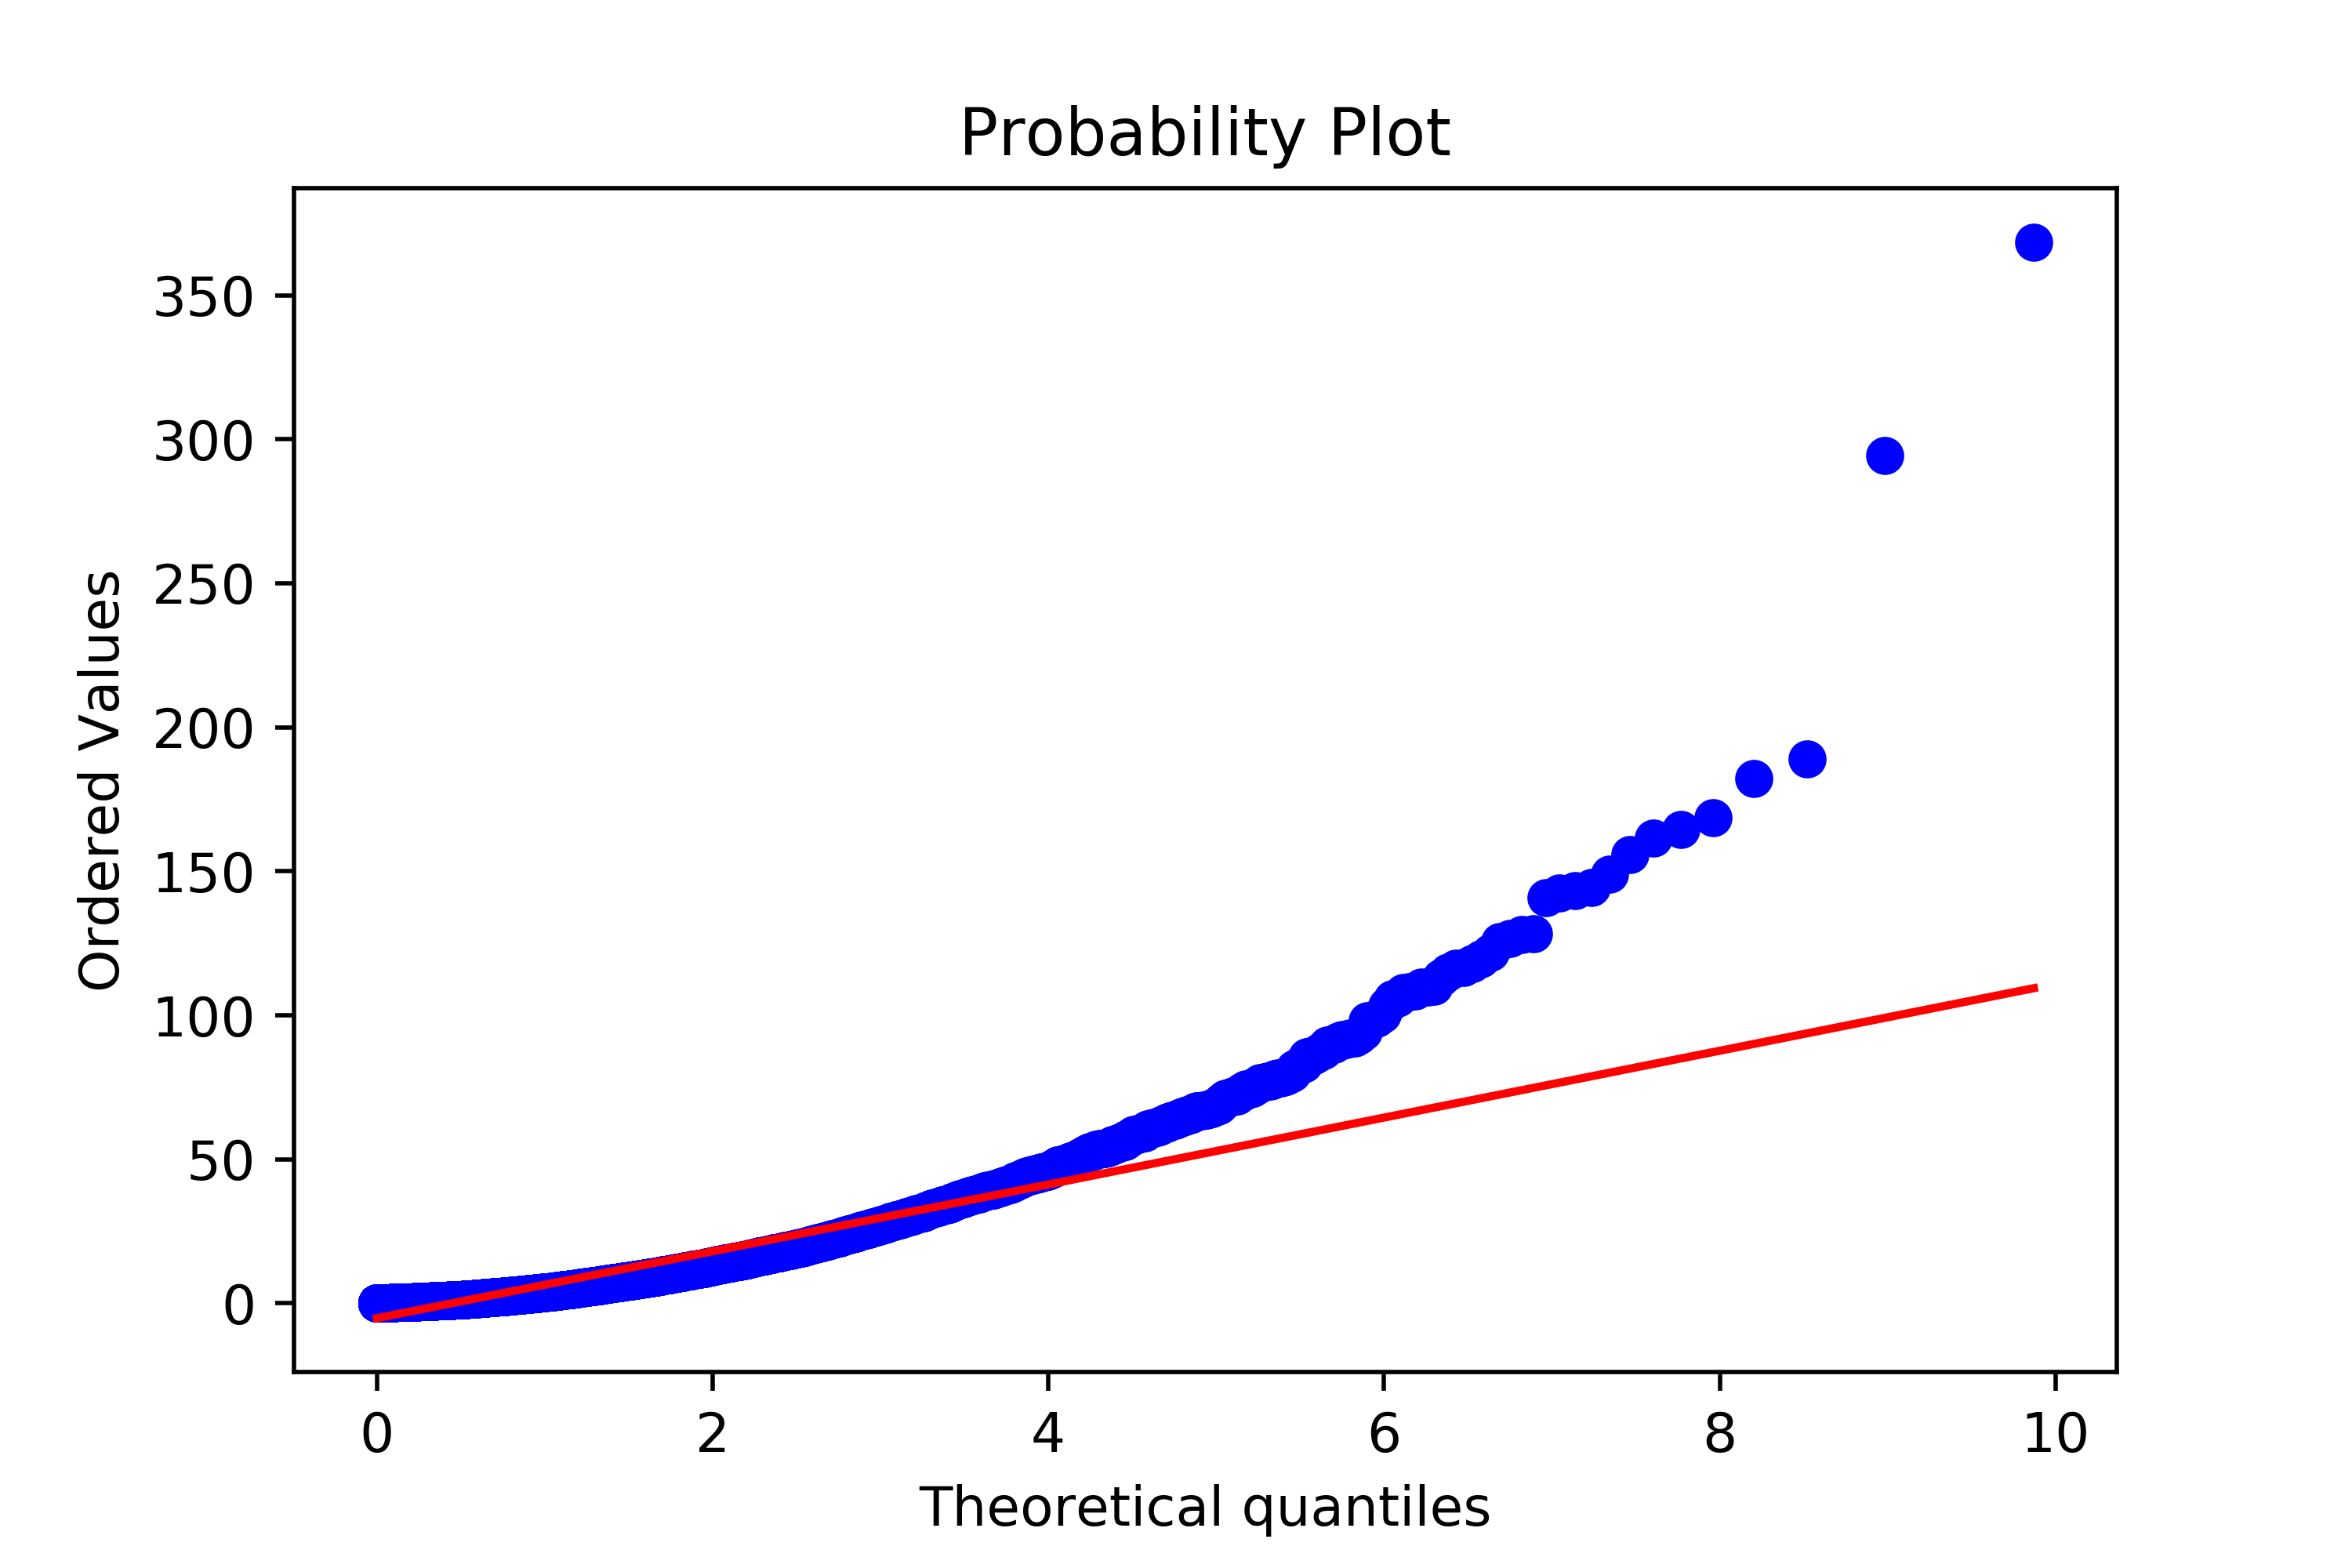
\includegraphics[width=60mm]{Figures/QQ_pos_k2.png}}
{}
&
\subf{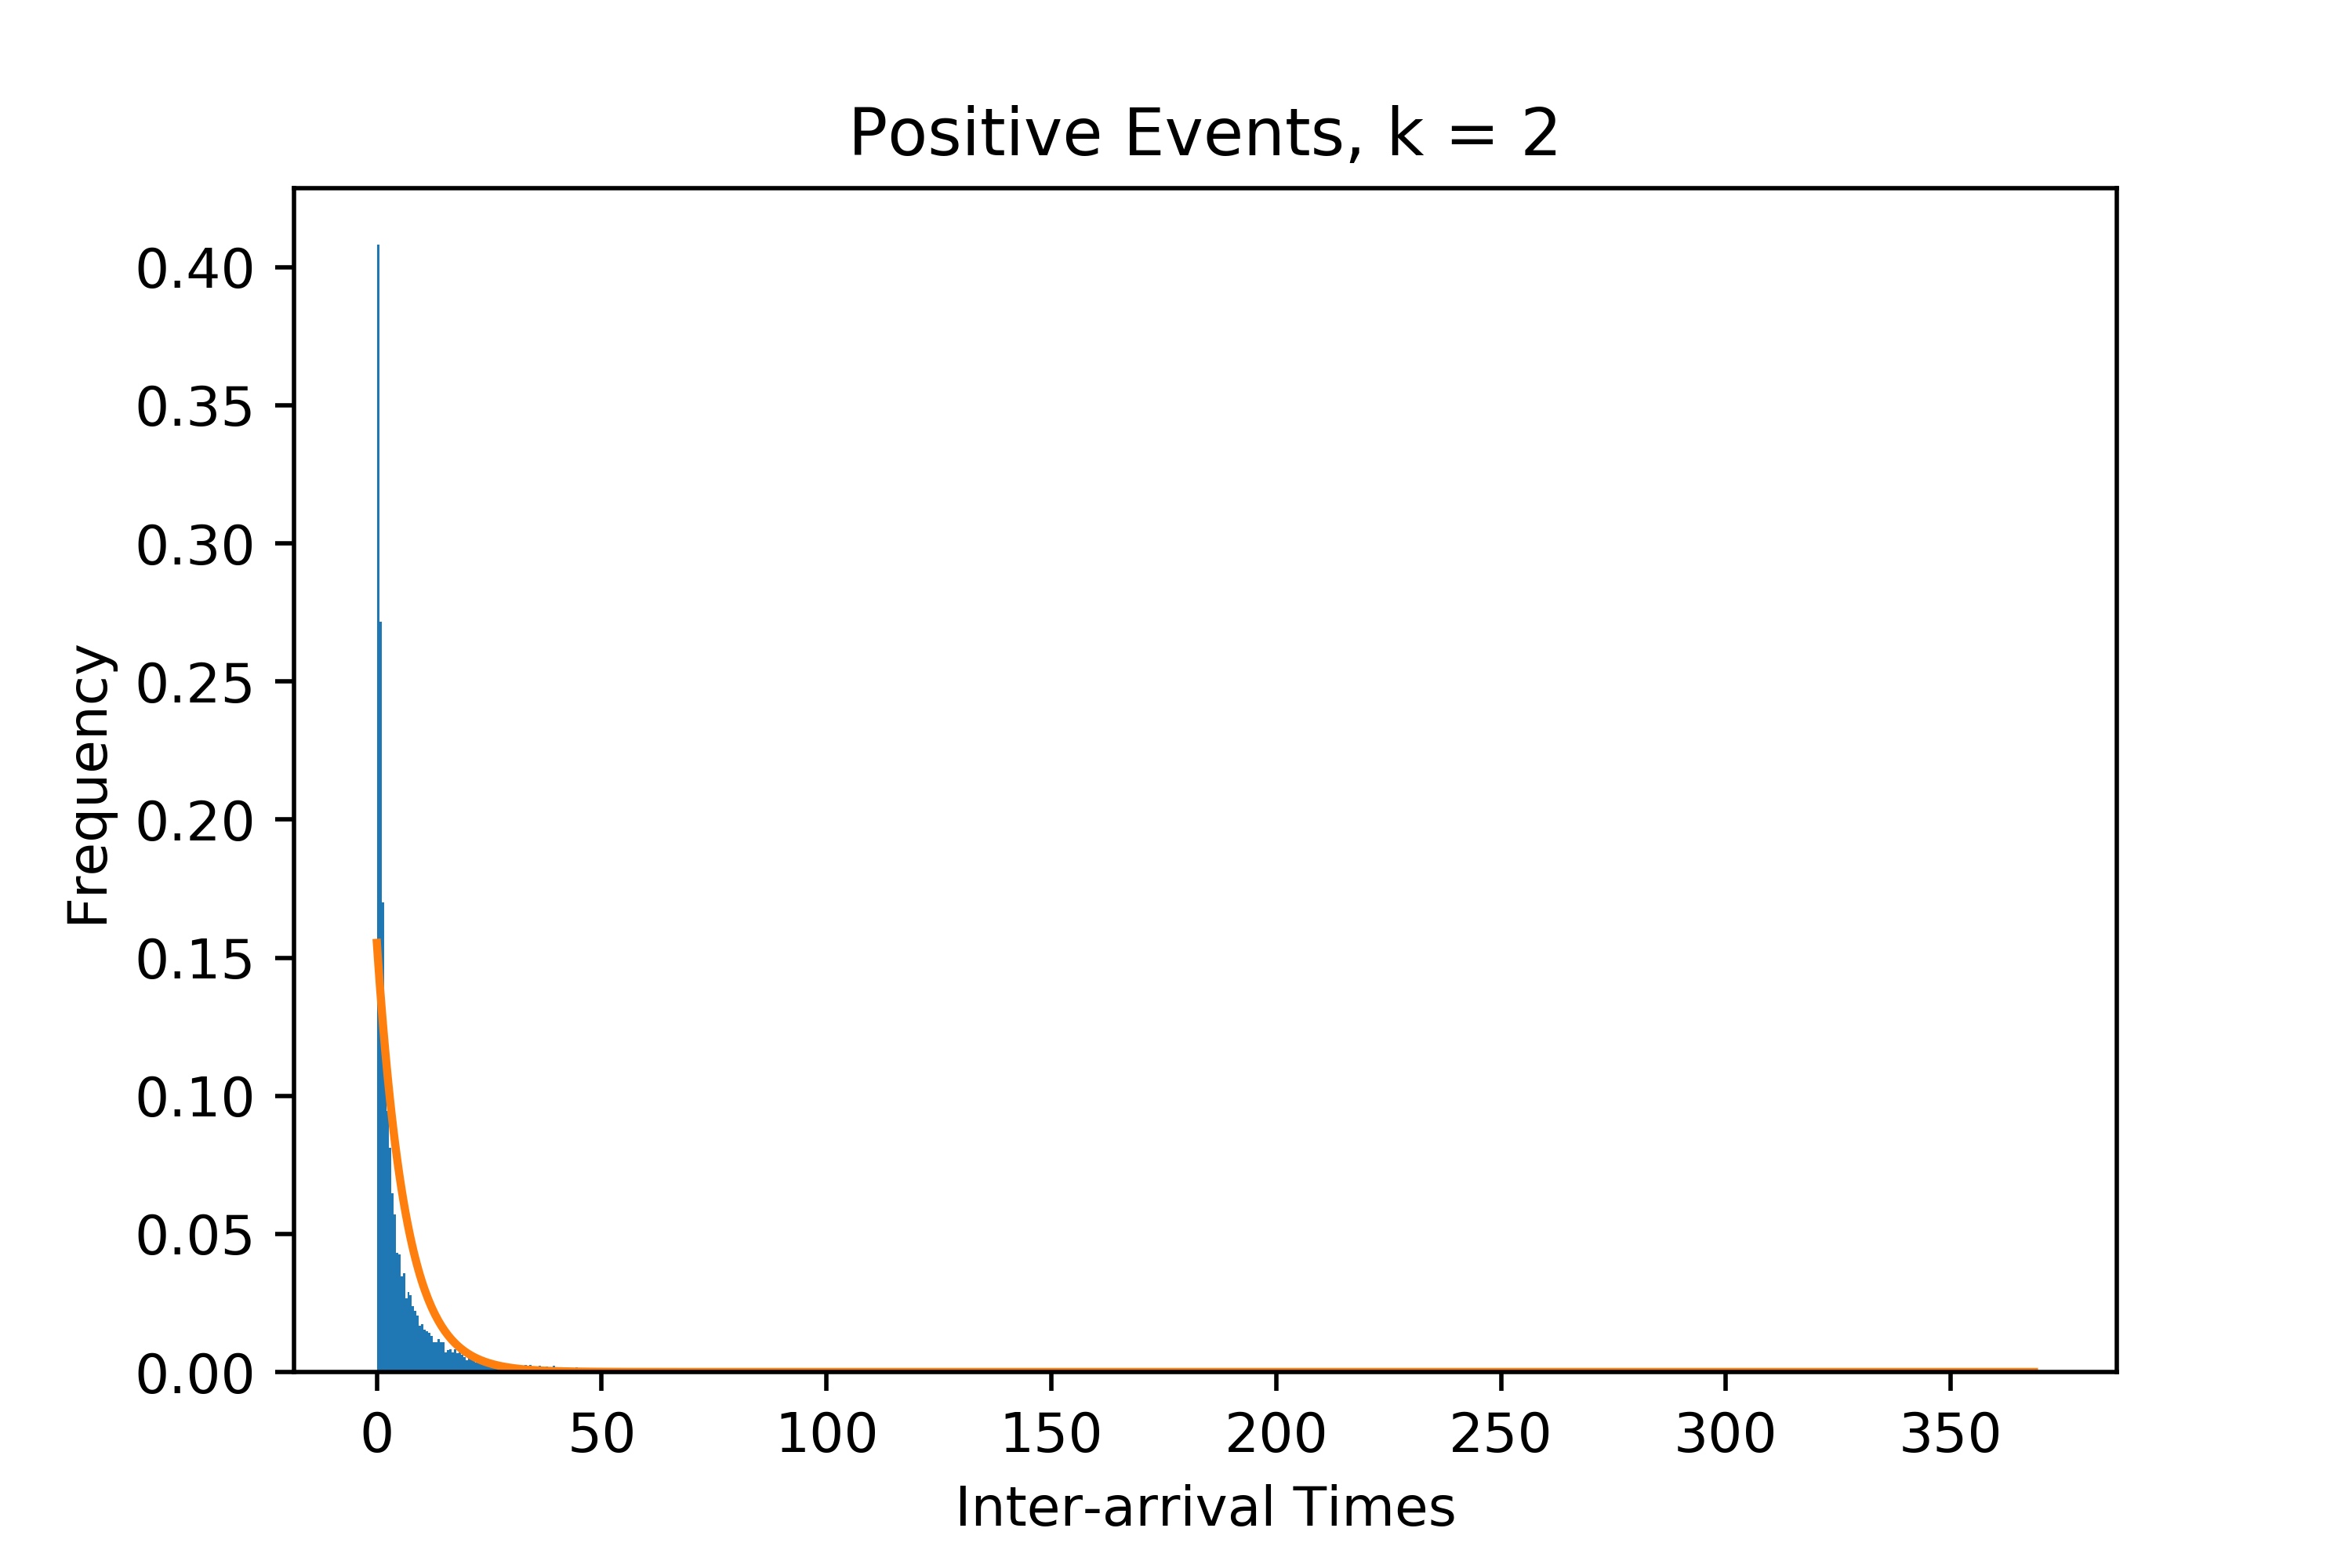
\includegraphics[width=60mm]{Figures/hist_pos_k2.png}}
{}
\\
\hline
\end{tabular}
\label{fig:interarrivals_pos}
\end{figure}

\begin{figure}
\centering
\caption{Inter-Arrival Times for Negative Events Compared to Exponential Distribution (4 Positions Closest to $p_0$)}
\begin{tabular}{cc}
\hline
\subf{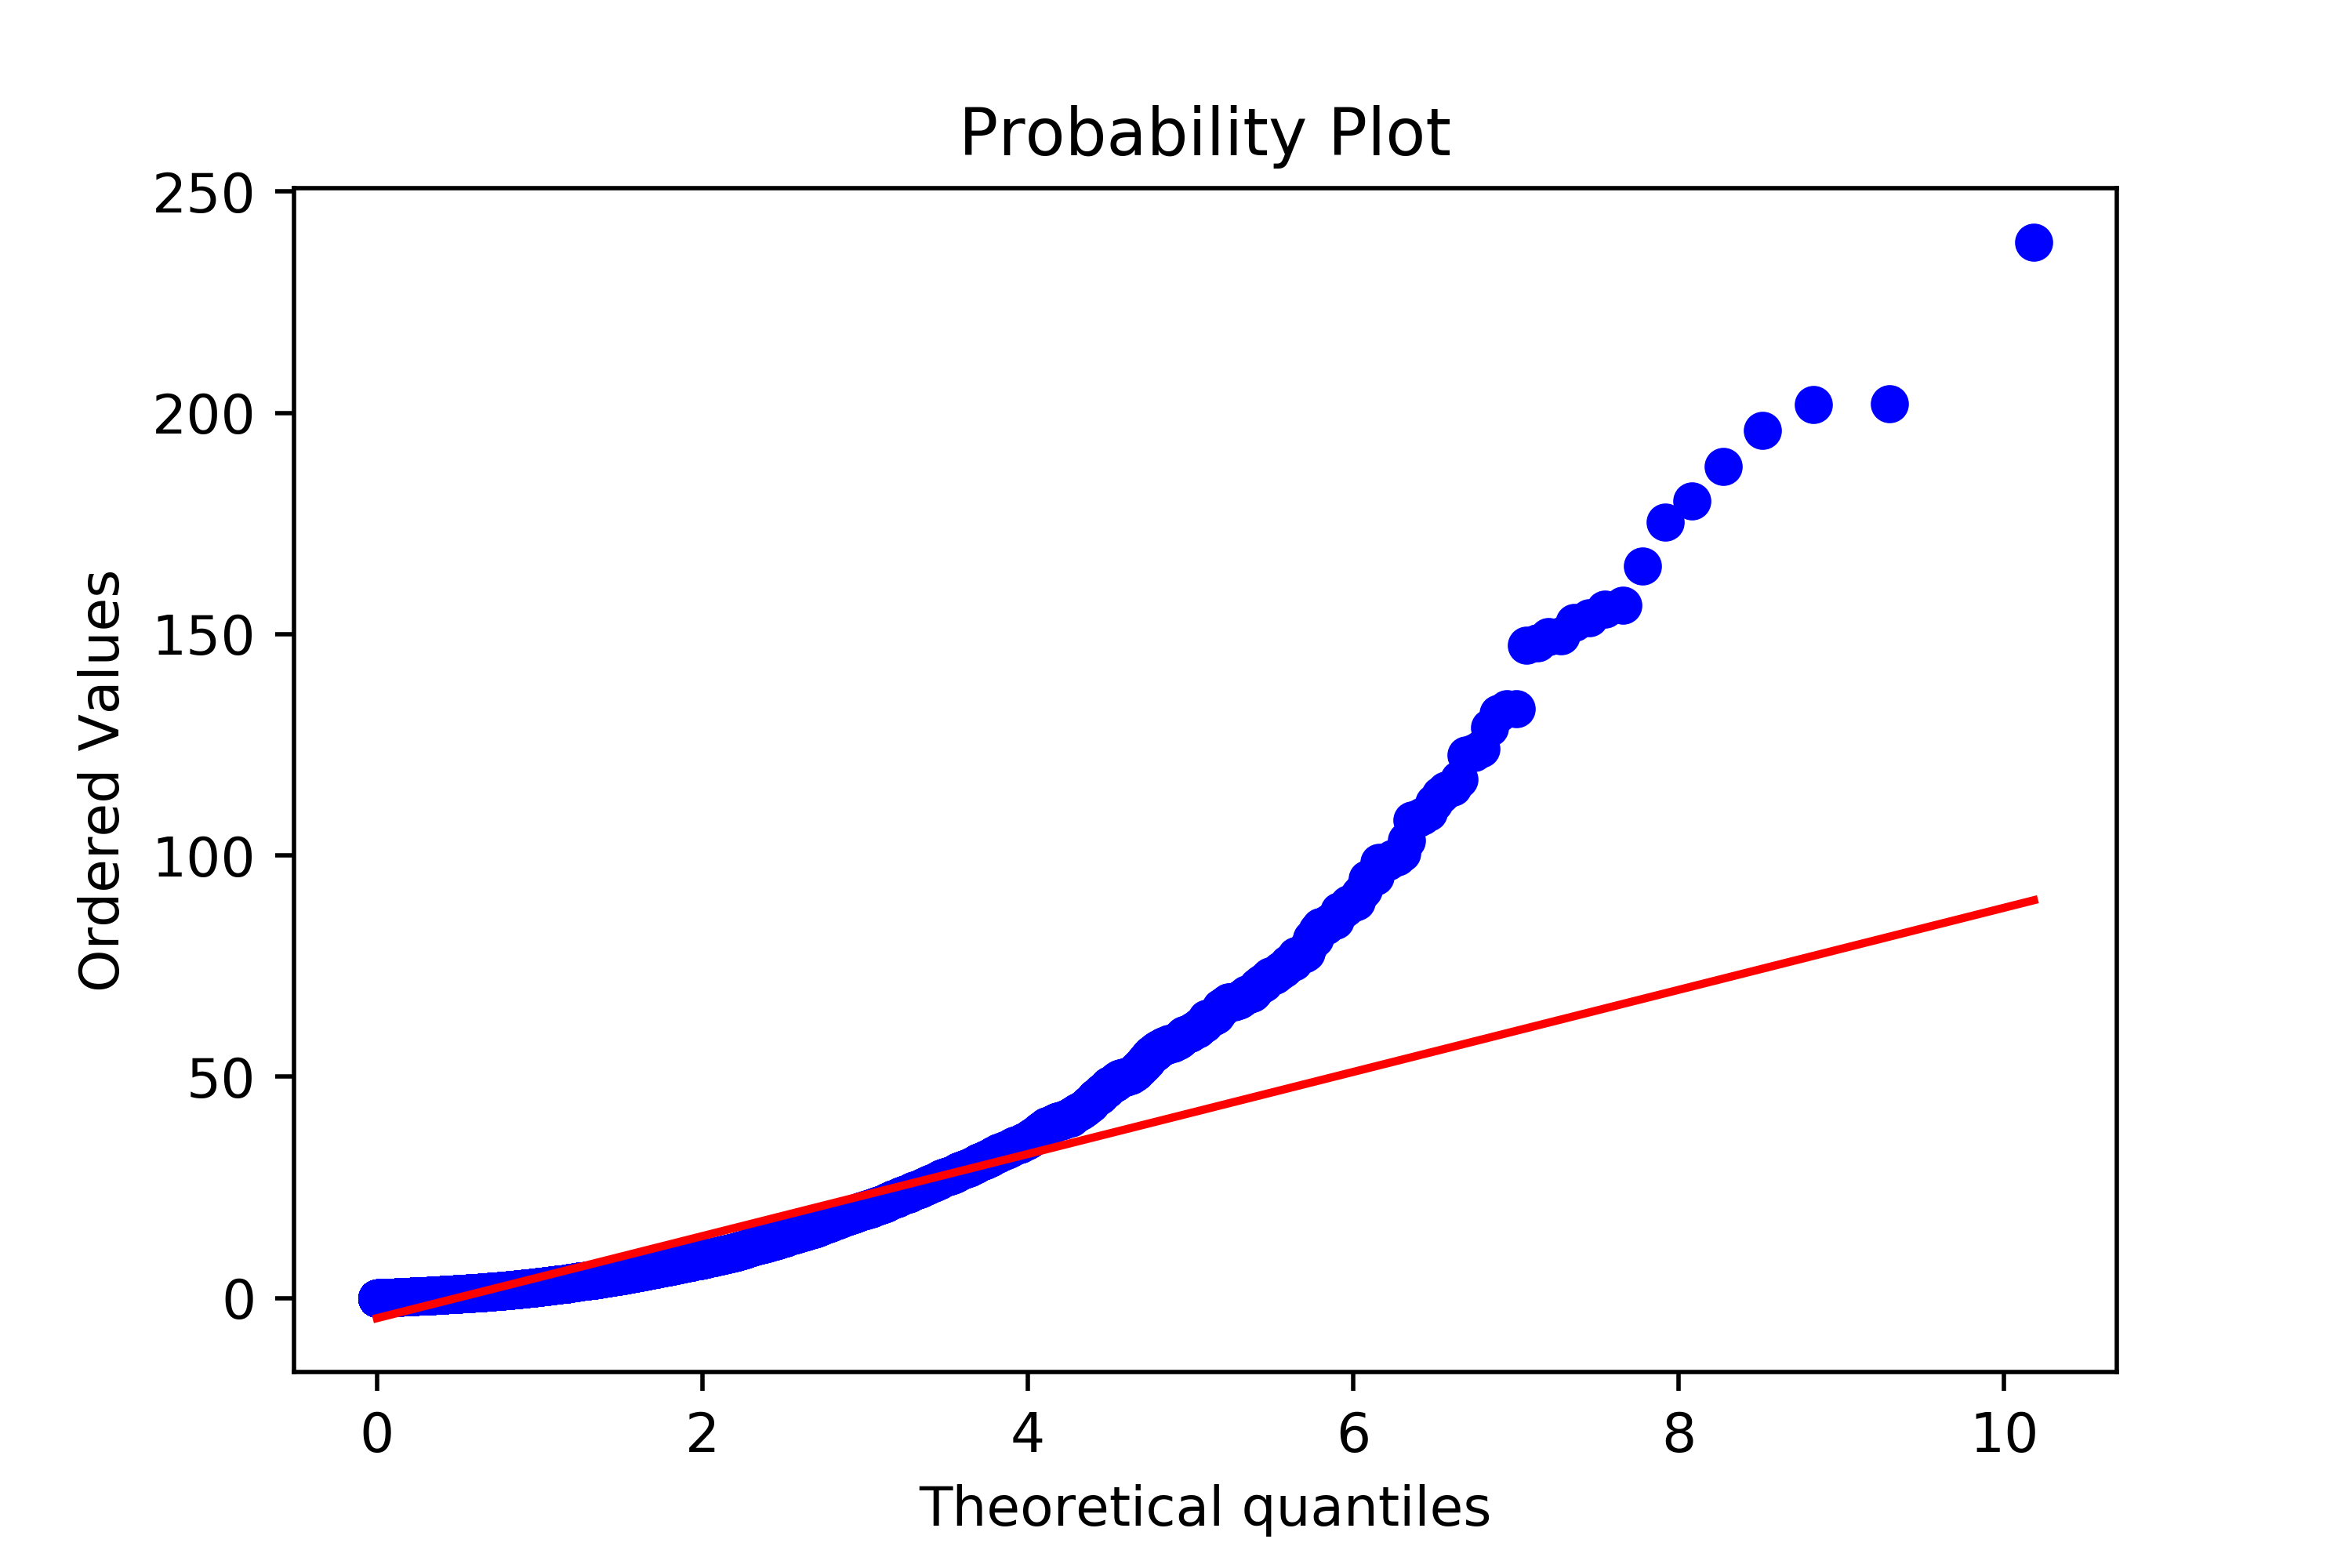
\includegraphics[width=60mm]{Figures/QQ_neg_k-2.png}}
{}
&
\subf{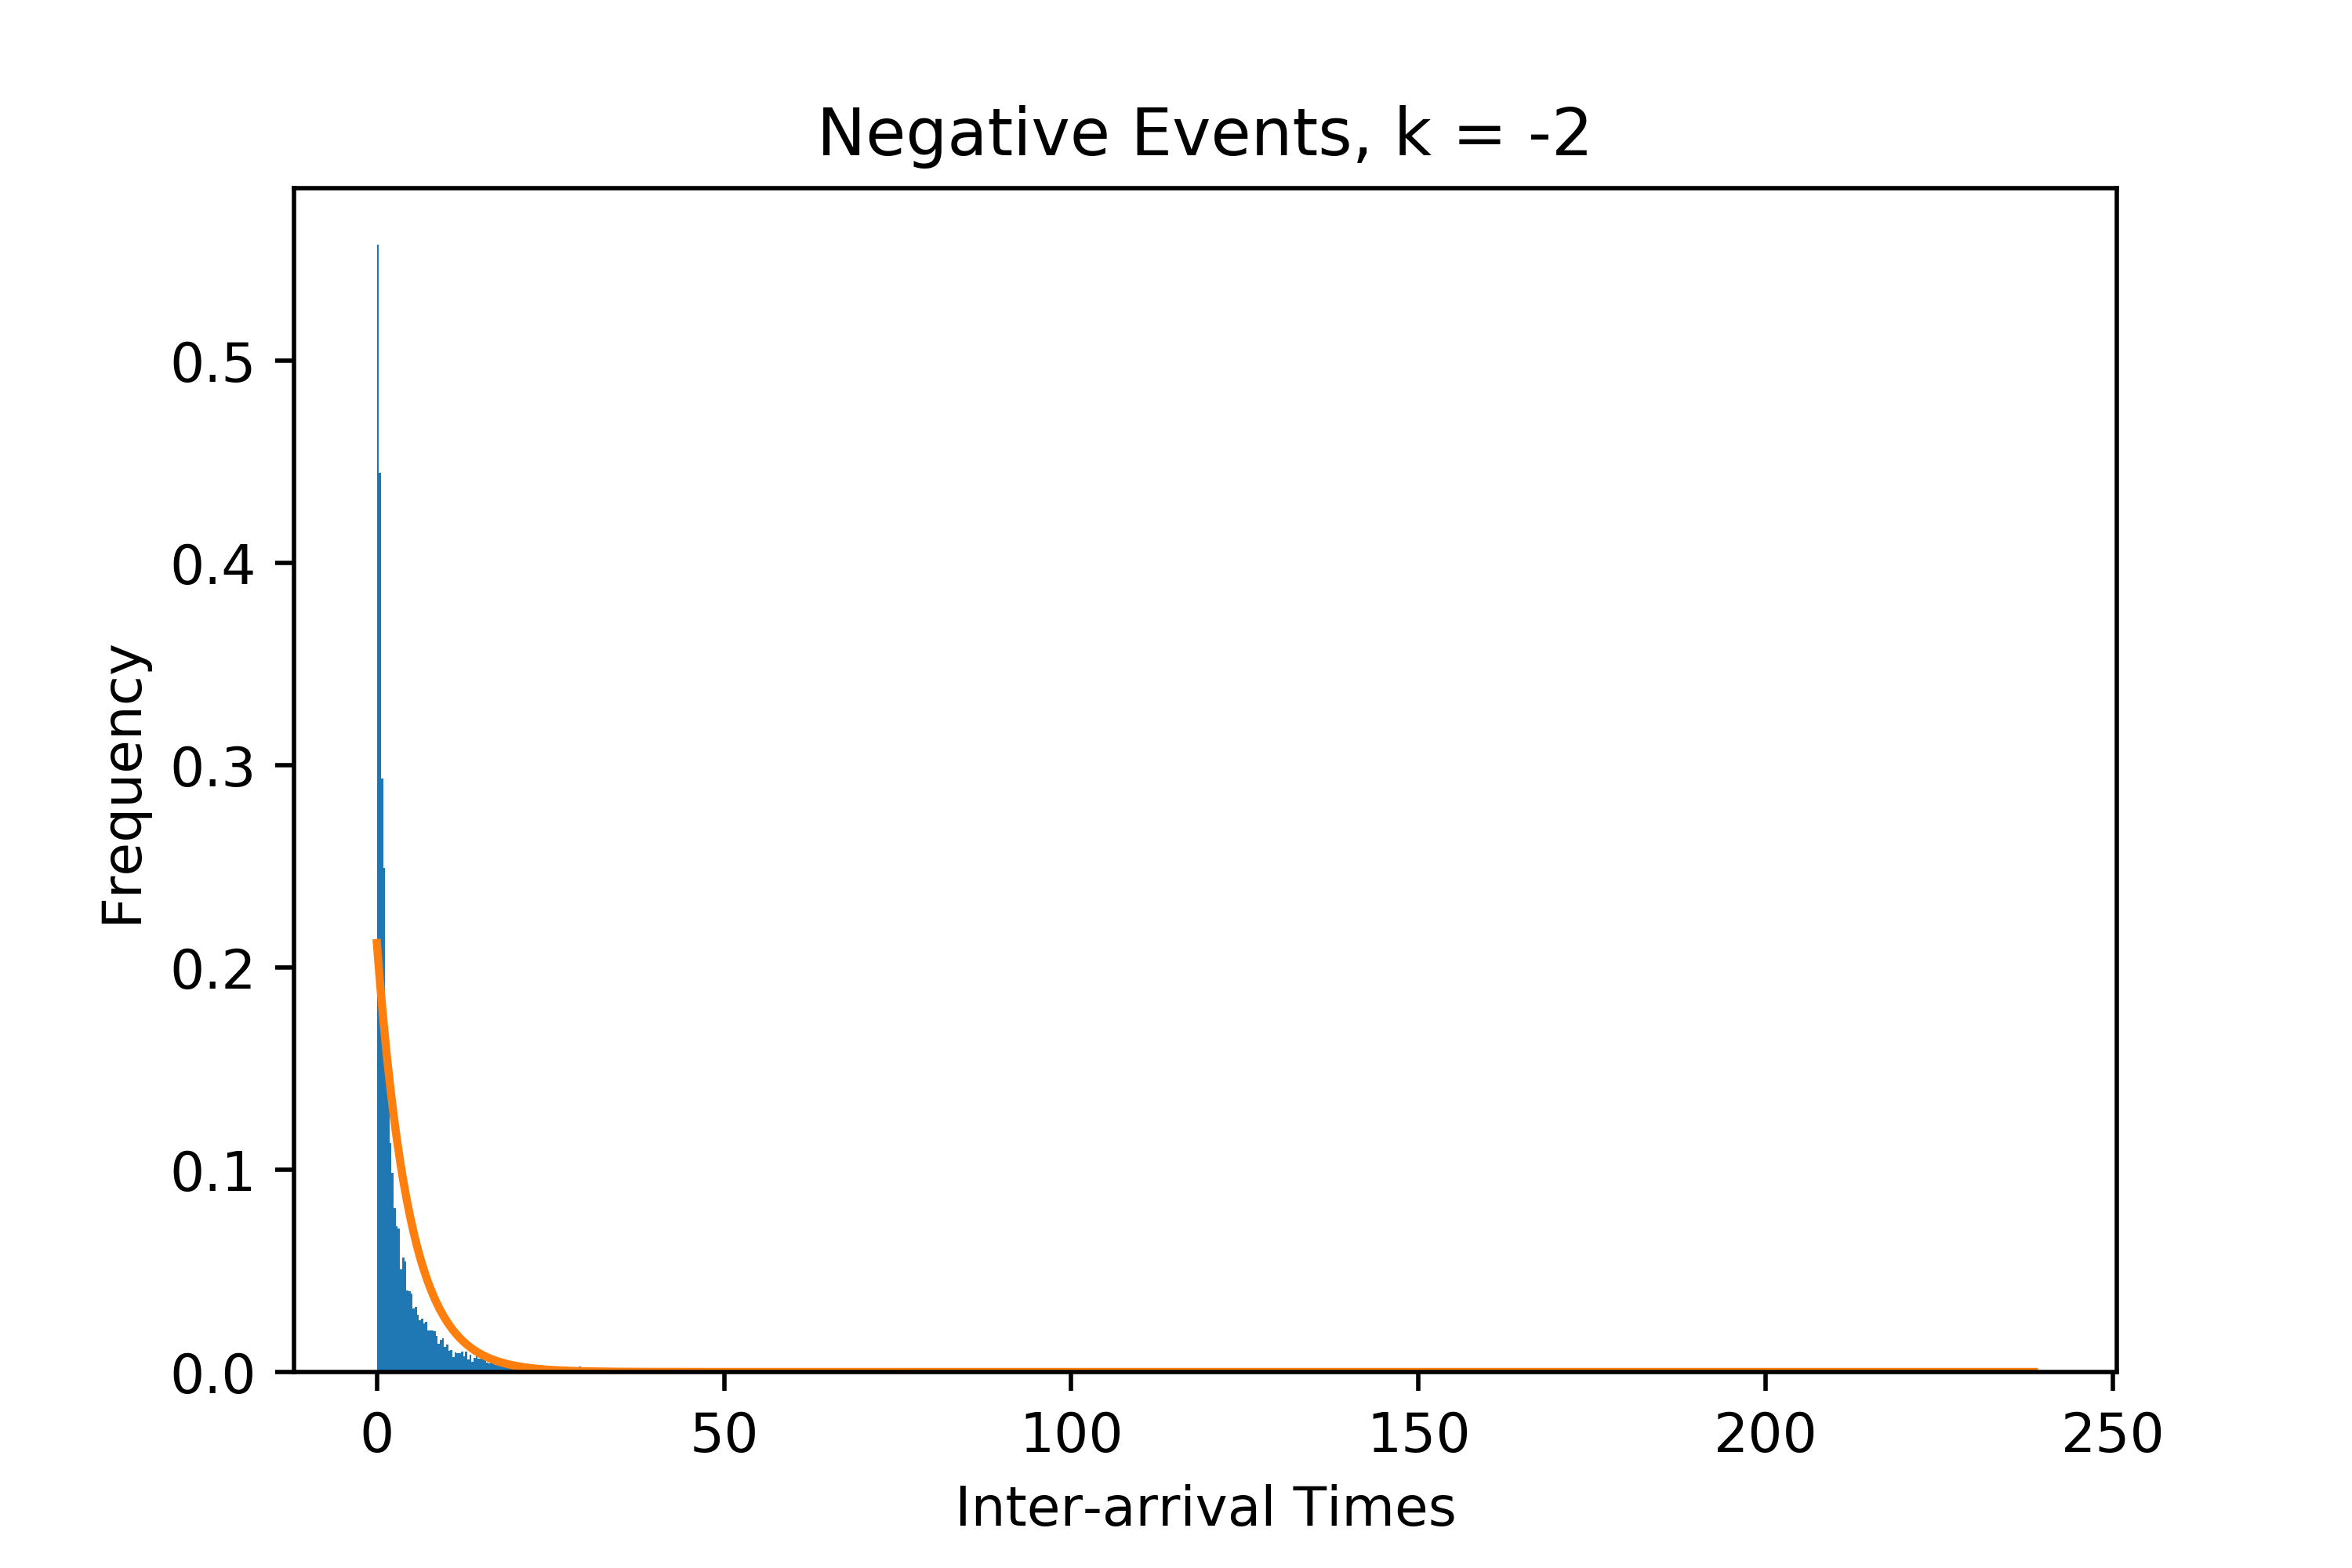
\includegraphics[width=60mm]{Figures/hist_neg_k-2.png}}
{}
\\
\subf{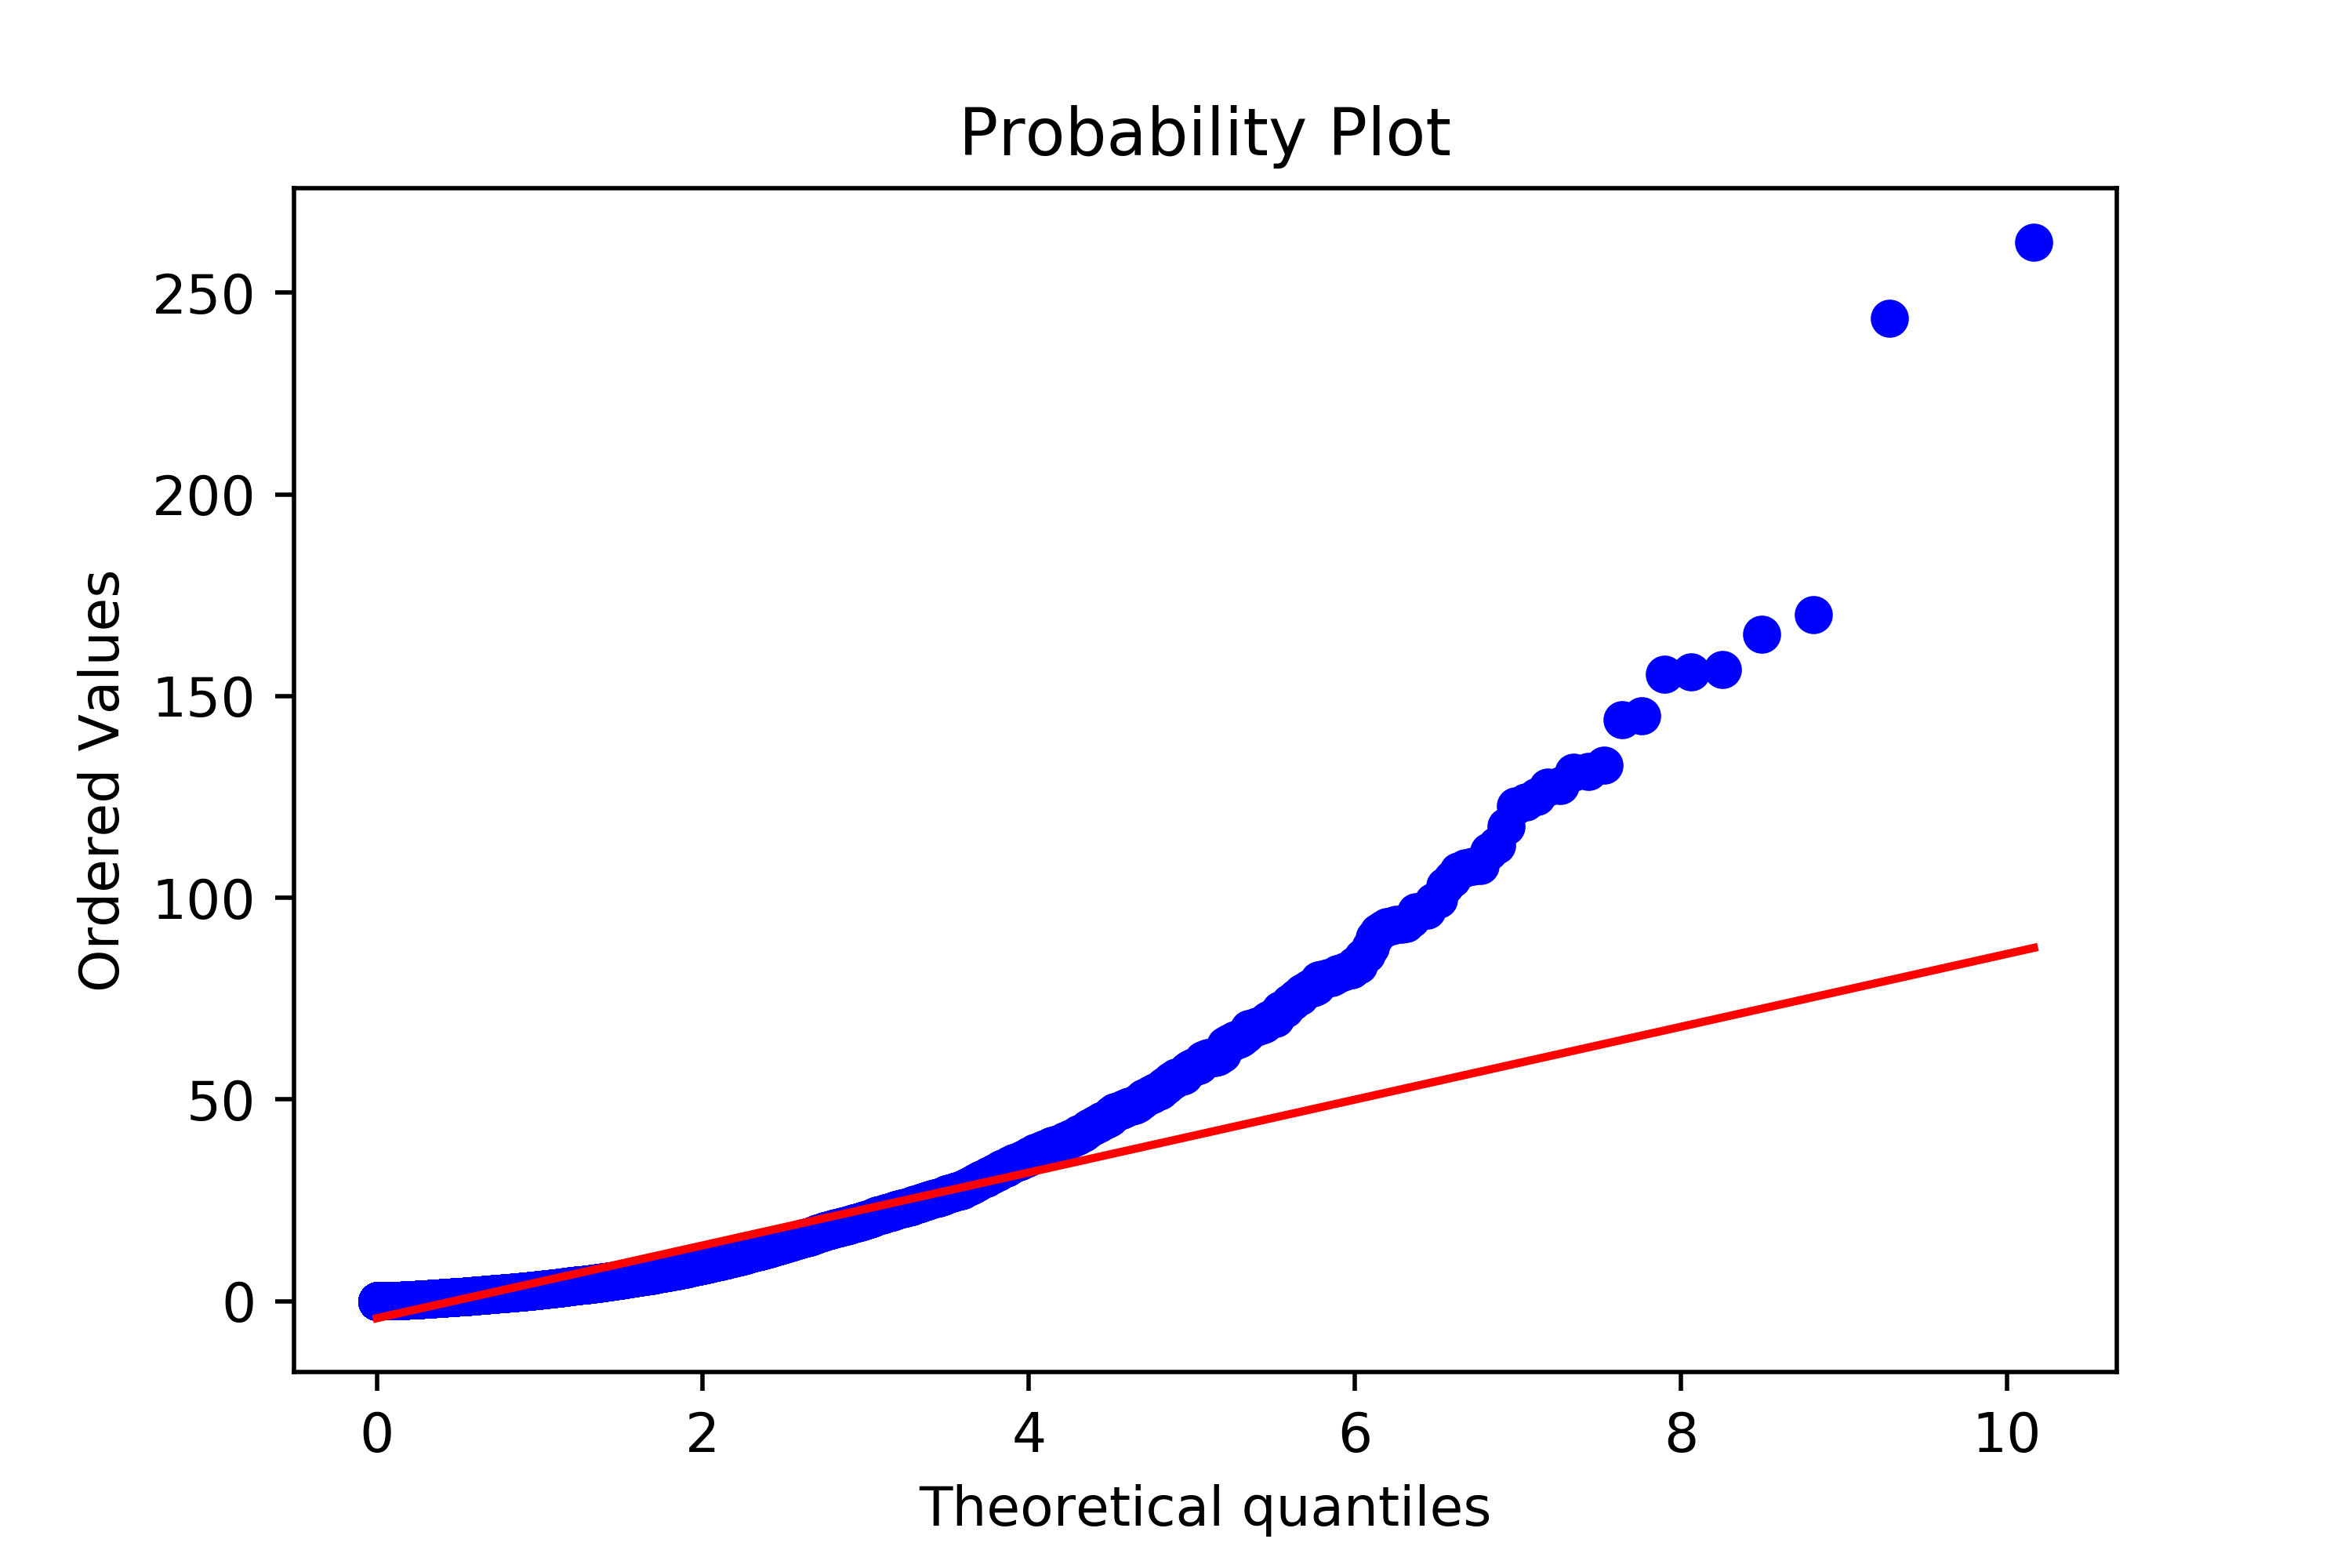
\includegraphics[width=60mm]{Figures/QQ_neg_k-1.png}}
{}
&
\subf{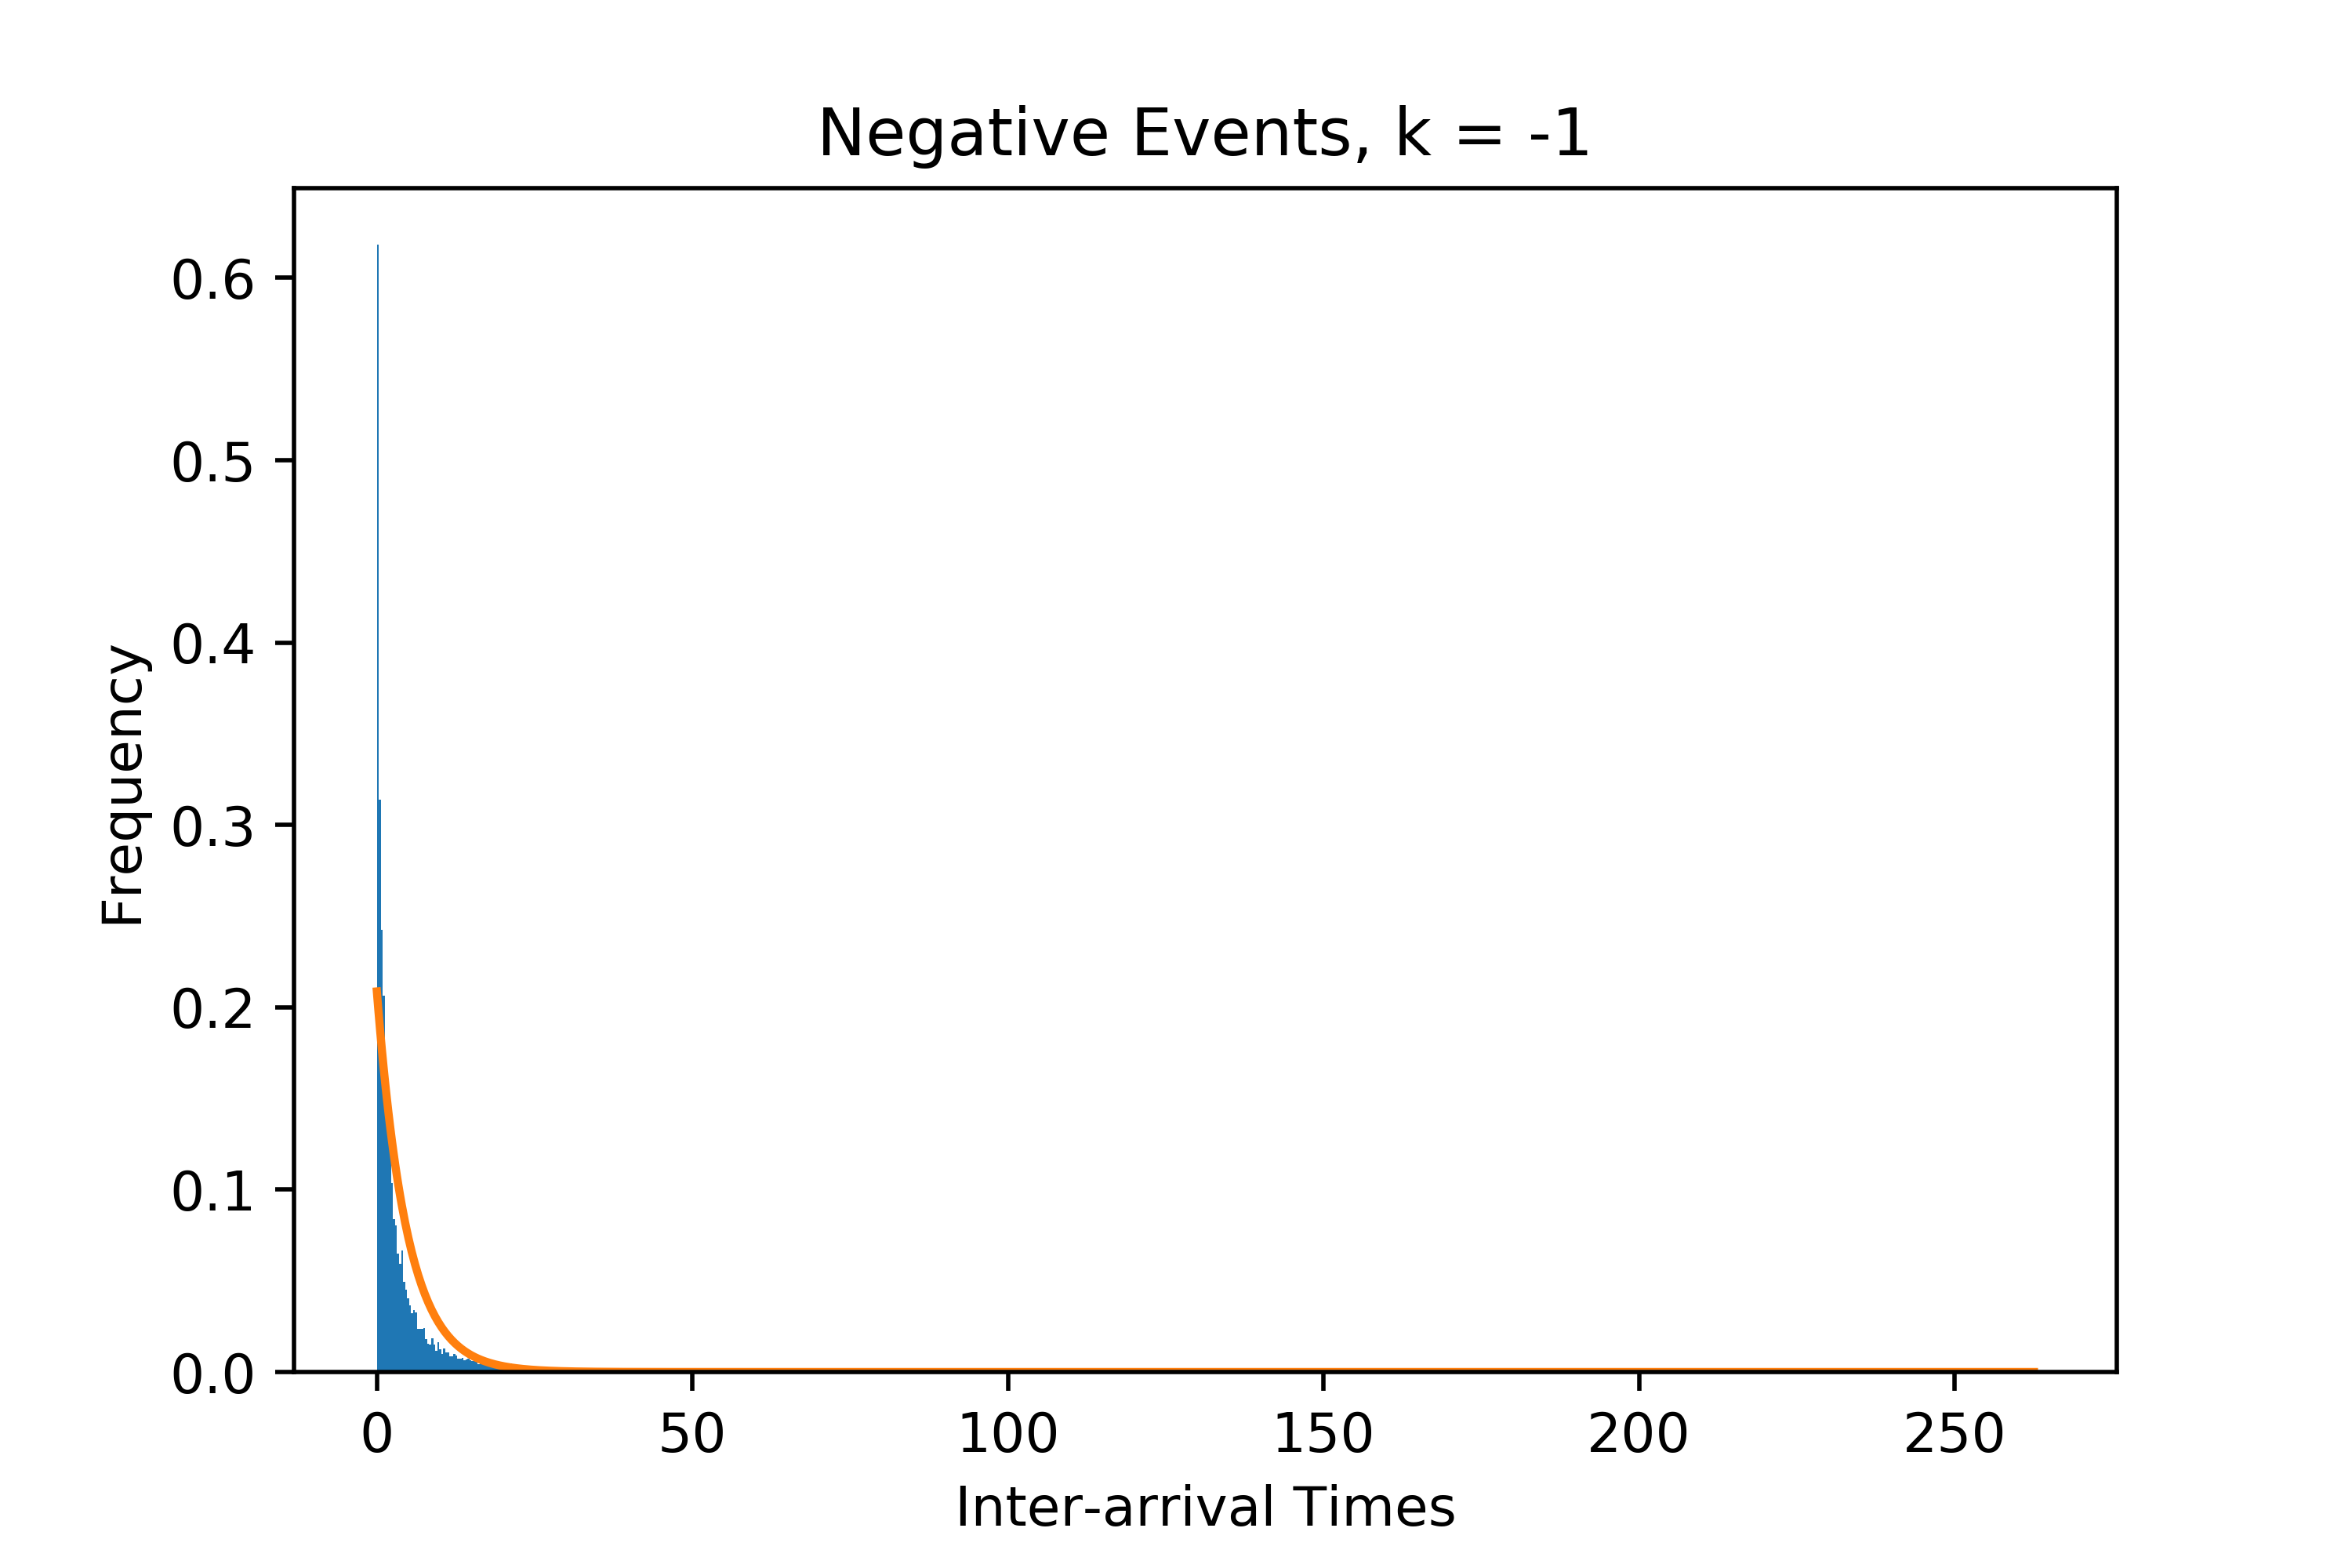
\includegraphics[width=60mm]{Figures/hist_neg_k-1.png}}
{}
\\
\subf{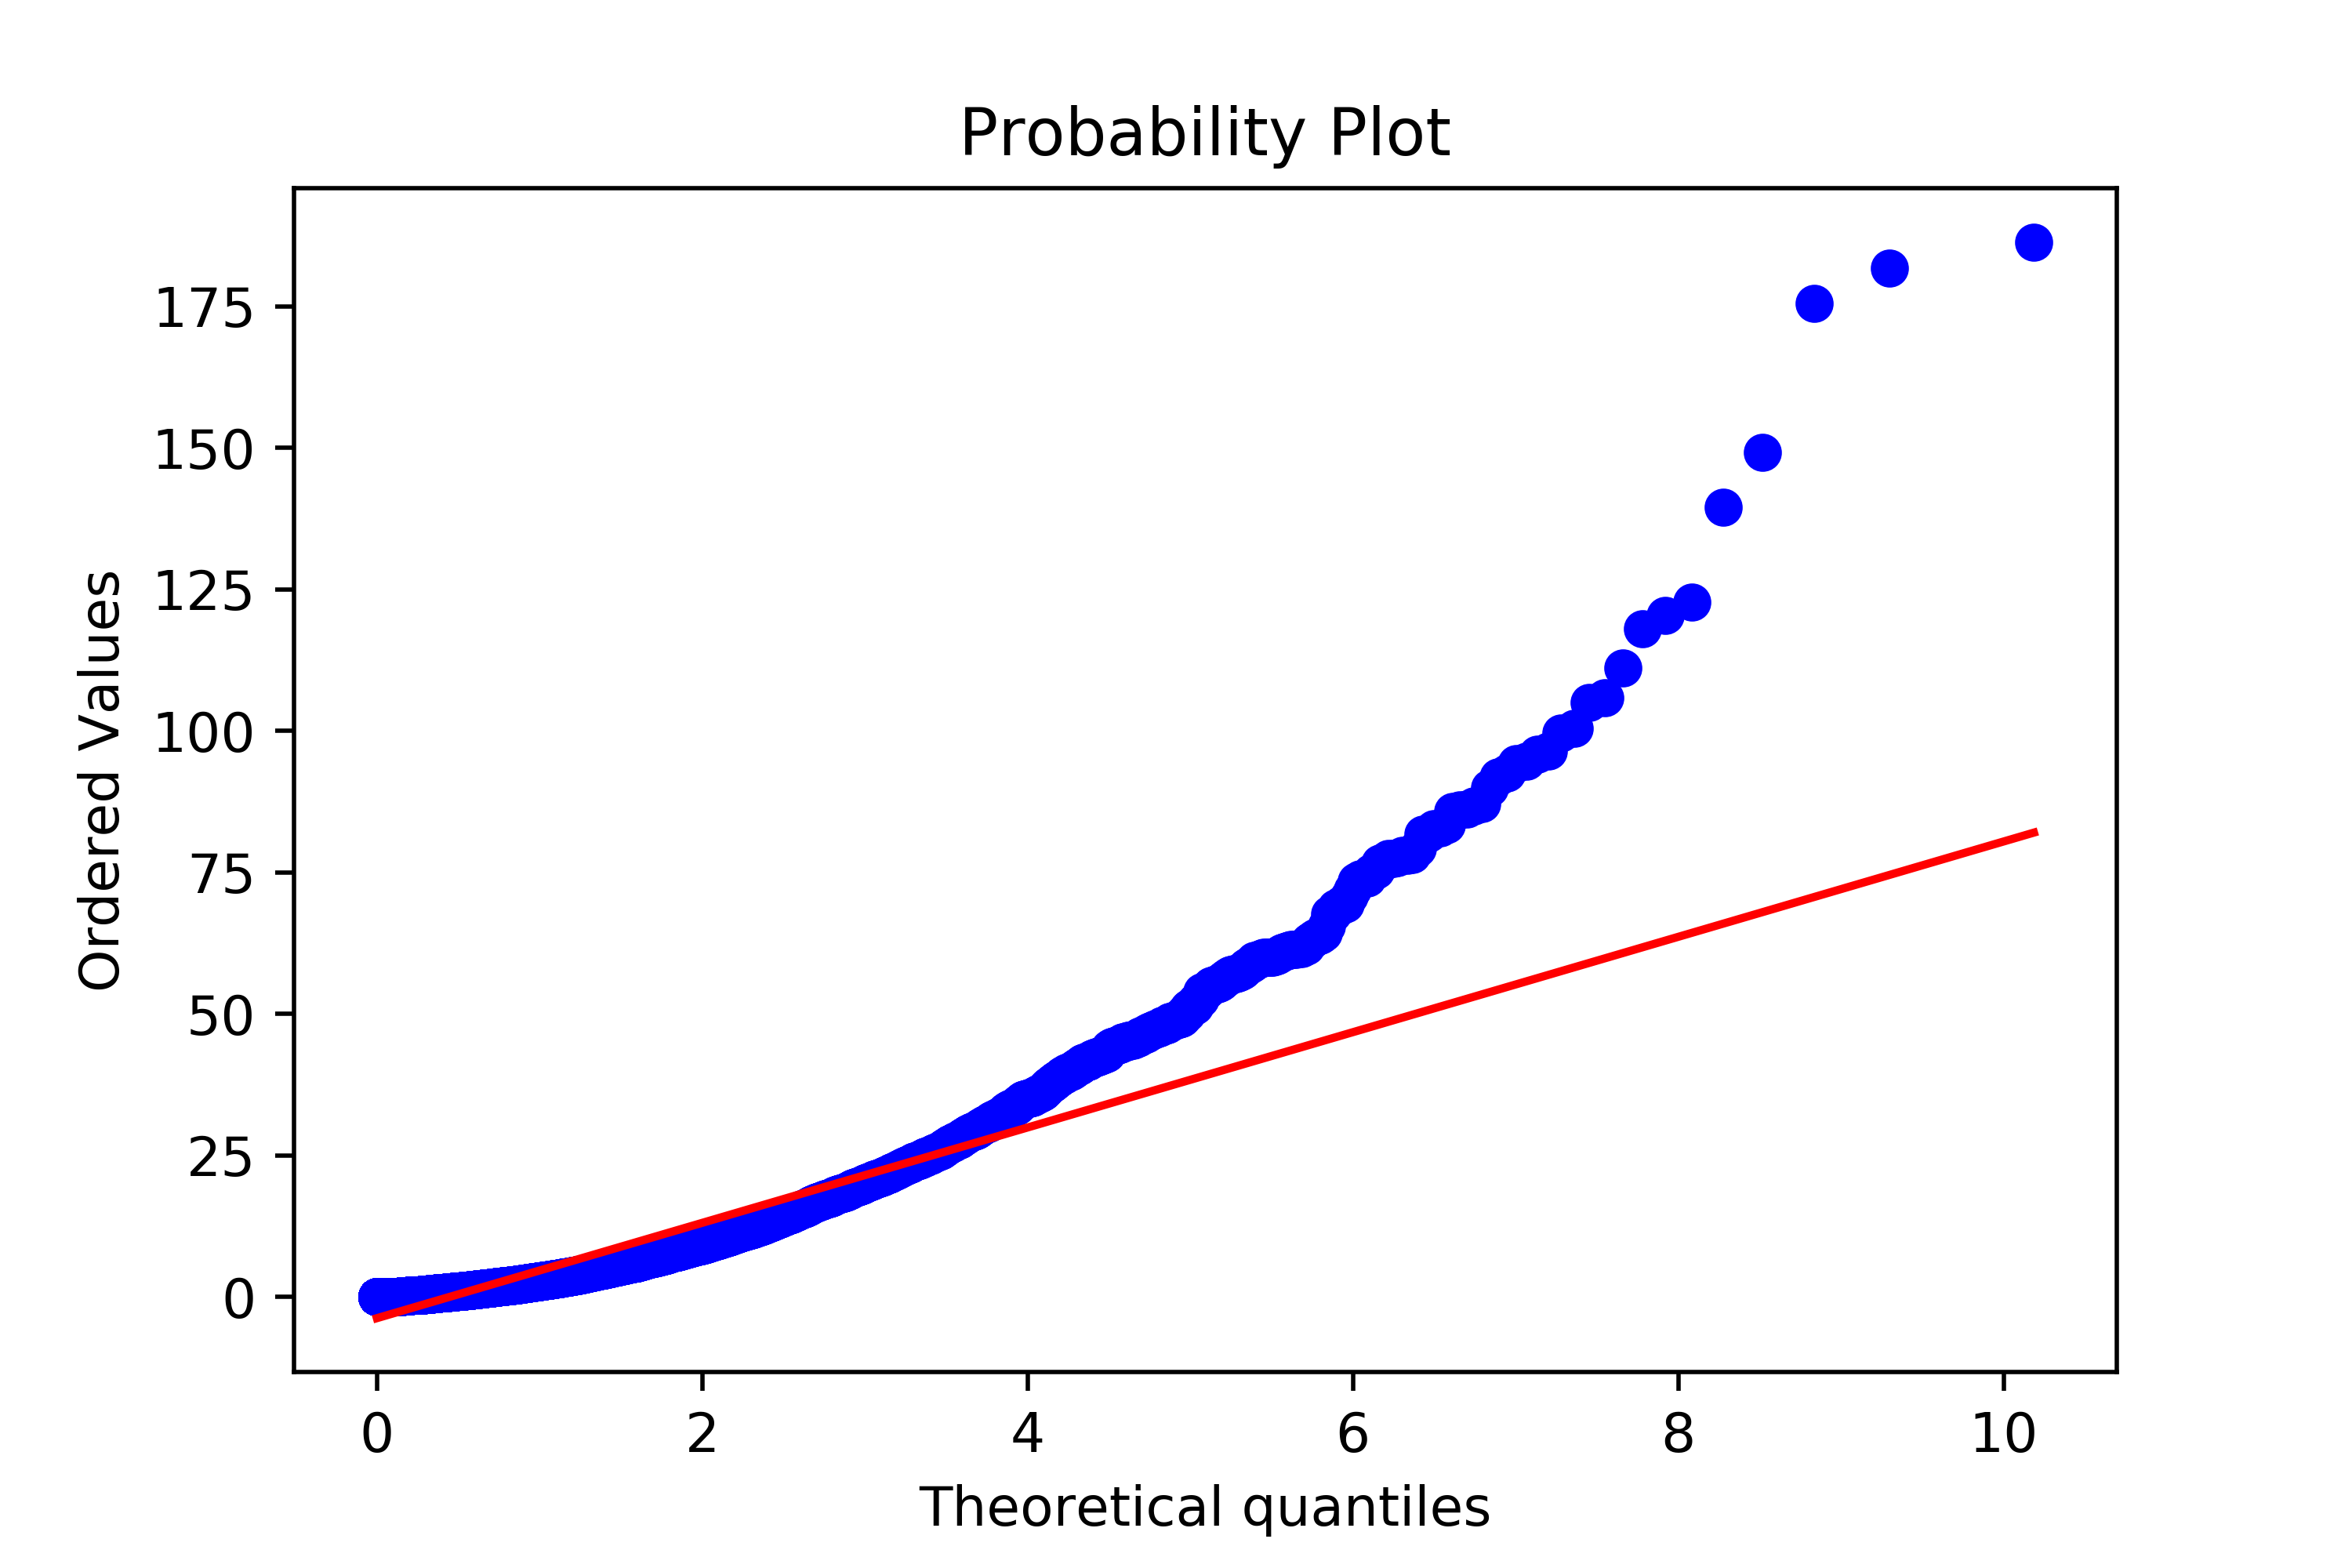
\includegraphics[width=60mm]{Figures/QQ_neg_k1.png}}
{}
&
\subf{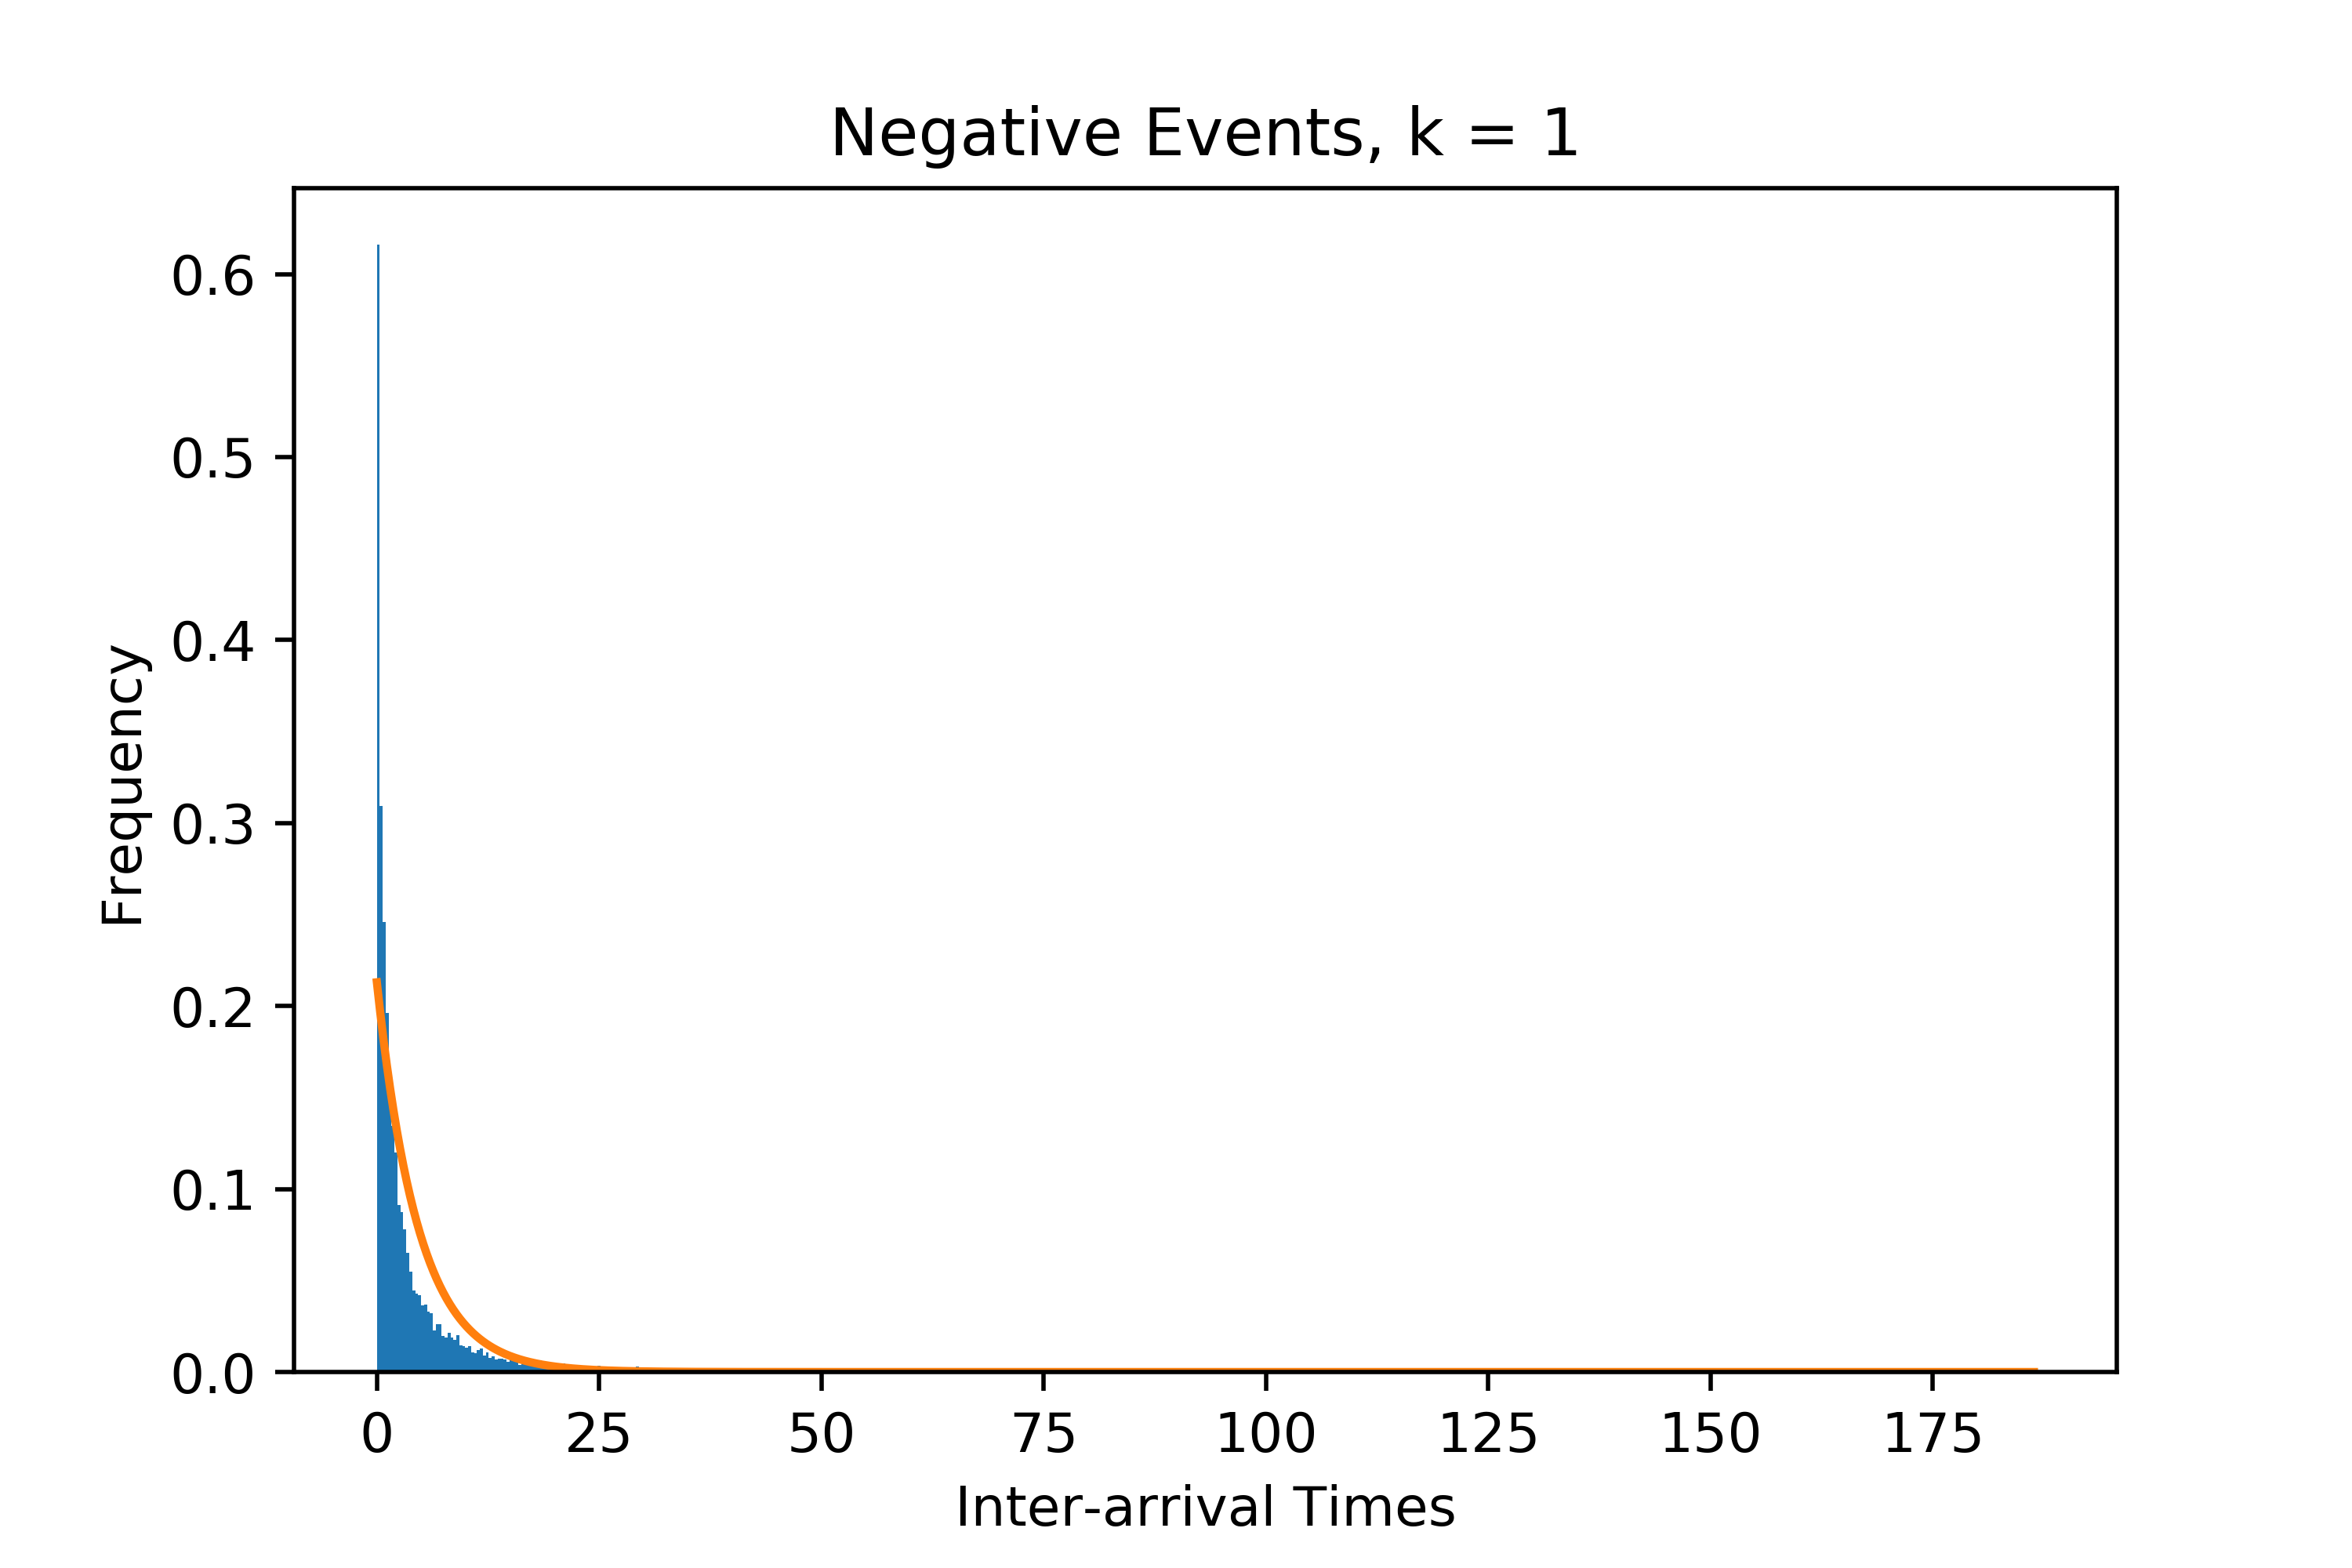
\includegraphics[width=60mm]{Figures/hist_neg_k1.png}}
{}
\\
\subf{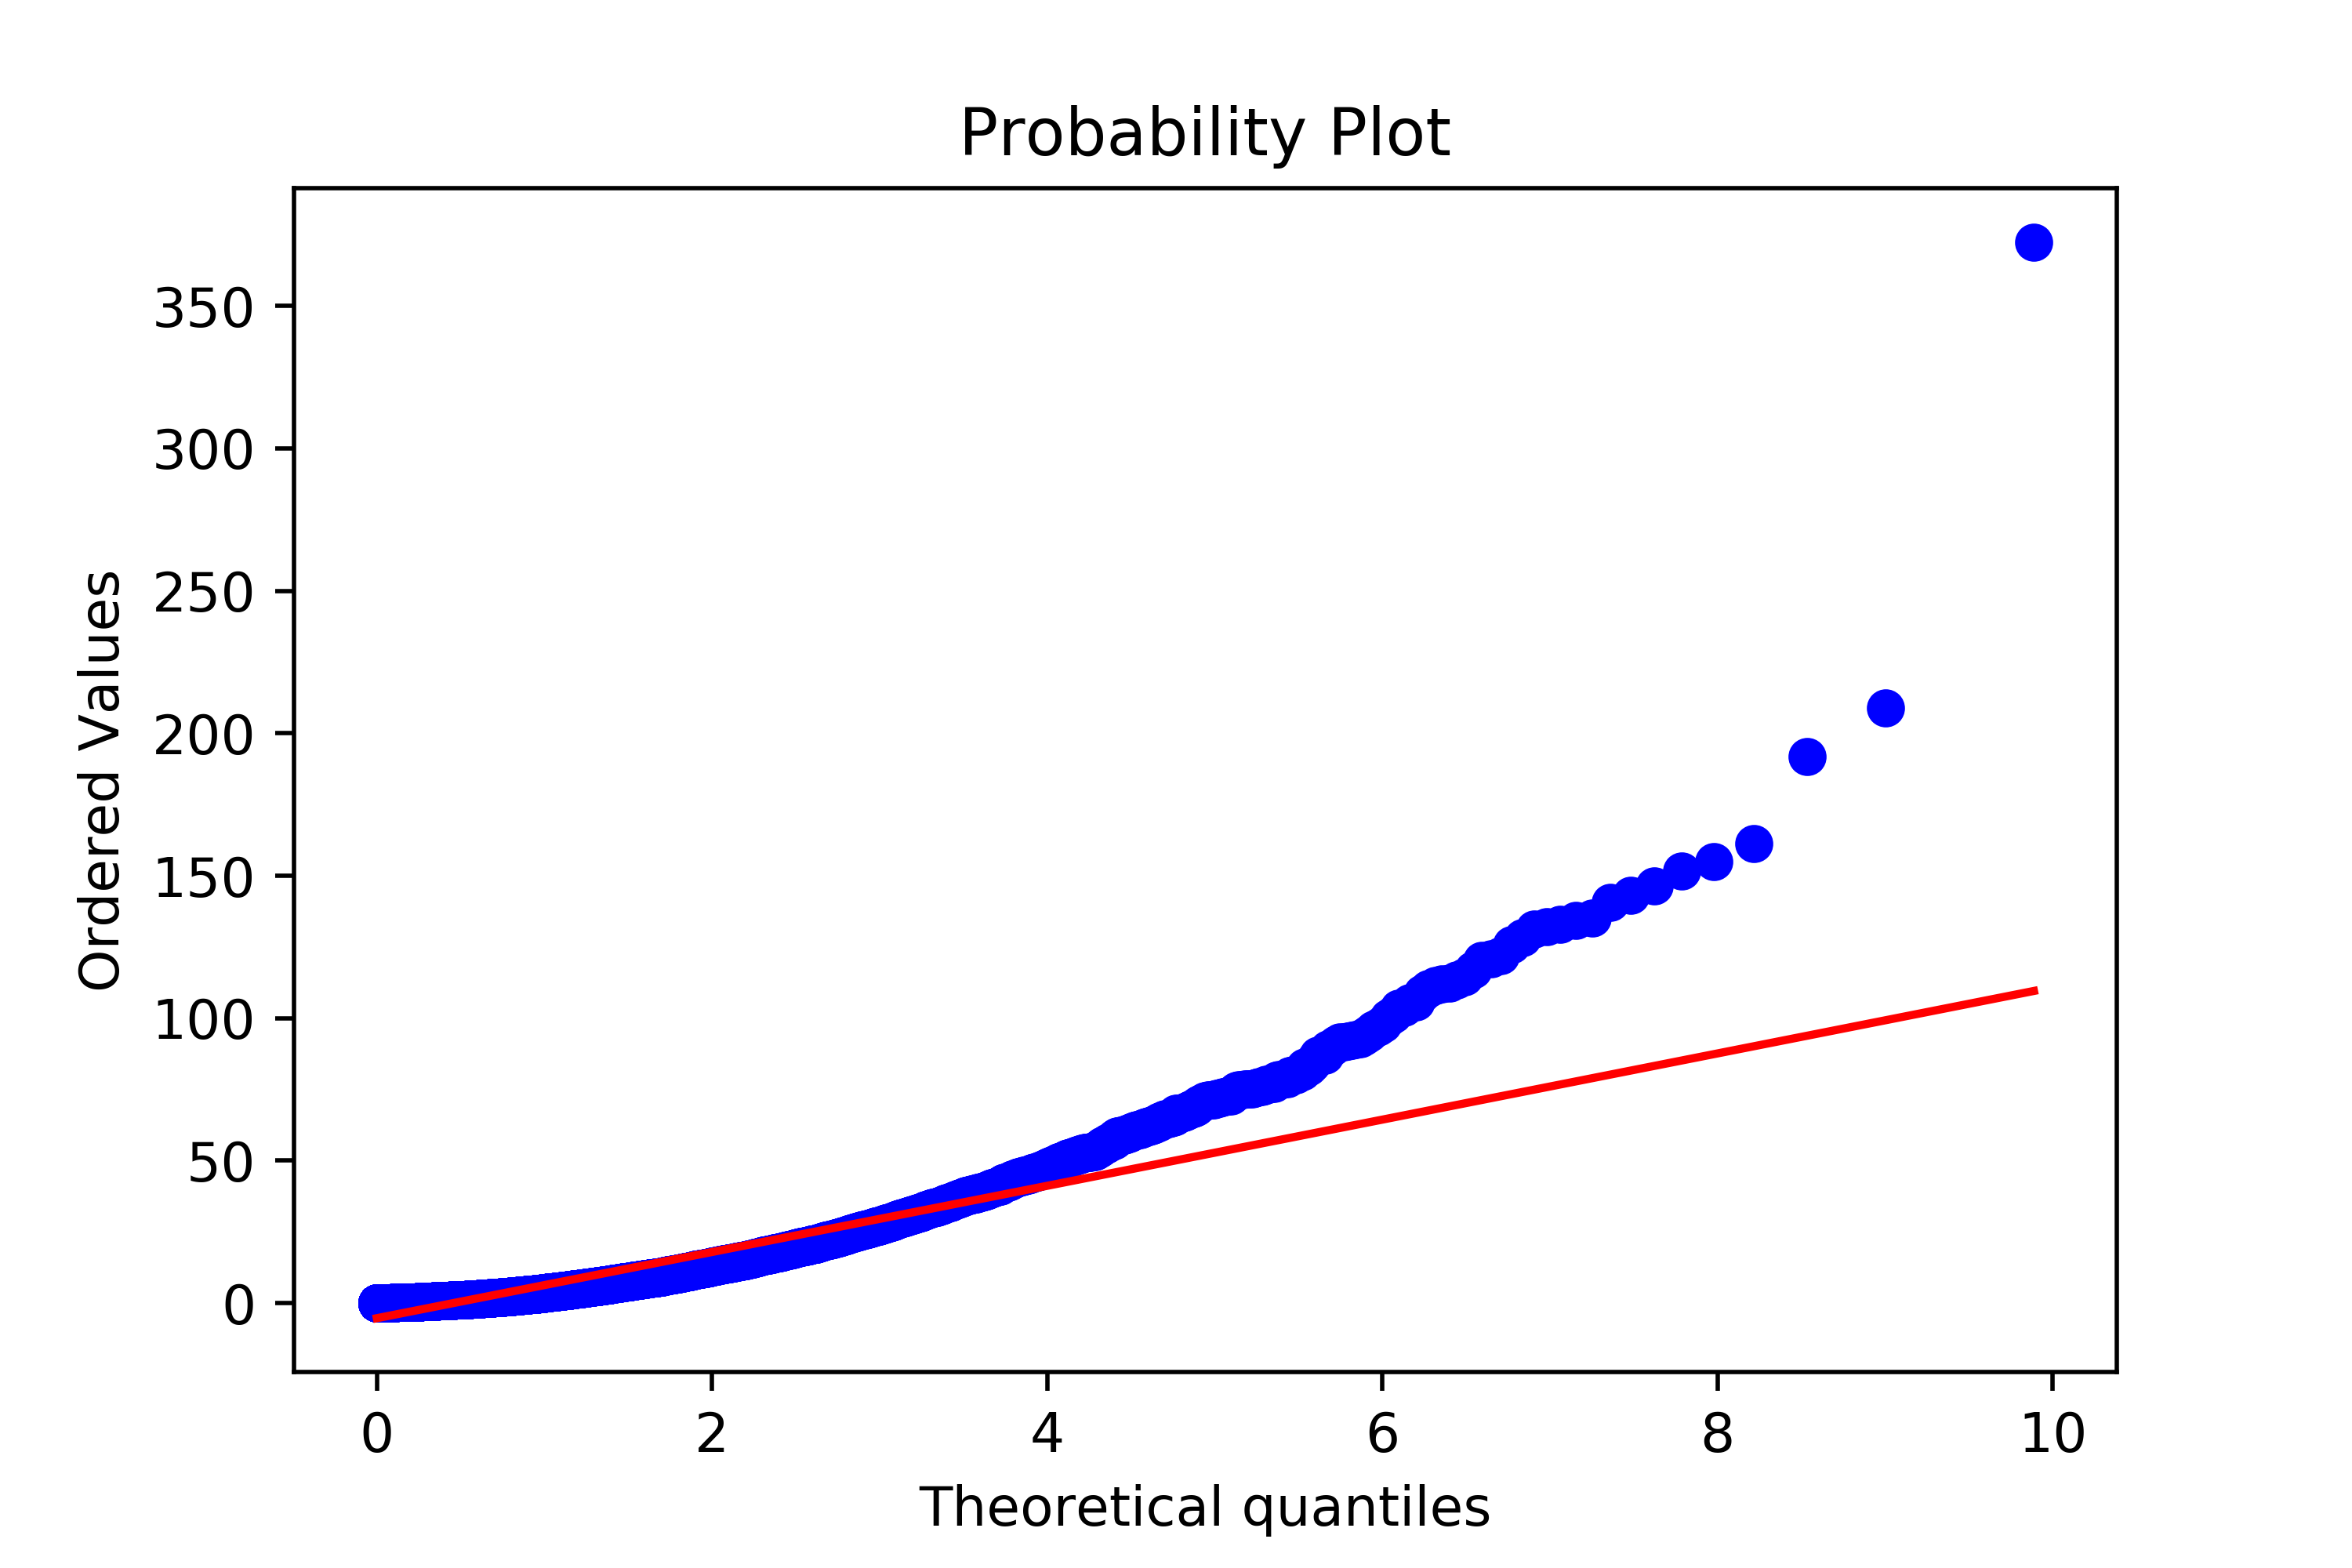
\includegraphics[width=60mm]{Figures/QQ_neg_k2.png}}
{}
&
\subf{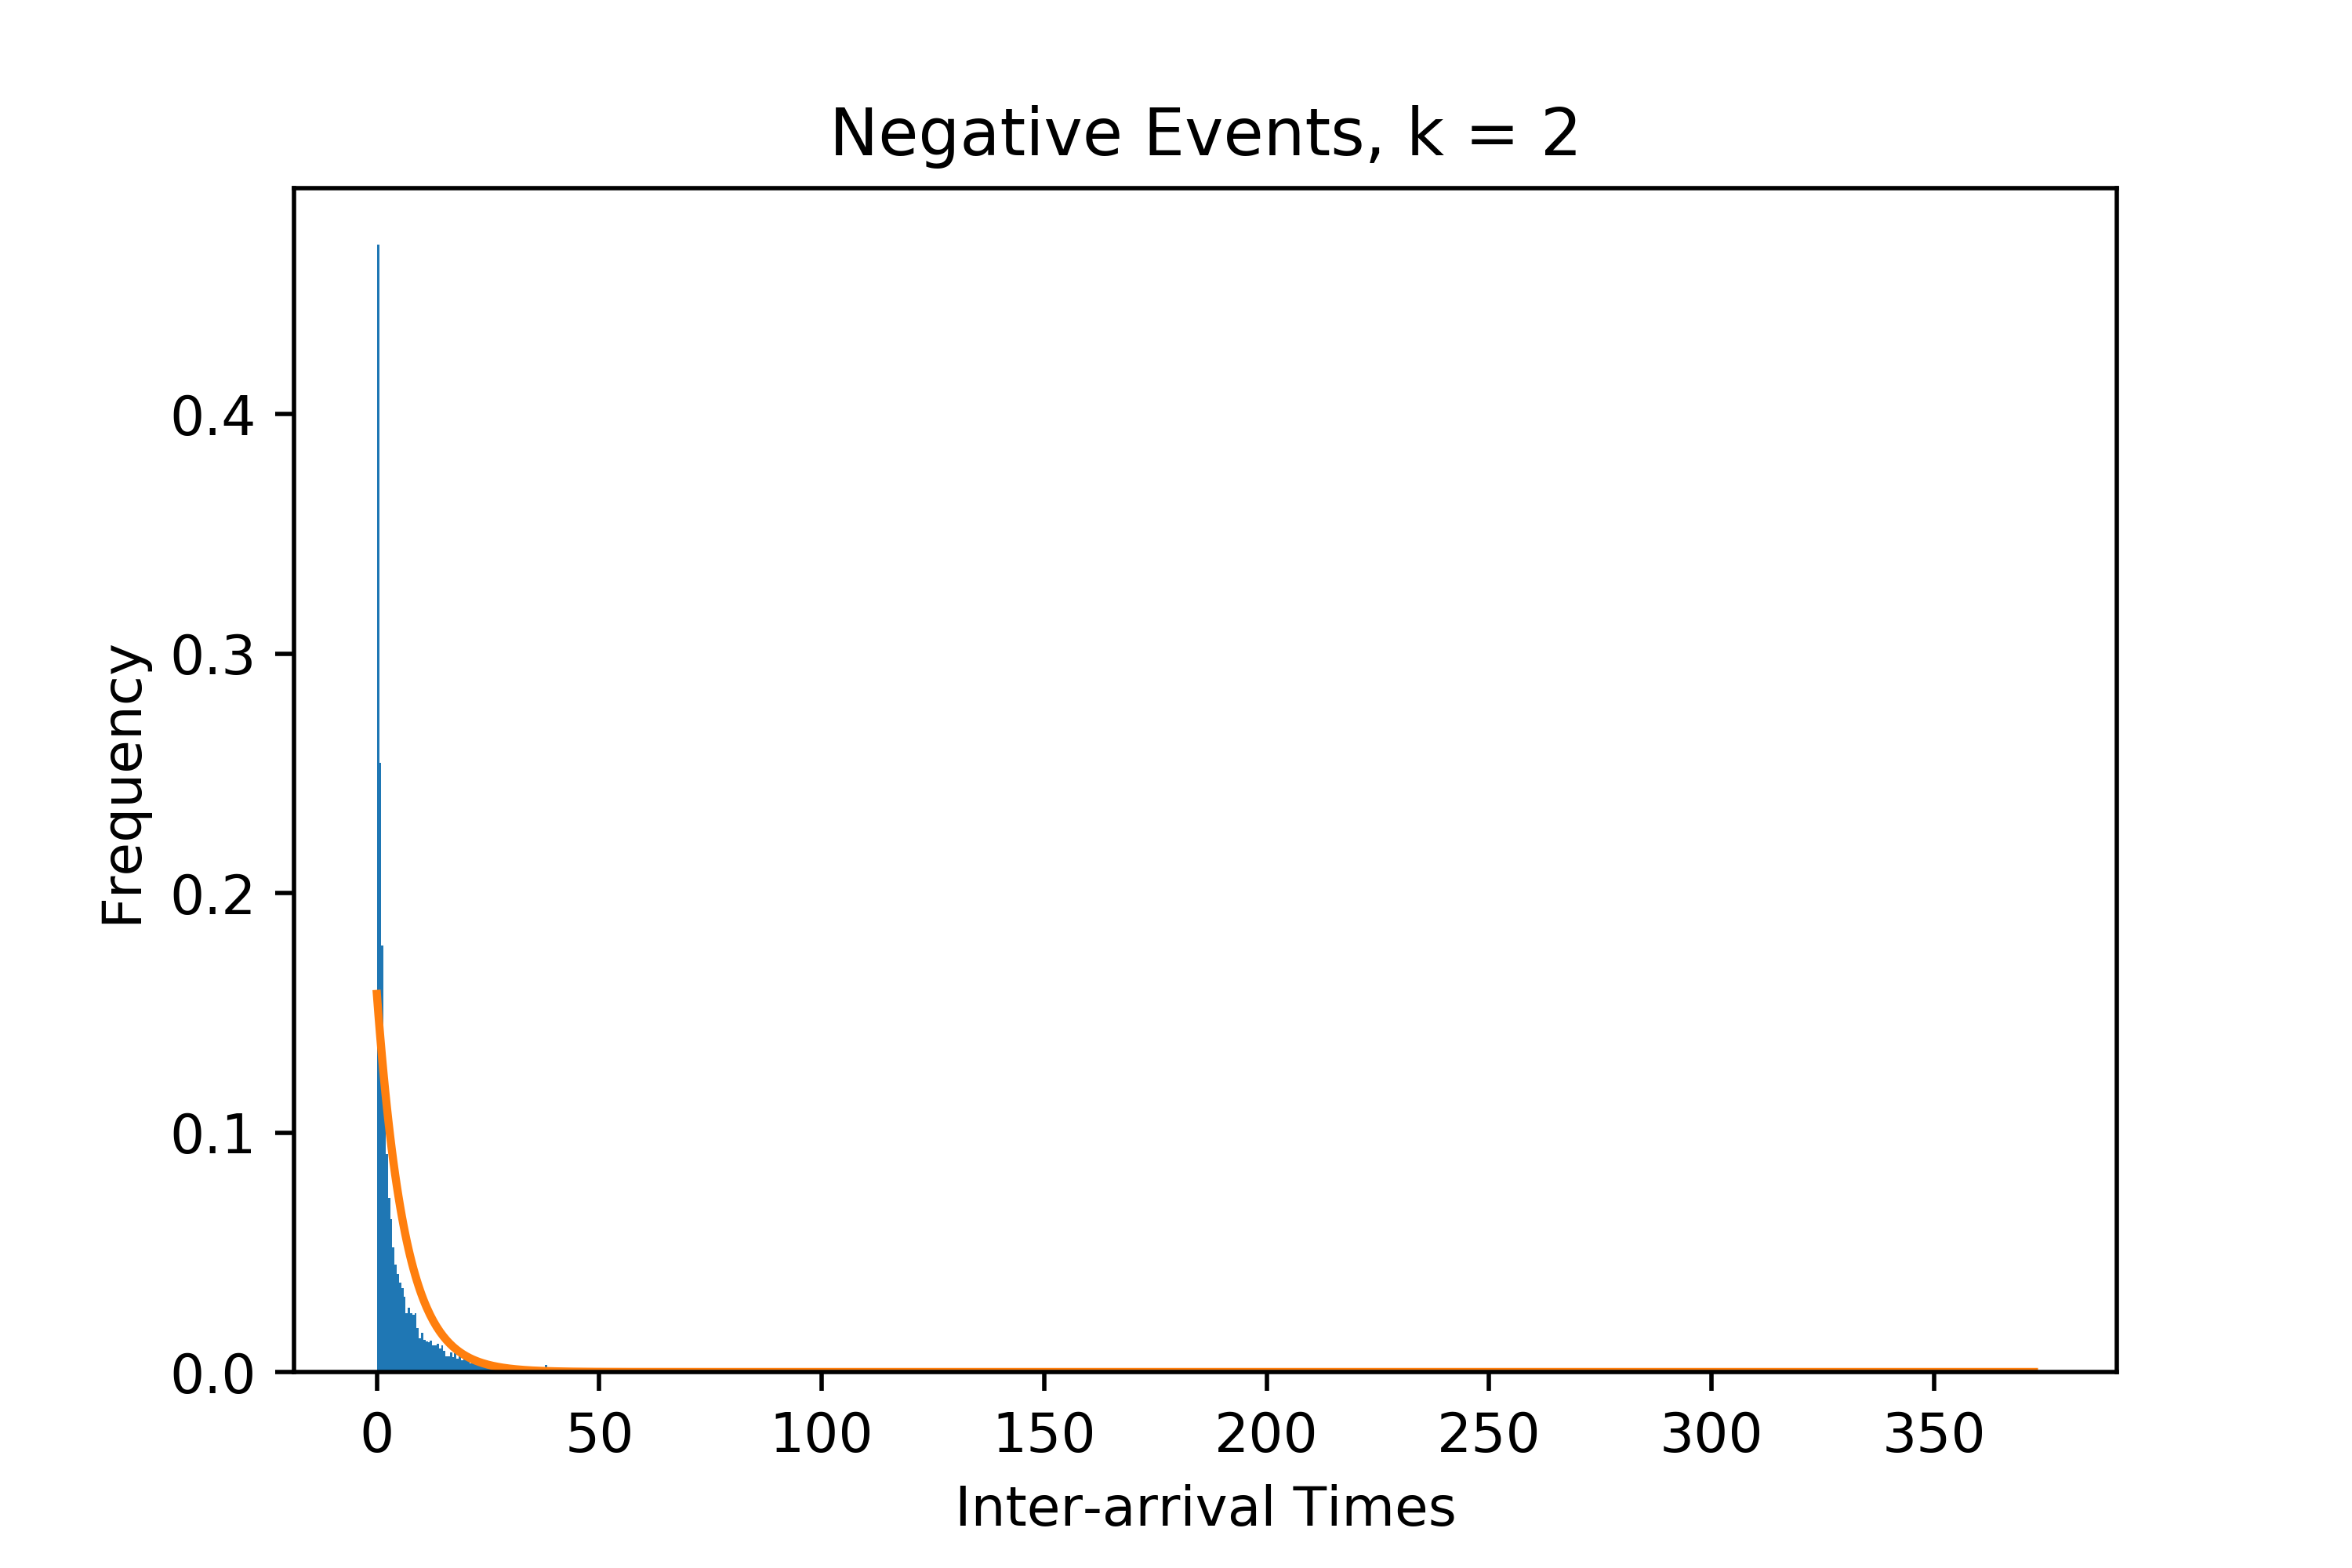
\includegraphics[width=60mm]{Figures/hist_neg_k2.png}}
{}
\\
\hline
\end{tabular}
\label{fig:interarrivals_neg}
\end{figure}

The products $\lambda^+_k \cdot \mu^+_k$ and $\lambda^-_k \cdot \mu^-_k$ can be thought of as the average rate of impact of positive and negative events at position $k$. In other words, they are the average positive and negative rates at which the size of the queue drifts over time. One concern with this model is that the impact of the positive events may overwhelm the impact of the negative events over time. That is, if $\lambda^+_k \cdot \mu^+_k > \lambda^-_k \cdot \mu^-_k$, then $Q_k(t)$ is unbounded as $t \to \infty$, which is of course unrealistic. This situation could arise due to trade imbalances in the time frame of the data that we use to estimate the parameters. We compare $\lambda^+_k \cdot \mu^+_k$ and $\lambda^-_k \cdot \mu^-_k$ in Table \ref{tab:parameters}. As can be seen, some rates are indeed larger for positive events compared to negative events. However, because the positive and negative rates are nearly the same at each position, $Q_k(t)$ should not increase an unreasonable amount in a short simulation time frame.

\section{Arrival Correlations}\label{ch:correlations}
Although each of the marginal processes can be individually modelled as a Poisson process, there were significant non-zero correlations between the numbers of arrivals at each position. Using a time period $t$ of 60 seconds, the correlations between $N^{\pm}_i(t)$ and $N^{\pm}_j(t)$ are used to generate a correlation matrix $R$ by sampling random intervals of length $t$ throughout the data collection period. With $K=10$, $R$ is a 40 x 40 matrix and is estimated with 160000 randomly selected intervals. The code written to estimate these correlations is found in Listing \ref{correlation-code}.

The correlation matrix for positive events is shown in Figure \ref{fig:pos_pos_corr_pic} where the entry $(i,j)$ is $\text{corr}(N^{+}_i(t), N^{+}_j(t))$. In general, there are high positive correlations between arrivals at a position $k$ and positions $k \pm 1$, and to a lesser extent $k \pm 2$ and $k \pm 3$. The correlations between positions near each other suggest that increased activity near a price incites similar activity in nearby prices. The smaller but significant positive correlations for positions far away from each other could be due to different levels of activity in the market at different times. For example, there may be more trading activity and therefore more events across the board during work hours vs. nighttime hours.

\begin{figure}[t]
\begin{center}
\caption{Correlation Matrix for $N^{+}_i(t), N^{+}_j(t)$, $t$ = 60 seconds}
\label{fig:pos_pos_corr_pic}
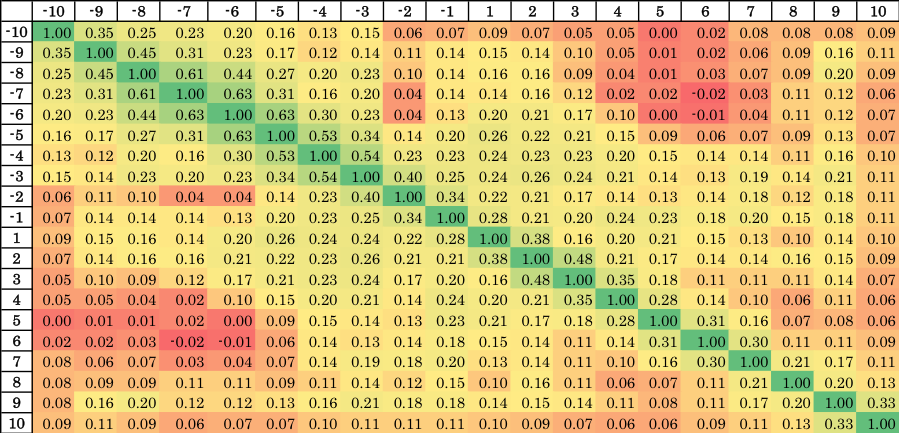
\includegraphics[width=\textwidth]{LaTeX/Figures/pos_pos_correlations.png}
\end{center}
\end{figure}

The correlation matrix for positive vs. negative events is shown in Figure \ref{fig:pos_neg_corr_pic} where the entry $(i,j)$ is $\text{corr}(N^{+}_i(t), N^{-}_j(t))$. Particularly notable is the very high (nearly 1) correlation between positive and negative arrivals at the same position. This characteristic could be due to traders reacting to updates by placing orders in the opposite direction, and could indicate that the order book is resilient to changes in the short term.

\begin{figure}[t]
\caption{Correlation Matrix for $N^{+}_i(t), N^{-}_j(t)$, $t$ = 60 seconds}
\begin{center}
\label{fig:pos_neg_corr_pic}
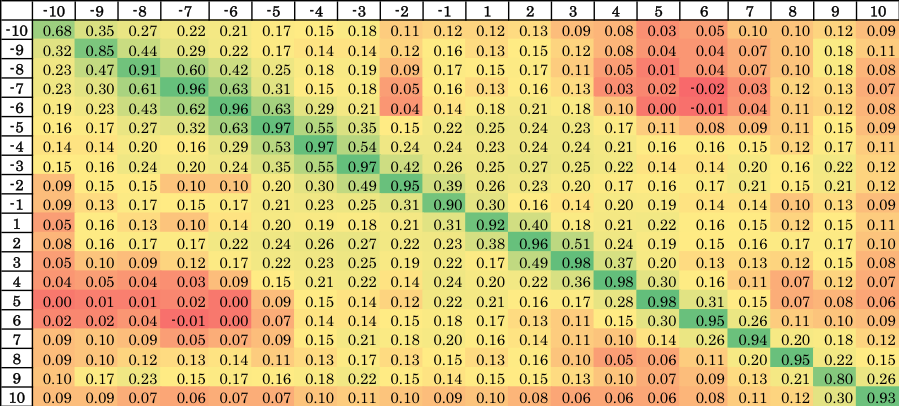
\includegraphics[width=\textwidth]{LaTeX/Figures/pos_neg_correlations.png}
\end{center}
\end{figure}

The correlation matrix for negative events is shown in Figure \ref{fig:neg_neg_corr_pic} where the entry $(i,j)$ is $\text{corr}(N^{-}_i(t), N^{-}_j(t))$. This matrix is similar in nature to the one for positive events, where positions near each other exhibit high correlations and there are lower positive correlations between positions that are further away from each other.

\begin{figure}[t]
\begin{center}
\caption{Correlation Matrix for $N^{-}_i(t), N^{-}_j(t)$, $t$ = 60 seconds}
\label{fig:neg_neg_corr_pic}
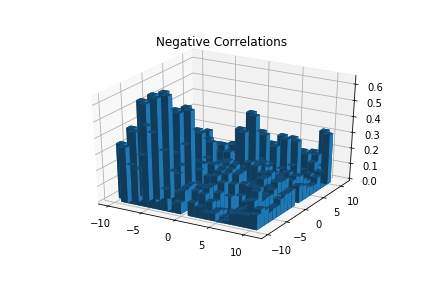
\includegraphics[width=\textwidth]{LaTeX/Figures/neg_neg_correlations.png}
\end{center}
\end{figure}

These non-zero correlations are clearly non-negligible, so a multivariate Poisson process where the arrivals are correlated and the marginal arrivals follow individual Poisson processes is appropriate. The correlations in Figures \ref{fig:pos_pos_corr_pic}, \ref{fig:pos_neg_corr_pic}, and \ref{fig:neg_neg_corr_pic} can be combined to form $R$ as described. The procedure for simulating the multivariate Poisson arrival process is discussed in Chapter \ref{ch:simulation}.


\chapter{Simulating the LOB} \label{ch:simulation}
\section{Generating Correlated Poisson Variables}\label{ch:generate_correlated_poisson}
In presenting the simulation procedure, it is necessary to discuss the method for generating correlated Poisson processes. The goal is to generate a multivariate random variable $\boldsymbol{X} = (X_1, X_2, \ldots, X_d)$ with mean $(\lambda_1, \lambda_2, \ldots, \lambda_{d})$ and $d$ x $d$ correlation matrix $R_d$ where each $X_i$ has a marginal distribution that is the same as the distribution of a Poisson variable with mean $\lambda_i$. That is, $P(X_i = x_i) = f_i(x_i)$, where $f_i$ is the probability mass function of a Poisson variable with mean $\lambda_i$. \cite{A8} describes a procedure for generating $\boldsymbol{X}$ using the copula approach. 

A copula is defined as any joint probability cumulative distribution function where each marginal distribution is uniformly distributed (\cite{B1}). That is, 

$$C(\boldsymbol{u}): [0,1]^d \to [0,1]$$ 

is a copula if $C(0, 0, \ldots, 0) = 0$ and $C(1, \ldots, 1, u_i, 1, \ldots, 1) = u_i$ and $u_i \in [0,1]$ for all $i$. The Gaussian copula as described in \cite{A8} is used, where

$$ C_R^{Gaussian}(u_1, u_2, \ldots, u_d) = \Phi_{R_d}(\Phi^{-1}(u_1), \Phi^{-1}(u_2), \ldots,  \Phi^{-1}(u_d))$$

where $\Phi$ is the cumulative distribution function for a standard random normal variable and $\Phi_{R_d}$ is the cumulative distribution function for a random multivariate normal vector with mean $0$, variance $1$, and correlation matrix $R_d$. $u$ can be generated by first generating a multivariate normal random variable $Y = (Y_1,Y_2, \ldots, Y_d)$ with correlation matrix $R_d$ and setting $(u_1, u_2, \ldots, u_d) = (\Phi(y_1), \Phi(y_2), \ldots,  \Phi(y_d))$. It can then be paired with a copula that has marginal Poisson distributions. Namely,

$$ C^{Poisson}(F_1(x_1), F_2(x_2), \ldots, F_d(x_d))$$ where $F_i$ is the discrete cumulative distribution function for a Poisson random variable with rate $\lambda_i$. $x$ can then be set to

$$(x_1, x_2, \ldots, x_d) = (F^{-1}_1(u_1), F^{-1}_2(u_2), \ldots, F^{-1}_d(u_d))$$

To implement $F^{-1}_i(u_i)$, the inverse transform method as described in \cite{B1} is used:
$$ $$

\begin{algorithm}[H]
\SetAlgoLined
\caption{Inverse Transform Method for Generating a Poisson Rate Variable With Mean $\lambda$ and quantile $u$}
 Let $i = 0$\;
 Let $p = e^{-\lambda}$\;
 Let $F = p$\;
 \While{$u \geq F$}{
  $p \leftarrow \lambda p / (i + 1)$ \;
  $F \leftarrow F + p$ \;
  $i \leftarrow i + 1$ \;
 }
 return $i$ \;
\end{algorithm}

Each $x_i$ will have a marginal Poisson distribution with rate $\lambda_i$ and $x$ will approximately have correlation matrix $R_d$. Table \ref{tab:experimental_correlation} shows the accuracy of this method for different desired correlations. For each desired correlation 10000 pairs of random variables $(x_1,x_2)$ are generated that have means $1$ and joint Poisson distribution (see Listing \ref{correlated-poisson}). For each correlation level, $x_1$ and $x_2$ have the correct means that are very near 1. For positive correlations, the actual correlation is slightly below the desired correlation (less than 0.1 difference at each desired correlation). For negative correlations, the actual correlation is slightly above the desired correlation for smaller magnitudes and deviates significantly at higher magnitudes. In practice, our correlation matrix $R$ contains values that range from small negative to large positive correlations (see Tables \ref{tab:pos_pos_corr_tab}, \ref{tab:pos_neg_corr_tab}, and \ref{tab:neg_neg_corr_tab}), so this method would generate Poisson arrivals that follow $R$ closely. It may be possible to generate arrivals that more accurately reflect the given correlations, but this method provides acceptable performance given our needs.

\begin{table}
\label{tab:experimental_correlation}
\centering
\caption{Actual vs. Desired Correlation Using Gaussian Copula, $n=10000$}
\begin{tabular}{l|l|l|l}
\hline \hline
\textbf{Desired Correlation} & $\bar{x_1}$ & $\bar{x_2}$ & \textbf{Actual Correlation}  \\ 
\hline
-1                  & 0.995                           & 1.009                           & -0.735              \\
-0.9                & 0.997                           & 0.997                           & -0.682              \\
-0.8                & 1.01                            & 0.985                           & -0.616              \\
-0.7                & 0.987                           & 1.003                           & -0.543              \\
-0.6                & 0.99                            & 1.014                           & -0.472              \\
-0.5                & 0.998                           & 1.002                           & -0.405              \\
-0.4                & 1.016                           & 0.988                           & -0.308              \\
-0.3                & 1.003                           & 1.005                           & -0.236              \\
-0.2                & 1.001                           & 1.007                           & -0.163              \\
-0.1                & 0.998                           & 1.018                           & -0.086              \\
0                   & 1.014                           & 0.986                           & 0.016               \\
0.1                 & 0.976                           & 0.992                           & 0.062               \\
0.2                 & 0.994                           & 0.986                           & 0.162               \\
0.3                 & 0.995                           & 1.002                           & 0.246               \\
0.4                 & 1.006                           & 1.004                           & 0.371               \\
0.5                 & 1                               & 0.997                           & 0.433               \\
0.6                 & 0.987                           & 1.001                           & 0.522               \\
0.7                 & 1.007                           & 1.007                           & 0.616               \\
0.8                 & 0.993                           & 0.986                           & 0.727               \\
0.9                 & 1.01                            & 1.008                           & 0.829               \\
1                   & 0.997                           & 0.997                           & 1                  
\end{tabular}
\end{table}

\section{Backwards Simulation} \label{ch:backwards_simulation}

Using the methods in Section \ref{ch:generate_correlated_poisson}, the numbers of positive and negative events in a time period of length $t$ can be generated with means equal to $\lambda^{\pm}_k \cdot t$ and correlation matrix $R$. Given the numbers of arrivals, a method called backwards simulation can be used to simulate the times of events (\cite{A7}). 

Backwards simulation uses the fact that conditioned on the number of arrivals in a Poisson process in a time period $t$ being equal to $n$, these arrivals are distributed uniformly across $[0,t)$. Using this method, arrivals over a large time period $T$ (i.e. $T = 10t$) can be generated by simulating arrivals in smaller chunks of size $t$. An algorithm is presented below for simulating arrivals over a time period $[s,s+t)$, with the arrivals following a $4K$ multivariate Poisson process with means $\lambda^{\pm}_k$ and correlation matrix $R$. The event sizes are distributed exponentially with means $\mu^{\pm}_k$ as described in Section \ref{ch:poisson}. It returns a list of events $E$ whose entries $(k,y,\tau)$ are the event position, size, and time respectively:
$$ $$

\begin{algorithm}[H]
\label{alg:backwards_simulation}
\SetAlgoLined
\caption{Backwards Simulation Method For Generating Correlated Poisson Arrivals During Time Period $[s, s+t)$}
 $E = []$;

 Generate Poisson variables $(n^{\pm}_{-K}, \ldots, n^{\pm}_{-1}, n^{\pm}_1, \ldots, n^{\pm}_K)$ with means $(\lambda^{\pm}_{-K}, \ldots, \lambda^{\pm}_{-1}, \lambda^{\pm}_1, \ldots, \lambda^{\pm}_K)$ and correlation matrix $R$ (see Section \ref{ch:generate_correlated_poisson}) \;
 
 \For{$k = -K, \ldots, -1, 1, \ldots, K$} {
    \For{$i = 1, \ldots, n^+_k$} {
        Generate $\tau$ $\sim$ Uniform($s$, $s+t$) \;
        Generate $y$ $\sim$ Exponential($\mu^+_k$) \;
        Append $(k,y,\tau)$ to $E$ \;
    }
    \For{$i = 1, \ldots, n^-_k$} {
        Generate $\tau$ $\sim$ Uniform($s$, $s+t$) \;
        Generate $y$ $\sim$ Exponential($\mu^-_k$) \;
        Append $(k,-y,\tau)$ to $E$ \;
    }
 }
 
 Return $E$ \;
 
\end{algorithm}

$$ $$

Sample arrivals using parameters estimated in Chapter \ref{ch:experiment} are shown in Figures \ref{fig:bid_events_graphs} and \ref{fig:ask_events_graphs}. Positive events are shown in blue while negative events are shown in orange.

\begin{figure}
\centering
\caption{Bid Arrivals over $T$ = 600 seconds}
\begin{tabular}{cc}
\hline
\subf{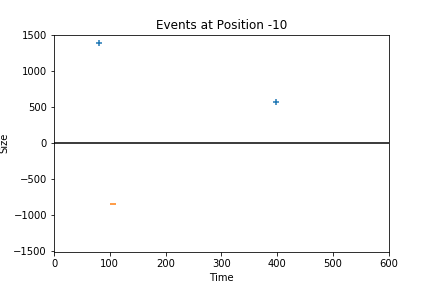
\includegraphics[width=60mm]{Figures/Events/events-10.png}}
{}
&
\subf{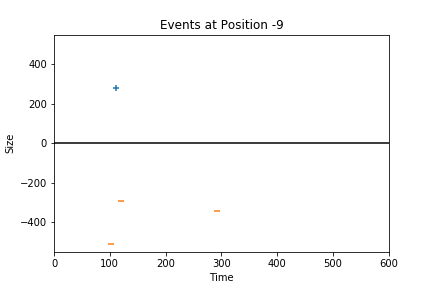
\includegraphics[width=60mm]{Figures/Events/events-9.png}}
{}
\\
\subf{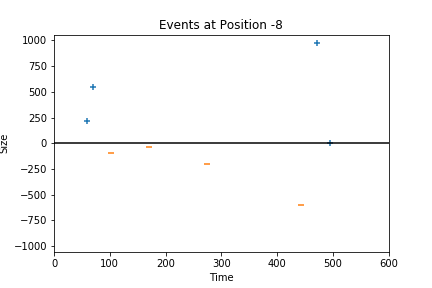
\includegraphics[width=60mm]{Figures/Events/events-8.png}}
{}
&
\subf{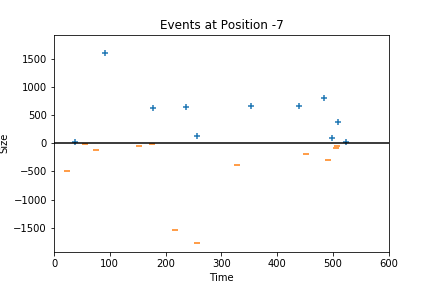
\includegraphics[width=60mm]{Figures/Events/events-7.png}}
{}
\\
\subf{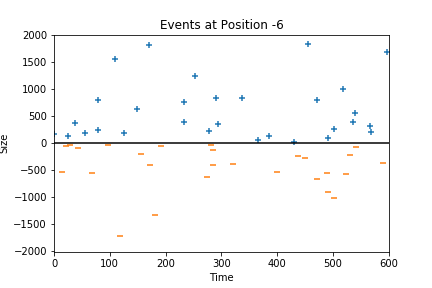
\includegraphics[width=60mm]{Figures/Events/events-6.png}}
{}
&
\subf{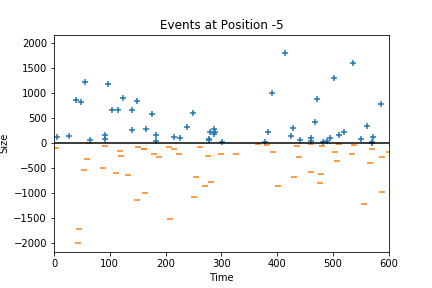
\includegraphics[width=60mm]{Figures/Events/events-5.png}}
{}
\\
\subf{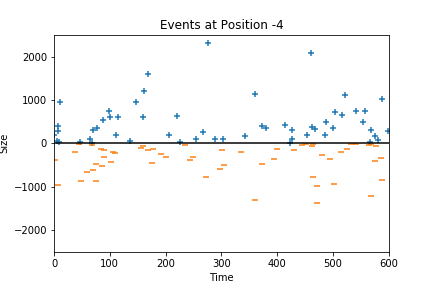
\includegraphics[width=60mm]{Figures/Events/events-4.png}}
{}
&
\subf{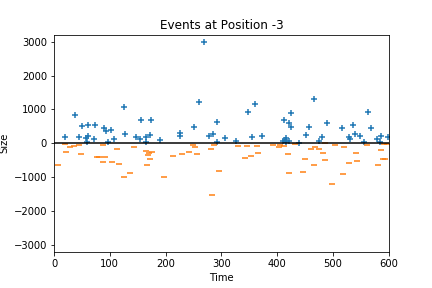
\includegraphics[width=60mm]{Figures/Events/events-3.png}}
{}
\\
\subf{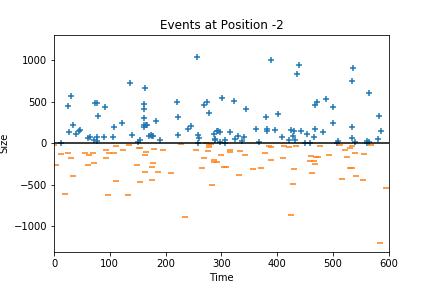
\includegraphics[width=60mm]{Figures/Events/events-2.png}}
{}
&
\subf{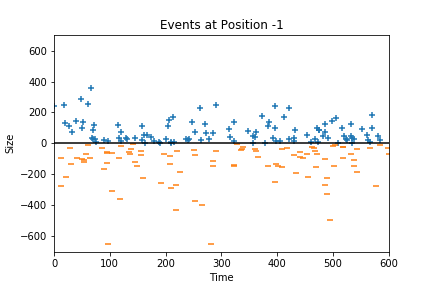
\includegraphics[width=60mm]{Figures/Events/events-1.png}}
{}
\\
\hline
\end{tabular}
\label{fig:bid_events_graphs}
\end{figure}

\begin{figure}
\centering
\caption{Ask Arrivals over $T$ = 600 seconds}
\begin{tabular}{cc}
\hline
\subf{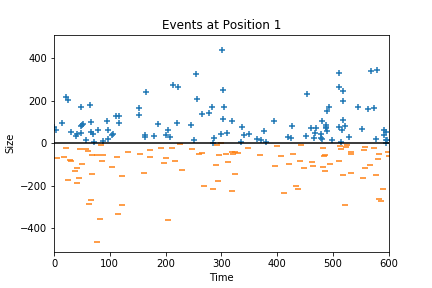
\includegraphics[width=60mm]{Figures/Events/events1.png}}
{}
&
\subf{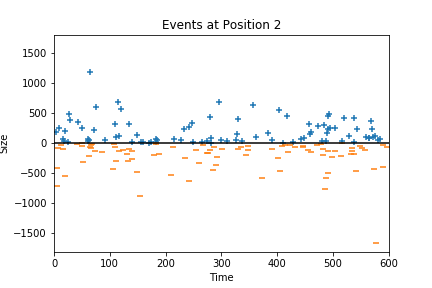
\includegraphics[width=60mm]{Figures/Events/events2.png}}
{}
\\
\subf{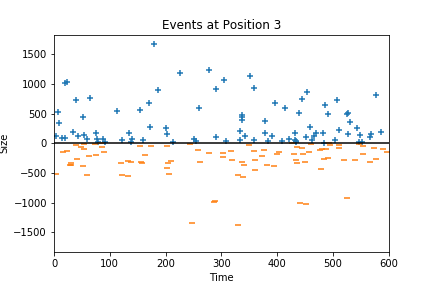
\includegraphics[width=60mm]{Figures/Events/events3.png}}
{}
&
\subf{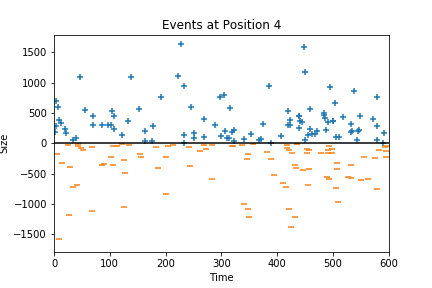
\includegraphics[width=60mm]{Figures/Events/events4.png}}
{}
\\
\subf{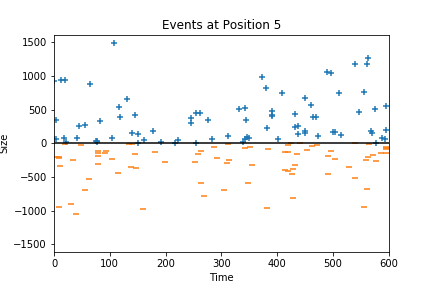
\includegraphics[width=60mm]{Figures/Events/events5.png}}
{}
&
\subf{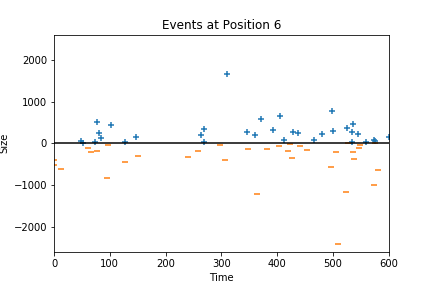
\includegraphics[width=60mm]{Figures/Events/events6.png}}
{}
\\
\subf{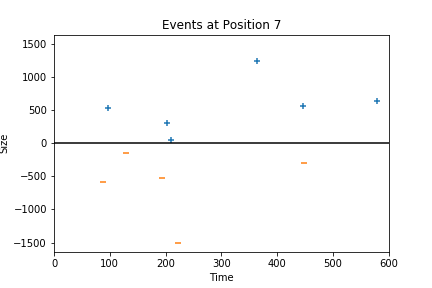
\includegraphics[width=60mm]{Figures/Events/events7.png}}
{}
&
\subf{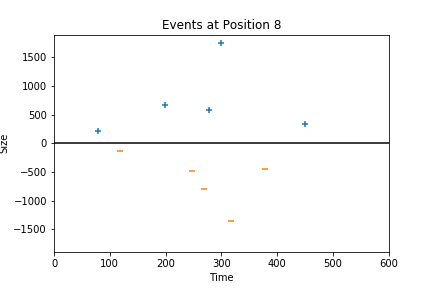
\includegraphics[width=60mm]{Figures/Events/events8.png}}
{}
\\
\subf{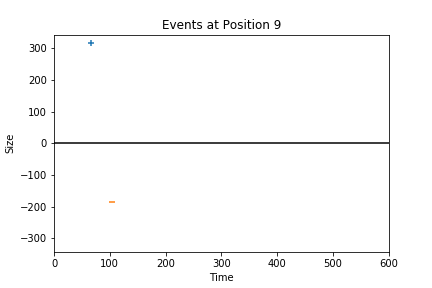
\includegraphics[width=60mm]{Figures/Events/events9.png}}
{}
&
\subf{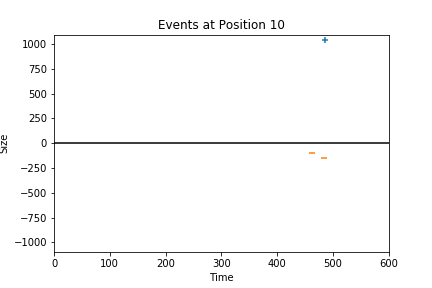
\includegraphics[width=60mm]{Figures/Events/events10.png}}
{}
\\
\hline
\end{tabular}
\label{fig:ask_events_graphs}
\end{figure}

\section{Simulation Algorithm} \label{ch:simulation_algorithm}

The actions of the agent can now be incorporated into the simulation. The agent must buy $V$ units in a time period $T$. It follows a trading schedule $\Omega$, which is a list of market orders of the form $(M,\tau)$ where $M$ is the size of the order and $\tau$ is the time at which it is to be sent. If $V$ units have not been acquired at the end of the time period, the agent makes a market order for the remainder of the inventory to comply with the spirit of the game. LOB events outside of the agent's orders are generated using Algorithm \ref{alg:backwards_simulation}, and the reference price is updated as described in Section \ref{ch:queue_model}. The simulation algorithm is presented below. It returns $\Theta$, a list of executed trades of the form $(p,a,\tau)$, which contains the price, number of units, and time of the trade.

$$ $$

\begin{algorithm}[H]
\SetAlgoLined
\caption{LOB Simulation: Setup and Input}
Let $p_0$ be the starting reference price \;

Let $L$ be the initial LOB. Let $L_p$ be the volume at price $p$ \;

Let $v$ be the amount of inventory filled \;

Let $\Theta = []$ be the trades executed \;

Let $\Omega$ be the list of market orders in the trading schedule. If $\sum\limits_\Omega{M} < V$, append $(V - \sum\limits_\Omega{M}, T)$ to $\Omega$ \;

Generate $E$ using Algorithm \ref{alg:backwards_simulation} \;

Sort $\Omega$ and $E$ by $\tau$;
\end{algorithm}

\begin{algorithm}[H]
\SetAlgoLined
\caption{LOB Simulation: Recording Executed Trades}
Proceed through $\Omega$ and $E$ in time order. 

\While{$\tau <= T$ and $v < V$} {
    \If {$\text{\upshape event of form}$ $(k,c,\tau)$} {
        Update $L$ and $p_0$ (see Section \ref{ch:queue_model}) \;
    }
    \If {$\text{\upshape order of form}$ $(M,\tau)$} {
        Let $p = p_0 + 0.5$ \;
        \While {$L_p$ = 0} {
            $p \leftarrow p + 1$
        }
        Let $m = M$ \;
        \While {$m > 0$} {
            Let $a = (L_p - m)^+$ \;
            
            $L_p \leftarrow L_p - a$ \;
            
            Append $(p, a, \tau)$ to $\Theta$ \;

            $m \leftarrow m - a$ \;
    
            $p \leftarrow p + 1$ \;
        }
        $v \leftarrow v + M$ \;
        
        Update $p_0$ \;
    }
}

Return $\Theta$ ;
\end{algorithm}

$$ $$

$\Theta$ can then be used to compute the VWAP performance of the trading schedule. See Listing \ref{code:simulation} for the code written to perform the simulation.

\chapter{Evaluating Trade Execution Performance} \label{ch:trade_execution}
The simulated market environment can be used to assess the performance of a given trade execution strategy. Using this procedure, the agent can adjust its strategy to acquire its inventory goal at the most favorable price before executing the trade in reality. Section \ref{ch:strategies} provides an overview of common algorithmic trade execution strategies. Section \ref{ch:sim_results} evaluates the performance of the TWAP and VWAP strategies (see Subsection \ref{ch:impact-driven}) in the simulated market environment.

\section{Trade Execution Strategies} \label{ch:strategies}
Trade execution strategies can be broadly classified into impact-driven, cost-driven, and opportunistic algorithms (\cite{labadie:hal-00590283}). Nuanced trading strategies can be created using a combination of these algorithms.

\subsection{Impact-Driven Algorithms} \label{ch:impact-driven}
Impact-driven algorithms seek to minimize the market impact of a large trade by splitting it into slices of smaller trades over time. 

Time Weighted Average Price (TWAP) algorithms split a large order of size $V$ into $n$ smaller orders of size $V/n$ uniformly over a time period $T$. In order to reduce predictability and prevent detection by third parties, modifications of TWAP where the size and timing of orders are slightly varied are often preferred. When simulating TWAP performance, the default TWAP strategy is used, assuming that no third party takes action upon detecting our TWAP strategy and that the market reacts as it normally would to our trades.

Volume Weighted Average Price (VWAP) algorithms are similar to TWAP algorithms, but they divide the time period $T$ into sub-periods where the volume of market activity measurably differs. The size of the orders during each sub-period is proportional to its volume of market activity during that sub-period. The volume of market activity in each sub-period is typically predicted using historical data. VWAP strategies theoretically lower market impact compared to TWAP strategies by sending larger orders when there is more market activity (and thus higher LOB resiliency) and smaller orders when there is less market activity. However, they run the risk of incurring significantly higher execution costs if the historical data does not reflect market activity at the time of execution. The VWAP trading strategy should not be confused with the VWAP benchmark used to measure the performance of trade execution (Chapter \ref{ch:intro}).

Percentage of Volume algorithms (POV), like VWAP, generate sizes of orders based on trading volume throughout the time period. However, they trade a fixed percentage of the current market volume based on a desired participation rate. For example, the agent may choose to submit orders so that are expected to comprise 5\% of the market activity in the period. Unlike the TWAP and VWAP algorithms that follow fixed trading schedules, POV algorithms have dynamically determined trading schedules.

\subsection{Cost-Driven Algorithms}
Cost-driven algorithms seek to minimize transaction costs, including market impact and market timing risks. In addition to market impact consideration taken in the impact-driven algorithms above, cost-driven algorithms adjust the time horizon of trades to account for market timing risks (i.e. orders for more volatile assets are executed in a shorter time horizon). Implementation Shortfall algorithms attempt to minimize the difference between the price at which the investor decides to make the trade and the average price at which the trade is executed. Market Close algorithms are similar to Implementation Shortfall algorithms, but the benchmark of comparison is the closing price.

\subsection{Opportunistic Algorithms}
Opportunistic algorithms seek to take advantage of favorable market conditions. Price Inline algorithms dynamically adjust trading patterns in response to the asset price (i.e. increasing trading activity when the price is low). Liquidity Driven algorithms take into account order book depth and availability of venues for trading. Pair Trading algorithms consist of buying one asset and selling another. If the assets are sufficiently correlated, the risks from one asset balance out the risks from the other. Pair Trading takes advantage of mean-reverting behavior to generate profit.


\section{Trade Execution Simulation} \label{ch:sim_results}
In this section, the performance of TWAP and VWAP strategies are tested in the simulated market environment.
\subsection{The Initial LOB}
To begin with an LOB that is representative of the market, the reference price is set to the time weighted average price of the asset rounded to the nearest mid-price. The volumes at the first $K=10$ surrounding bid and ask prices are set to the time weighted average volumes at those positions, and the volumes at other positions are set to 100. The LOB is maintained as simulation proceeds. The starting book is shown in Table \ref{tab:starting_LOB}.

\begin{table}[htbp]
\caption{Starting LOB for Simulation. $p_0 = 516.5$ cents} \label{tab:starting_LOB}
\begin{center}
\begin{tabular}{ll|ll}
\hline \hline
\multicolumn{2}{l|}{\textbf{Bids}} & \multicolumn{2}{l}{\textbf{Asks}} \\
\hline
Volume        & Price    & Price      & Volume      \\
\hline
587.93       & 516       & 517        & 495.79      \\
1425.68      & 515       & 518        & 983.24      \\
2328.27      & 514       & 519        & 1475.59     \\
2735.44      & 513       & 520        & 2170.60     \\
2578.26      & 512       & 521        & 2456.86     \\
1338.90      & 511       & 522        & 1807.16     \\
609.82       & 510       & 523        & 817.16      \\
292.86       & 509       & 524        & 420.61      \\
250.14       & 508       & 525        & 404.11      \\
287.13       & 507       & 526        & 390.99             
\end{tabular}
\end{center}
\end{table}

\subsection{TWAP Strategy}
As described in Subsection \ref{ch:impact-driven}, the TWAP strategy consists of splitting the large trade into equally-sized smaller trades uniformly across the time period. The TWAP strategy is tested with a total trade size of $V = 40000$ over a period of $T = 10$ minutes and different numbers of orders to split the trade into.  An example is shown in Table \ref{tab:twap_order} where the trade is split into 8 orders of size 5000. As can be seen, the trade pushes the market price up while it is executed. The best ask price at the time of the first order is 517 and the best ask price at the time of the last order is 528 for a VWAP price of 524.820, about 8 cents higher than the starting reference price. See Listing \ref{code:twap_code} for the code written to simulate the orders resulting from a trade using the TWAP strategy.

\begin{table}[htbp]
\begin{center}
\caption{TWAP Strategy Order Example} \label{tab:twap_order}
\begin{tabular}{l|l|l|l}
\hline \hline
\multicolumn{4}{c}{\textbf{VWAP Price}: 524.820}                                      \\
\hline
\textbf{Time}                    & \textbf{Order Size}        & \textbf{Price} & \textbf{Volume}   \\
\hline
\multirow{5}{*}{66.67}  & \multirow{5}{*}{5000} & 517   & 682.696  \\
                        &                          & 518   & 428.594  \\
                        &                          & 519   & 2566.022 \\
                        &                          & 520   & 1301.644 \\
                        &                          & 521   & 21.044   \\
\hline                   
\multirow{5}{*}{133.33} & \multirow{5}{*}{5000} & 520   & 260.565  \\
                        &                          & 521   & 1454.826 \\
                        &                          & 522   & 2239.506 \\
                        &                          & 523   & 490.201  \\
                        &                          & 524   & 554.901  \\
\hline                            
\multirow{4}{*}{200.00} & \multirow{4}{*}{5000} & 522   & 62.550   \\
                        &                          & 523   & 133.966  \\
                        &                          & 524   & 3165.501 \\
                        &                          & 525   & 1637.983 \\
\hline                        
\multirow{5}{*}{266.67} & \multirow{5}{*}{5000} & 521   & 302.563  \\
                        &                          & 522   & 411.777  \\
                        &                          & 523   & 584.960  \\
                        &                          & 524   & 3541.595 \\
                        &                          & 525   & 159.105  \\
\hline                        
\multirow{3}{*}{333.33} & \multirow{3}{*}{5000} & 524   & 684.054  \\
                        &                          & 525   & 981.617  \\
                        &                          & 526   & 3334.330 \\
\hline                        
\multirow{4}{*}{400.00} & \multirow{4}{*}{5000} & 525   & 891.352  \\
                        &                          & 526   & 1403.401 \\
                        &                          & 527   & 1557.507 \\
                        &                          & 528   & 1147.739 \\
\hline                        
\multirow{4}{*}{466.67} & \multirow{4}{*}{5000} & 526   & 631.725  \\
                        &                          & 527   & 2759.918 \\
                        &                          & 528   & 1236.733 \\
                        &                          & 529   & 371.624  \\
\hline                        
\multirow{3}{*}{533.33} & \multirow{3}{*}{5000} & 528   & 461.628  \\
                        &                          & 529   & 583.475  \\
                        &                          & 531   & 3954.897
\end{tabular}
\end{center}
\end{table}

The TWAP strategy was then tested with different numbers of orders in the trading schedule. Each trading schedule was tested 10000 times with the same starting LOB. The results are shown in Table \ref{tab:twap_strategy}.

\begin{table}[htbp]
\begin{center}
\caption{TWAP Strategy Performance} \label{tab:twap_strategy}
\begin{tabular}{l|l}
\hline \hline
\textbf{No. Orders} & \textbf{Mean VWAP Price (Standard Error)} \\
\hline
1                & 573.481 (0.084)            \\
2                & 566.053 (0.116)            \\
3                & 558.112 (0.130)            \\
4                & 551.222 (0.139)            \\
5                & 542.895 (0.136)            \\
6                & 536.191 (0.120)            \\
7                & 531.526 (0.096)            \\
8                & 529.286 (0.081)            \\
9                & 529.482 (0.082)            \\
10               & 528.490 (0.070)            \\
100              & 529.318 (0.061)           
\end{tabular}
\end{center}
\end{table}

As can be seen for this particular trade size, splitting the trade into a higher number of orders significantly lowers the mean cost up to about 8 orders. Looking at the standard errors, the variability of performance generally decreases as the number of orders increases (with the exception of using just one order). Although increasing the number of orders reduces average trading cost and risk, it has drawbacks in that it may incur extra costs from exchange commissions and is more easily detectable. These simulation results are useful for an agent looking to find the optimal number of slices to use in its TWAP strategy. 

\subsection{VWAP Strategy}
As described in \ref{ch:impact-driven}, the VWAP strategy consists of splitting trades like the TWAP strategy, but determining order sizes in proportion to the volume of market trades during different sub-periods. To simulate an environment with varying levels of trading activity, the 10 minute period is split in half, where a certain proportion $\alpha$ ($0 < \alpha < 1$) of the activity occurs in the first half and $1-\alpha$ of the activity occurs in the second half. 

In order to maintain the same average volume of trades over the entire period, the rate of arrival $\lambda_k$ at a given position is adjusted as shown in Table \ref{tab:adjusted_rates}.

\begin{table}[htbp]
\caption{Adjusted Rates for VWAP Strategy Simulation} \label{tab:adjusted_rates}
\begin{center}
\begin{tabular}{l|l}
\textbf{Subperiod}            & \textbf{Adjusted Rate}             \\
\hline
First Half  & $2 \alpha \lambda_k $    \\
Second Half & $2 (1 - \alpha) \lambda_k$
\end{tabular}
\end{center}
\end{table}

In the first half of a time period $T$, the expected number of arrivals will be 
$$2 \alpha \lambda_k T / 2 = \alpha \lambda_k T$$ 
and the expected number of arrivals in the second half will be 
$$2 (1-\alpha) \lambda_k T / 2 = (1-\alpha) \lambda_k T$$
for a total of $$\lambda_k T$$

Thus, on average, $\alpha$ proportion of arrivals will occur in the first half and $1-\alpha$ proportion of arrivals occur in the second half with the same average total number of arrivals as the constant rate case. The size of the orders will be adjusted in the same way. It should be noted that these trading conditions are somewhat unrealistic. Although it is possible that trading volume could differ significantly in a short time period, it is unlikely that the agent would be able to accurately and uniquely predict such a drastic change and act upon it. Nevertheless, this analysis shows the possibility of testing the performance of a trading strategy in a simulated environment with varying rates of market activity. Table \ref{tab:vwap_order} shows an example of the orders executed with a VWAP strategy split into 8 slices when $\alpha = 0.75$, where the size of the orders in the first half is 7500 and the size of the orders in the second half is 2500. Again, the price is pushed up. The best ask price at the time of the last order is 528 and the VWAP price is 522.507, about 6 cents higher than the starting reference price. See Listing \ref{code:vwap_code} for the code written to simulate the orders resulting from trades using the VWAP strategy.

\begin{table}[htbp]
\begin{center}
\caption{VWAP Strategy Order Example, $\alpha = 0.75$} \label{tab:vwap_order}
\begin{tabular}{l|l|l|l}
\hline \hline
\multicolumn{4}{c}{\textbf{VWAP Price}: 522.507}                                      \\
\hline
\textbf{Time}                    & \textbf{Order Size}        & \textbf{Price} & \textbf{Volume}   \\
\hline
\multirow{4}{*}{66.67}  & \multirow{4}{*}{7500} & 517 & 1071.610 \\
                        &                       & 519 & 1907.321 \\
                        &                       & 520 & 4116.339 \\
                        &                       & 521 & 404.731  \\
\hline
\multirow{3}{*}{133.33} & \multirow{3}{*}{7500} & 518 & 2145.428 \\
                        &                       & 521 & 4555.106 \\
                        &                       & 522 & 799.466  \\
\hline
\multirow{6}{*}{200.00} & \multirow{6}{*}{7500} & 518 & 207.043  \\
                        &                       & 519 & 856.150  \\
                        &                       & 520 & 1513.202 \\
                        &                       & 521 & 835.556  \\
                        &                       & 522 & 1043.699 \\
                        &                       & 523 & 3044.349 \\
\hline
\multirow{5}{*}{266.67} & \multirow{5}{*}{7500} & 521 & 507.424  \\
                        &                       & 522 & 2825.699 \\
                        &                       & 523 & 1860.746 \\
                        &                       & 524 & 1134.190 \\
                        &                       & 525 & 1171.941 \\
\hline
\multirow{3}{*}{333.33} & \multirow{3}{*}{2500} & 524 & 516.300  \\
                        &                       & 525 & 1676.603 \\
                        &                       & 526 & 307.097  \\
\hline
\multirow{3}{*}{400.00} & \multirow{3}{*}{2500} & 525 & 968.908  \\
                        &                       & 527 & 759.657  \\
                        &                       & 528 & 771.434  \\
\hline
\multirow{4}{*}{466.67} & \multirow{4}{*}{2500} & 525 & 357.558  \\
                        &                       & 526 & 71.188   \\
                        &                       & 527 & 807.992  \\
                        &                       & 528 & 1263.263 \\
\hline
\multirow{3}{*}{533.33} & \multirow{3}{*}{2500} & 528 & 639.090  \\
                        &                       & 529 & 117.624  \\
                        &                       & 530 & 1743.286
\end{tabular}
\end{center}
\end{table}

Table \ref{tab:vwap_averages} shows the performance of the VWAP strategy (volume-adjusted trading) vs. the TWAP strategy (no volume-adjusted trading) for various $\alpha$ and numbers of orders. 

It can be seen that for low numbers of orders (e.g. 4 orders), the TWAP strategy significantly outperforms the VWAP strategy, and this difference becomes more pronounced as $\alpha$ increases. This difference is likely due to the fact that the starting order book is the same in each case. Since orders in the first half of the VWAP strategy are larger, they reach farther into the order book and more units are bought at higher prices. Besides reaching farther into the order book, these orders have the additional market impact effect of increasing the price more in the first half. Thus, prices in the second half are higher even with lower trading activity.

The difference is mitigated when the number of orders is increased since the smaller orders do not reach as far into the order book at the beginning of the trading period. However, the TWAP strategy still largely outperforms the VWAP strategy for $\alpha = 0.6$ and $\alpha = 0.7$, likely for similar reasons as described above. When both $\alpha$ and the numbers of orders are high (i.e. $\alpha = 0.8$ with 16 or 20 orders, $\alpha = 0.9$ with 12, 16, or 20 orders), the VWAP strategy outperforms the TWAP strategy. These cases are ideal for the VWAP strategy, since higher market activity in the first half means that the LOB recovers more quickly from the larger order sizes and the market impact is decreased. Although these conditions do not completely reflect a realistic market environment, these results show that an ideal VWAP strategy should take into account the market activity, number of orders, and depth of the LOB.

\begin{table}[htbp]
\begin{center}
\caption{VWAP Strategy Performance} \label{tab:vwap_averages}
\begin{tabular}{lll}
\hline \hline
\multicolumn{1}{l|}{}                  & \multicolumn{2}{l}{\textbf{Mean VWAP Price (Standard Error)}}                               \\ \hline
\multicolumn{1}{l|}{\textbf{No. Orders}} & \multicolumn{1}{l|}{\textbf{Volume-Adjusted Trading}} & \textbf{No Volume-Adjusted Trading} \\ \hline
\multicolumn{3}{l}{$\boldsymbol{\alpha = 0.6}$}                                                                                         \\ \hline
\multicolumn{1}{l|}{4}                 & \multicolumn{1}{l|}{547.869 (0.156)}              & 545.642 (0.144)            \\
\multicolumn{1}{l|}{8}                 & \multicolumn{1}{l|}{529.340 (0.085)}              & 528.208 (0.071)            \\
\multicolumn{1}{l|}{12}                & \multicolumn{1}{l|}{528.065 (0.068)}              & 527.514 (0.059)            \\
\multicolumn{1}{l|}{16}                & \multicolumn{1}{l|}{527.674 (0.059)}              & 527.383 (0.052)            \\
\multicolumn{1}{l|}{20}                & \multicolumn{1}{l|}{527.840 (0.057)}              & 527.366 (0.050)            \\ \hline
\multicolumn{3}{l}{$\boldsymbol{\alpha = 0.7}$}                                                                                         \\ \hline
\multicolumn{1}{l|}{4}                 & \multicolumn{1}{l|}{547.437 (0.158)}              & 541.349 (0.142)            \\
\multicolumn{1}{l|}{8}                 & \multicolumn{1}{l|}{529.788 (0.093)}              & 528.257 (0.067)            \\
\multicolumn{1}{l|}{12}                & \multicolumn{1}{l|}{528.086 (0.072)}              & 527.576 (0.059)            \\
\multicolumn{1}{l|}{16}                & \multicolumn{1}{l|}{527.692 (0.063)}              & 527.492 (0.055)            \\
\multicolumn{1}{l|}{20}                & \multicolumn{1}{l|}{527.500 (0.057)}              & 527.513 (0.052)            \\ \hline
\multicolumn{3}{l}{$\boldsymbol{\alpha = 0.8}$}                                                                                         \\ \hline
\multicolumn{1}{l|}{4}                 & \multicolumn{1}{l|}{548.495 (0.152)}              & 537.137 (0.133)            \\
\multicolumn{1}{l|}{8}                 & \multicolumn{1}{l|}{530.943 (0.105)}              & 529.014 (0.072)            \\
\multicolumn{1}{l|}{12}                & \multicolumn{1}{l|}{528.423 (0.076)}              & 528.485 (0.063)            \\
\multicolumn{1}{l|}{16}                & \multicolumn{1}{l|}{527.707 (0.066)}              & 528.463 (0.064)            \\
\multicolumn{1}{l|}{20}                & \multicolumn{1}{l|}{527.502 (0.059)}              & 528.692 (0.063)            \\ \hline
\multicolumn{3}{l}{$\boldsymbol{\alpha = 0.9}$}                                                                                         \\ \hline
\multicolumn{1}{l|}{4}                 & \multicolumn{1}{l|}{550.013 (0.148)}              & 534.170 (0.124)            \\
\multicolumn{1}{l|}{8}                 & \multicolumn{1}{l|}{531.776 (0.110)}              & 530.629 (0.077)            \\
\multicolumn{1}{l|}{12}                & \multicolumn{1}{l|}{528.574 (0.080)}              & 530.484 (0.076)            \\
\multicolumn{1}{l|}{16}                & \multicolumn{1}{l|}{527.674 (0.066)}              & 530.641 (0.075)            \\
\multicolumn{1}{l|}{20}                & \multicolumn{1}{l|}{527.373 (0.060)}              & 530.816 (0.076)           
\end{tabular}
\end{center}
\end{table}

\chapter{Conclusion}
\section{Summary of Results}
In this thesis, a modified version of the queuing model developed by \cite{A6} was used to simulate LOB dynamics. Data from the ETC-USD market of the Coinbase Pro Exchange was used to develop the model and estimate parameters. Several aspects of the original model were validated from the data set, such as the fact that arrivals at individual positions marginally follow Poisson processes. Other aspects were adjusted in the new model to better fit the observed data. Positive and negative arrivals of events at different bid and ask positions were found to be highly correlated, so they were jointly modelled as a multivariate Poisson process. The size of these events were modelled as exponential random variables. 

The model was used to artificially simulate the behavior of an LOB over time. This simulated market environment was used to evaluate the performance of TWAP and VWAP trade execution strategies when acquiring a large amount of inventory in a short period of time, with the agent's trades impacting the LOB dynamics in real time. The performance of TWAP strategies improved as the number of orders increased, with diminishing returns after a certain point. The VWAP strategy outperformed the TWAP strategy when trade activity in the market varied substantially throughout the time period and the number of orders was sufficiently large.

\section{Future Research}
\subsection{Improving the Queue-Reactive Model}
Several improvements could possibly make the queue-reactive model more accurately reflect real-life LOB dynamics. 

As in the model used by \cite{A6}, negative arrivals could be split into cancellation orders and market orders where their arrival rates are estimated separately. This differentiation would eliminate the need for the part of the model where negative orders at the best bid or ask are assumed to all be market orders and negative orders elsewhere are assumed to be cancellation orders. Unfortunately, because Coinbase Pro does not specify the types of its negative updates, this differentiation is not possible with our data set, but it may be possible using a different data set.

The model also assumes that arrivals at each position are independent of the current state of the LOB. In \cite{A6}, for example, the arrival rates differ based on the depth of the LOB at the given price. Rates are also affected by whether the price is the best bid or ask price. Although different LOB states likely affect arrival behavior, there was not enough data collected to estimate the rates given different LOB states. More data is needed to consistently estimate these parameters. The same can be said about the size of arrivals, which may not be independent of the LOB state.

The arrival rate and average event size estimates mean that the LOB evolves over time purely from endogenous activity (besides the agent's activity). Exogenous effects could also be introduced in the model if the price of the asset is expected to drift up or down over time. 

\subsection{Further Trading Execution Strategy Testing}
In Section \ref{ch:trade_execution}, the performance of two simple, widely used strategies TWAP and VWAP were tested. Different strategies such as the ones described in Section \ref{ch:strategies} could also be evaluated in the simulated environment. The simulation program at the moment only allows for trading schedules that contain just market orders, as it is the only type of order needed for the TWAP and VWAP strategies. It could be expanded to allow for additional agent activities such as limit orders, stop-loss orders, and order cancellations that may be useful for more advanced strategies. 

Since the model adjusts LOB dynamics based on agent actions, it could be used to expand upon the studies performed \cite{A3} and \cite{A4} that use reinforcement learning to tackle optimal trade execution problems. Reinforcement learning could be applied and tested within the simulated market environment. 

The model could also incorporate multiple players with different behaviors. For example, trade execution strategies could be tested in the presence of an antagonistic player that reacts to an agent's actions or with multiple players using different trading strategies.

\subsection{Applying the Model to Different Securities}
Finally, the work in this thesis is broadly applicable to modelling the behavior of LOBs for assets across different exchanges. High frequency LOB data is available for many exchanges that broker trades of stocks, options, futures, and other securities. For example, \url{https://lobsterdata.com} offers high frequency LOB data for equities on the NASDAQ exchange. Data like LOBSTER could be used to model the behavior of different assets' LOBs. Trade execution strategies could be tested using the simulation methods from the thesis with adjustments made to reflect different characteristics and trading rules of the exchange.

\appendix
\chapter{Code Listings}
This appendix contains code written for several important sections of this thesis. With this code, the reader should be able to reproduce the experiment and run his or her own analysis. The full code used in this thesis can be found here: \url{https://github.com/aw21/Thesis}.

\section{Software Dependencies}
\begin{singlespacing}
\lstinputlisting[language=Python, caption=Software Requirements, label=imports]{Code/imports}
\end{singlespacing}

\section{Raw Data Collection}
\begin{singlespacing}
\lstinputlisting[language=Python, caption=Receiving LOB Data From Coinbase Pro]{Code/collect_data}\label{data-collection-code}
\end{singlespacing}

\section{Raw Data Processing}
\begin{singlespacing}
\lstinputlisting[language=Python, caption=Building The Shortened LOB]{Code/parse_file}\label{data-processing-code}
\end{singlespacing}

\section{Calculating Average Event Sizes and Arrival Rates}
\begin{singlespacing}
\lstinputlisting[language=Python, caption=Finding Average Event Sizes And Arrival Rates]{Code/aes_and_rate}\label{AES_and_rate_code}
\end{singlespacing}

\section{Calculating Arrival Correlations}
\begin{singlespacing}
\lstinputlisting[language=Python, caption=Finding Arrival Correlations]{Code/correlations}\label{correlation-code}
\end{singlespacing}

\section{Generating Correlated Poisson Variables}
\begin{singlespacing}
\lstinputlisting[language=Python, caption=Generating Correlated Poisson Variables Using Copulas]{Code/correlated_poisson}\label{correlated-poisson}
\end{singlespacing}

\section{Simulation with Market Orders}
\begin{singlespacing}
\lstinputlisting[language=Python, caption=Simulating LOB Events And Market Orders]{Code/simulation_code}\label{code:simulation}
\end{singlespacing}

\section{Trade Execution Testing}
\begin{singlespacing}
\subsection{TWAP Testing}
\lstinputlisting[language=Python, caption=Performing TWAP Strategy Simulation]{Code/twap_code}\label{code:twap_code}
\end{singlespacing}
\subsection{VWAP Testing}
\begin{singlespacing}
\lstinputlisting[language=Python, caption=Performing VWAP Strategy Simulation]{Code/vwap_code}\label{code:vwap_code}
\end{singlespacing}

\bibliographystyle{apa}
\bibliography{Bibliography/refs} \label{bib}


\end{document}
